%&preformat-disser
\RequirePackage[l2tabu,orthodox]{nag} % Раскомментировав, можно в логе получать рекомендации относительно правильного использования пакетов и предупреждения об устаревших и нерекомендуемых пакетах
% Формат А4, 14pt (ГОСТ Р 7.0.11-2011, 5.3.6)
\documentclass[a4paper,14pt,oneside,openany]{memoir}
%\usepackage{ntheorem}

%%% Добавление поясняющих записей (notes) к презентации %%%


%%% Положение поясняющих записей (notes) при значении presnotes=2 %%%
\newcommand{\presposition}{left}  % возможные значения: left, right, top, bottom
%\setbeameroption{show only notes}

%%% Добавление логотипа из файла images/logo на первом слайде %%%
\makeatletter
\@ifundefined{c@logotitle}{
    \newcounter{logotitle}
    \setcounter{logotitle}{1}       % 0 --- выкл;
                                    % 1 --- вкл
}{}
\makeatother

%%% Добавление логотипа из файла images/logo на слайдах (кроме первого и последнего) %%%
\makeatletter
\@ifundefined{c@logoother}{
    \newcounter{logoother}
    \setcounter{logoother}{0}       % 0 --- выкл;
                                    % 1 --- вкл
}{}
\makeatother
            % общие настройки шаблона
\input{common/packages}         % Пакеты общие для диссертации и автореферата
\synopsisfalse                      % Этот документ --- не автореферат
\input{Dissertation/dispackages}    % Пакеты для диссертации
\input{Dissertation/userpackages}   % Пакеты для специфических пользовательских задач

%%% Добавление поясняющих записей (notes) к презентации %%%


%%% Положение поясняющих записей (notes) при значении presnotes=2 %%%
\newcommand{\presposition}{left}  % возможные значения: left, right, top, bottom
%\setbeameroption{show only notes}

%%% Добавление логотипа из файла images/logo на первом слайде %%%
\makeatletter
\@ifundefined{c@logotitle}{
    \newcounter{logotitle}
    \setcounter{logotitle}{1}       % 0 --- выкл;
                                    % 1 --- вкл
}{}
\makeatother

%%% Добавление логотипа из файла images/logo на слайдах (кроме первого и последнего) %%%
\makeatletter
\@ifundefined{c@logoother}{
    \newcounter{logoother}
    \setcounter{logoother}{0}       % 0 --- выкл;
                                    % 1 --- вкл
}{}
\makeatother
      % Упрощённые настройки шаблона

\input{common/newnames}         % Новые переменные, для всего проекта

\input{common/data}             % Основные сведения
\input{common/fonts}            % Определение шрифтов (частичное)
\input{common/styles}           % Стили общие для диссертации и автореферата
\input{Dissertation/disstyles}  % Стили для диссертации
\input{Dissertation/userstyles} % Стили для специфических пользовательских задач

%%% Библиография. Выбор движка для реализации %%%
% Здесь только проверка установленного ключа. Сама настройка выбора движка
% размещена в common/setup.tex
\ifnumequal{\value{bibliosel}}{0}{\input{biblio/predefined}}{\input{biblio/biblatex}}
% Вывести информацию о выбранных опциях в лог сборки
\typeout{Selected options:}
\typeout{Draft mode: \arabic{draft}}
\typeout{Font: \arabic{fontfamily}}
\typeout{AltFont: \arabic{usealtfont}}
\typeout{Bibliography backend: \arabic{bibliosel}}
\typeout{Precompile images: \arabic{imgprecompile}}
% Вывести информацию о версиях используемых библиотек в лог сборки
\listfiles

%%% Управление компиляцией отдельных частей диссертации %%%
% Необходимо сначала иметь полностью скомпилированный документ, чтобы все
% промежуточные файлы были в наличии
% Затем, для вывода отдельных частей можно воспользоваться командой \includeonly
% Ниже примеры использования команды:
%
%\includeonly{Dissertation/part2}
%\includeonly{Dissertation/contents,Dissertation/appendix,Dissertation/conclusion}
%
% Если все команды закомментированы, то документ будет выведен в PDF файл полностью

\begin{document}
%%% Переопределение именований типовых разделов
% https://tex.stackexchange.com/a/156050
    \gappto\captionsrussian{\input{common/renames}\unskip} % for polyglossia and babel
    \input{common/renames}

%%% Структура диссертации (ГОСТ Р 7.0.11-2011, 4)
    % Титульный лист (ГОСТ Р 7.0.11-2001, 5.1)
\thispagestyle{empty}
\begin{center}
\thesisOrganization
\end{center}
%
\vspace{0pt plus4fill}
\IfFileExists{images/logo.pdf}{
  \begin{minipage}[b]{0.5\linewidth}
    \begin{flushleft}
      
\includegraphics[height=3.5cm]{images/logo}
    \end{flushleft}
  \end{minipage}%
  \begin{minipage}[b]{0.5\linewidth}
    \begin{flushright}
      На правах рукописи\\
%      \textsl {УДК \thesisUdk}
    \end{flushright}
  \end{minipage}
}{
\begin{flushright}
На правах рукописи

%\textsl {УДК \thesisUdk}
\end{flushright}
}
%
\vspace{0pt plus6fill}
\begin{center}
{\large \thesisAuthor}
\end{center}
%
\vspace{0pt plus1fill}
\begin{center}
\textbf {\large %\MakeUppercase
\thesisTitle}

\vspace{0pt plus2fill}
{%\small
Специальность \thesisSpecialtyNumber\ "---

<<\thesisSpecialtyTitle>>
}

\ifdefined\thesisSpecialtyTwoNumber
{%\small
Специальность \thesisSpecialtyTwoNumber\ "---

<<\thesisSpecialtyTwoTitle>>
}
\fi

\vspace{0pt plus2fill}
Диссертация на соискание учёной степени

\thesisDegree
\end{center}
%
\vspace{0pt plus4fill}
\begin{flushright}
\ifdefined\supervisorTwoFio
Научные руководители:

\supervisorRegalia

\ifdefined\supervisorDead
\framebox{\supervisorFio}
\else
\supervisorFio
\fi

\supervisorTwoRegalia

\ifdefined\supervisorTwoDead
\framebox{\supervisorTwoFio}
\else
\supervisorTwoFio
\fi
\else
Научный руководитель:

\supervisorRegalia

\ifdefined\supervisorDead
\framebox{\supervisorFio}
\else
\supervisorFio
\fi
\fi

\end{flushright}
\vspace{0pt plus4fill}
{\centering\thesisCity\ "--- \thesisYear\par}
           % Титульный лист
    \include{Dissertation/contents}        % Оглавление
    \ifnumequal{\value{contnumfig}}{1}{}{\counterwithout{figure}{chapter}}
    \ifnumequal{\value{contnumtab}}{1}{}{\counterwithout{table}{chapter}}
    \include{Dissertation/introduction}    % Введение
    \ifnumequal{\value{contnumfig}}{1}{\counterwithout{figure}{chapter}
    }{\counterwithin{figure}{chapter}}
    \ifnumequal{\value{contnumtab}}{1}{\counterwithout{table}{chapter}
    }{\counterwithin{table}{chapter}}


    \chapter{Анализ диффузионных моделей сложного теплообмена}\label{ch:ch1}
    Рассматриваются диффузионные модели сложного теплообмена, основанные
    на $P_1$ приближении уравнения теплового излучения.
    Для лучшего понимания приведен вывод соответствующих уравнений и краевых условий.
    Представлены новые результаты, связанные с корректностью квазистационарной
    и квазилинейной моделями сложного теплообмена.
    Глава дополнена сводкой известных математических понятий и результатов,
    которые используются в диссертации.
    \section{Уравнение переноса теплового излучения}\label{sec:ch1/sec1}
Уравнение переноса излучения описывает поле интенсивности излучения
при взаимодействии теплового излучения с поглощающей,
излучающей и рассеивающей средой
(radiatively participating medium).
Будем предполагать, что среда имеет постоянный показатель
преломления $n$, является не поляризующей,
находится в состоянии покоя (по сравнению со скоростью света) и в локальном
термодинамическом равновесии~\cite[280]{modest2013radiative}.


Спектральной интенсивностью излучения $I_\nu (x, \omega, t)$
$[\text{Вт}/(\text{м}^2 \cdot \text{стер} \cdot \text{Гц})]$
называется количество энергии излучения, проходящего через единичную
площадку, перпендикулярную направлению распространения $\omega$,
внутри единичного телесного угла,
осью которого является направление $\omega$, в единичном
интервале частот, включающем частоту $\nu$, и в единицу времени.
Считаем, что направления излучения $\omega$ связаны с точками единичной
сферы $S = \{\omega \in R^3: \| \omega\| = 1\}$.


Рассмотрим пучок излучения интенсивностью $I_\nu (x, \omega, t)$,
распространяющегося в поглощающей,
излучающей и рассеивающей среде в заданном направлении.
Энергия излучения будет уменьшаться вследствие поглощения
излучения веществом и отклонения части его от первоначальной траектории в
результате рассеяния во всех направлениях, но одновременно она будет возрастать
вследствие испускания излучения веществом.


Обозначим через $\kappa_{a\nu}$[$\text{м}^{-1}$] спектральный коэффициент поглощения,
равный доле падающего излучения, поглощенной веществом на единице длины
пути распространения излучения.
Приращение интенсивности излучения за счет поглощения равно
$(dI_\nu)_\text{погл} = -\kappa_{a\nu} I_\nu ds$, где $ds$ — элемент пути.
Отметим, что $1/\kappa_{a_\nu}$ есть средняя
длина свободного пробега фотона до его поглощения
веществом~\cite[281]{modest2013radiative}.


Для получения выражения для испускания излучения элементом объема
часто используется предположение о локальном термодинамическом равновесии.
Оно означает, что любой малый элемент объема среды находится в
локальном термодинамическом равновесии, вследствие чего состояние любой
точки может быть охарактеризовано локальной температурой $T(x)$.
Это предположение законно, когда столкновения атомов в веществе происходят столь
часто, что это приводит к локальному термодинамическому равновесию в каждой точке $x$ среды.
В этом случае испускание излучения элементом объема
можно описать с помощью функции Планка~\cite[36]{Ozisik1976}
Приращение интенсивности излучения за счет испускания равно
$(dI_\nu)_\text{исп}  = j_\nu ds$  $j_\nu$ -- коэффициент испускания.
В локальном термодинамическом равновесии справедлива формула $j_\nu = \kappa_{a\nu} I_{b\nu}$, где
$I_{b\nu}$ — интенсивность излучения абсолютно черного тела~\cite[36]{Ozisik1976}
~\cite[282]{modest2013radiative}.


Абсолютно черным называется тело, которое поглощает все падающее
со всех направлений излучение любой частоты без отражения, пропускания и
рассеяния.
Из закона Кирхгофа следует, что абсолютно черное тело также излучает
максимальное количество энергии при данной
температуре~\cite[25]{Ozisik1976}\cite[5]{modest2013radiative}.
Интенсивность излучения абсолютно черного тела при температуре $T$ равна
\[
    I_{b\nu}(T) = \frac{2h \nu^3 n^2}{c^2_0(e^{h\nu/kT} - 1)},
\]
где $h$ -- постоянная Планка, $k$ -- постоянная Больцмана, $c_0$ -- скорость света в вакууме,
$T$ -- абсолютная температура, $n$ -- показатель преломления.
Интегральная интенсивность излучения абсолютно черного тела $I_b(T)$
вычисляется по формуле~\cite[28]{Ozisik1976},\cite[10]{modest2013radiative}
\[
    I_b(T) = \int^{\infty}_0 I_{b\nu}(T) d\nu = \frac{n^2 \sigma T^4}{\pi},
\]
где $\sigma$ -- постоянная Стефана-Больцмана.


Рассеяние излучения учитывается так же, как поглощение, с той разницей,
что рассеянная энергия просто перенаправляется и возникает в приращении
интенсивности излучения в другом направлении.
Различают когерентное и некогерентное рассеяние.
Рассеяние называется когерентным, если рассеянное излучение имеет ту же самую частоту,
что и падающее излучение, и некогерентным, если частота рассеянного
излучения отличается от частоты падающего излучения.
В дальнейшем мы будем рассматривать только когерентное рассеяние.
Обозначим через $\kappa_{s\nu}$ [$\text{м}^{-1}$] спектральный коэффициент рассеяния, равный
доле падающего излучения, рассеянной веществом во всех направлениях на
единице длины пути распространения излучения.
Тогда приращение интенсивности излучения за счет «рассеяния вне» равно
$(dI_{\nu})_\text{расс.вне} = - \kappa_{s\nu}I_{\nu ds}$.
Для описания «рассеяния в» вводится неотрицательная фазовая функция рассеяния
$P_{\nu}(\omega, \omega')$ такая, что $\frac{1}{4\pi}\int_S P_{\nu} (\omega, \omega')d\omega = 1$.
Величина $\frac{1}{4\pi}\int_S P_{\nu} (\omega, \omega')d\omega$
определяет вероятность того, что излучение частоты $\nu$,
падающее в направлении $\omega'$,
будет рассеяно в пределах элементарного телесного угла $d\omega$ в направлении $\omega$.
Случай $P_\nu \equiv 1$ соответствует изотропному рассеянию.
Тогда для того, чтобы получить приращение интенсивности излучения за счет «рассеяния в», нужно
проинтегрировать $I_\nu(\omega')P_\nu(\omega,\omega')/4\pi$ по всем входящим направлениям
$\omega'$ ~\cite[283]{modest2013radiative}:
$(dI_\nu)_\text{расс.в} = ds \frac{\kappa_{s\nu}}{4\pi}\int_S I_\nu(\omega')P_{\nu}(\omega,\omega')d\omega'$.
Учитывая приращения интенсивности излучения с учетом поглощения,
испускания и рассеяния, получим
искомое уравнение переноса излучения~\cite[272]{Ozisik1976},~\cite[284]{modest2013radiative}:
\begin{equation}
    \label{eq:1_1:1}
    \begin{aligned}
        &\frac{1}{c} \frac{\partial I_\nu(x, \omega, t)}
        {\partial t}+\omega \cdot \nabla_x I_\nu(x, \omega, t)+\kappa_\nu I_\nu(x, \omega, t)=\\
        &=\mathrm{\kappa}_{a \nu} I_{b \nu}(T(x, t))+\frac{\mathrm{K}_{s \nu}}{4 \pi}
        \int_S I_\nu\left(x, \omega^{\prime}, t\right)
        P_\nu\left(\omega, \omega^{\prime}\right) d \omega^{\prime}.
    \end{aligned}
\end{equation}
Здесь $\kappa_{\nu} = \kappa_{a\nu} + \kappa_{s\nu}$ -- полный
спектральный коэффициент взаимодействия,
$c$ -- скорость света в среде.


Далее получим граничные условия для уравнения переноса излучения.
Будем считать, что граница области непрозрачна, испускает излучение диффузно
и отражает излучение диффузно и зеркально.
Степенью черноты поверхности $\varepsilon_\nu(x)$ называется отношение количества энергии,
испускаемого данной поверхностью, к количеству энергии, испускаемому абсолютно черным телом при
той же температуре.
При диффузном испускании излучения степень черноты не зависит от направления и определяется формулой
$\varepsilon_\nu(x) = \frac{I_{\nu,\text{исп}}(x)}{I_{b\nu}(T(x))}$, где
$I_{\nu,\text{исп}}(x)$ -- интенсивность излучения, испускаемого
поверхностью при температуре $T(x)$~\cite[53]{Ozisik1976}.

При диффузном поглощении степень черноты равняется
поглощающей способности, которая равна доле
поглощенного излучения~\cite[66]{modest2013radiative}.
Также введем коэффициенты зеркального и диффузного отражения
$\rho^s_\nu(x), \rho^d_\nu(x)$ как части зеркально и диффузно отраженного излучения соответственно.
Отметим, что в случае непрозрачной поверхности
$\varepsilon_\nu + \rho^s_\nu + \rho^d_\nu = 1$.
Граничное условие имеет вид~\cite[289]{modest2013radiative},~\cite{Kovtanyuk2014a}
\begin{equation}
    \label{eq:1_1:2}
    \begin{aligned}
        &I_\nu(x, \omega, t)=\varepsilon_v(x) I_{b \nu}(T(x, t))
        +\rho_v^s(x) I_\nu\left(x, \omega_R, t\right)+ \\
        &\quad+\frac{\rho_v^d(x)}{\pi} \int_{\omega^{\prime}
        \cdot \mathbf{n}>0} I_\nu\left(x, \omega^{\prime},
        t\right) \omega^{\prime} \cdot \mathbf{n} d \omega^{\prime},
        \omega \cdot \mathbf{n} < 0,
    \end{aligned}
\end{equation}
где $\mathbf{n}$ -- вектор внешней нормали к границе области,
$\omega$ -- входящее направление,
$\omega_R$ -- направление отражения, определяемое из соотношения
$\omega + (-\omega_R) = 2 \cos \theta = \omega \cdot \mathbf{n}$
косинус угла между
вектором нормали и направлением падающего излучения.
Таким образом, $\omega_R = \omega -2(\omega \cdot \mathbf{n})\mathbf{n}$.


Поле температуры описывается уравнением теплопроводности~\cite[297]{modest2013radiative}
\[
    \rho c_p \frac{\partial T(x, t)}{\partial t} - k \Delta T(x, t)
    = - \operatorname{div} \mathbf{q}_r(x, t),
\]
где $T [K]$ -- температура, $k$ [Вт/м $\cdot K$]
-- коэффициент теплопроводности, $c_p$ [Дж/(кг$\cdot K$)] --
удельная теплоёмкость при постоянном
давлении, $\rho$ [кг/$\text{м}^3$] -- плотность,
$\mathbf{q}_r$ -- вектор плотности потока излучения,
определяемый формулой~\cite[292]{modest2013radiative}
$\mathbf{q}_r(x, t) = \int^\infty_0\int_S I_\nu(x,\omega,t)\omega d\omega d\nu$.
Дивергенция вектора плотности потока излучения $\operatorname{div} \mathbf{q}_r$
характеризует изменение в единицу времени энергии излучения,
заключенной в единице объема среды, по всему спектру частот вследствие испускания
излучения во всё сферическое пространство и поглощения падающего
из него излучения ~\cite[274]{Ozisik1976}.


Используя уравнение~\eqref{eq:1_1:1}, нетрудно получить
\[
    \begin{aligned}
        &\rho c_{p} \frac{\partial T(x, t)}{\partial t}
        -k \Delta T(x, t) = \\
        &=-\int_{0}^{\infty} \int_{S} \kappa_{a v}
        \left(I_{b \nu}(T(x, t))-I_{\nu}(x, \omega, t)\right) d \omega d v
        +\frac{1}{c} \frac{\partial}{\partial t}
        \int_{0}^{\infty} \int_{S} I_{\nu}(x, \omega, t) d \omega d v.
    \end{aligned}
\]

Получим граничные условия для температуры из закона Ньютона-Рихмана.
Согласно этому закону, плотность теплового потока пропорциональна разности температур
поверхности тела $T$ и окружающей среды $T_{b}$ : $q=h\left(T-T_{b}\right)$.
Здесь $h$ -- коэффициент теплоотдачи, характеризующий интенсивность
теплообмена между поверхностью тела и окружающей средой.
Численно он равен количеству тепла, отдаваемому (воспринимаемому) единицей поверхности в единицу времени
при разности температур между поверхностью и средой в $1 \mathrm{~K}$.
Отметим, что непосредственно
на поверхности контакта тела с окружающей средой $T=T_{b}$,
однако мы считаем, что температура $T$ на
границе поверхности -- температура за пределами пограничного слоя~\cite{Mazo}.
Рассматривая граничное условие для уравнения переноса излучения~\eqref{eq:1_1:2},
будем считать, что поверхностное излучение происходит из пограничного слоя,
поэтому в качестве аргумента функции $I_{b \nu}(T)$ будем использовать $T_{b}$.
По закону сохранения энергии количество тепла, отводимое с единицы поверхности
вследствие теплоотдачи, должно равняться теплу, подводимому к единице поверхности
вследствие теплопроводности из внутренних объемов тела, тогда
$h\left(T-T_{b}\right)=\mathbf{q} \cdot \mathbf{n} =
-k \nabla T \cdot \mathbf{n}=-k \frac{\partial T}{\partial n}$.
Таким образом, граничное условие имеет вид
\[
    k \frac{\partial T(x, t)}{\partial n}+h(x)\left(T(x, t)-T_{b}(x, t)\right)=0.
\]

В дальнейшем мы будем рассматривать случай «серой» среды,
когда $\kappa_{a \nu}$ и $\mathrm{K}_{s \nu}$ не зависят от частоты $\nu$,
так что $\mathrm{K}_{a \nu}=\mathrm{K}_{a}, \mathrm{~K}_{s \nu}=\mathrm{K}_{s}$.
Граница области также предполагается «серой».
В этом случае уравнения и граничные условия принимают вид~\cite{Kovtanyuk2014a}:

\begin{equation}
    \label{eq:1_1:3}
    \begin{aligned}
        & \frac{1}{c} \frac{\partial I(x, \boldsymbol{\omega}, t)}{\partial t}
        +\boldsymbol{\omega} \cdot \nabla_{x} I(x, \boldsymbol{\omega}, t)
        +\kappa I(x, \boldsymbol{\omega}, t)= \\
        & =\frac{\kappa_{s}}{4 \pi} \int_{S} P
        \left(\omega, \omega^{\prime}\right) I
        \left(x, \omega^{\prime}, t\right) d \omega^{\prime}
        +\kappa_{a} \frac{\sigma n^{2} T^{4}(x, t)}{\pi}
    \end{aligned}
\end{equation}

\begin{equation}
    \label{eq:1_1:4}
    \begin{aligned}
        & \rho c_{p} \frac{\partial T(x, t)}{\partial t}
        -k \Delta T(x, t) = \\
        & =-\mathrm{\kappa}_{a}\left(4 \sigma n^{2} T^{4}(x, t)-
        \int_{S} I(x, \boldsymbol{\omega}, t) d \boldsymbol{\omega}\right)
        +\frac{1}{c} \frac{\partial}{\partial t}
        \int_{S} I(x, \boldsymbol{\omega}, t) d \boldsymbol{\omega},
    \end{aligned}
\end{equation}

\begin{equation}
    \label{eq:1_1:5}
    \begin{aligned}
        &I(x, \boldsymbol{\omega}, t)=\varepsilon(x)
        \frac{\sigma n^{2}}{\pi} T_{b}^{4}(x, t)+\rho^{s}(x) I
        \left(x, \boldsymbol{\omega}_{R}, t\right)+ \\
        & +\frac{\rho^{d}(x)}{\pi} \int_{\omega^{\prime}
        \cdot \mathbf{n}>0} I\left(x, \omega^{\prime}, t\right) \omega^{\prime}
        \cdot \mathbf{n} d \omega^{\prime}, \omega \cdot \mathbf{n}<0,
    \end{aligned}
\end{equation}
\begin{equation}
    \label{eq:1_1:6}
        k \frac{\partial T(x, t)}{\partial n} + h(x)\left(T(x, t)-T_{b}(x, t)\right) = 0.
\end{equation}

Поставим также начальные условия:
\begin{equation}
    \label{eq:1_1:7}
    I(x, \boldsymbol{\omega}, 0)=I_{0}(x, \boldsymbol{\omega}), \quad T(x, 0)=T_{0}(x).
\end{equation}
Соотношения~\eqref{eq:1_1:3}--\eqref{eq:1_1:7} представляют
собой модель сложного
теплообмена с полным уравнением переноса излучения.


Перейдем к безразмерным величинам.
Обозначим
\begin{equation}
    \label{eq:1_1:8}
    I(x, \omega, t)=\left(\frac{\sigma n^{2}}{\pi}
    T_{\max }^{4}\right) I^{*}(x, \boldsymbol{\omega}, t),
    \quad T(x, t)=T_{\max } \theta(x, t).
\end{equation}
Здесь $I^{*}-$ нормализованная интенсивность излучения,
$\theta-$ нормализованная температура, $T_{\max }$ -- максимальная температура
в ненормализованной модели.
Подставив~\eqref{eq:1_1:8} в уравнения~\eqref{eq:1_1:3}\eqref{eq:1_1:4}, получим:
\begin{equation}
    \label{eq:1_1:9}
    \begin{aligned}
        &\frac{1}{c} \frac{\partial I^{*}(x, \omega, t)}{\partial t}
        +\omega \cdot \nabla_{x} I^{*}(x, \omega, t) +\kappa I^{*}(x, \omega, t)=\\
        &= \frac{\kappa_{s}}{4 \pi} \int_{S} P\left(\omega, \omega^{\prime}\right) I^{*}
        \left(x, \omega^{\prime}, t\right) d \omega^{\prime}+\kappa_{a} \theta^{4}(x, t),
    \end{aligned}
\end{equation}
\begin{equation}
    \label{eq:1_1:10}
    \begin{aligned}
        & \frac{\partial \theta(x, t)}{\partial t}
        - a \Delta \theta(x, t) = \\
        & = - b \kappa_{a}\left(\theta^{4}(x, t)-\frac{1}{4 \pi}
        \int_{S} I^{*}(x, \omega, t) d \omega\right)
        + \frac{b}{4 \pi c} \frac{\partial}{\partial t}
        \int_{S} I^{*}(x, \omega, t) d \boldsymbol{\omega},
    \end{aligned}
\end{equation}
где $a=\frac{k}{\rho c_{p}}, b=\frac{4 \sigma n^{2} T_{\max }^{3}}{\rho c_{p}}$.
Подставляя~\eqref{eq:1_1:8} в граничные условия~\eqref{eq:1_1:5}--\eqref{eq:1_1:6}
и полагая $T_{b}=T_{\max } \theta_{b}$, получим:
\begin{equation}
    \label{eq:1_1:11}
    \begin{aligned}
        & I^{*}(x, \boldsymbol{\omega}, t) =
        \varepsilon(x) \theta_{b}^{4}(x, t)
        +\rho^{s}(x) I^{*}\left(x, \omega_{R}, t\right)+ \\
        & +\frac{\rho^{d}(x)}{\pi} \int_{\omega^{\prime} \cdot \mathbf{n}>0} I^{*}
        \left(x, \omega^{\prime}, t\right) \omega^{\prime}
        \cdot \mathbf{n} d \omega^{\prime}, \omega \cdot \mathbf{n}<0,
    \end{aligned}
\end{equation}
\begin{equation}
    \label{eq:1_1:12}
    a \frac{\partial \theta(x, t)}{\partial n}+\beta(x)\left(\theta(x, t)
    -\theta_{b}(x, t)\right)=0,
\end{equation}
где $\beta=\frac{h}{\rho c_{p}}$.


Аналогично получаем начальные условия
\begin{equation}
    \label{eq:1_1:13}
    I^{*}(x, \boldsymbol{\omega}, 0)=I_{0}^{*}(x, \boldsymbol{\omega}),
    \quad \theta(x, 0)=\theta_{0}(x),
\end{equation}
где $I_{0}^{*}(x, \boldsymbol{\omega})=\left(\frac{\sigma n^{2}}{\pi}
T_{\max }^{4}\right)^{-1} I_{0}(x, \boldsymbol{\omega}),
\quad \theta_{0}(x)=\frac{T_{0}(x)}{T_{\max }}$.

    \section{Диффузионное $P_{1}$ приближение уравнения переноса излучения}
\label{sec:ch1/sec2}

$P_{1}$ приближение уравнения переноса излучения является частным случаем метода
сферических гармоник $\left(P_{N}\right)$.
Идея $P_{N}$ приближений состоит в том,
что функцию интенсивности излучения $I(x, \omega)$
раскладывают в ряд Фурье по сферическим гармоникам
$\mathcal{Y}_{l}^{m}(\boldsymbol{\omega})$~\cite[496]{modest2013radiative}:
\[
    I(x, \omega)=\sum_{l=0}^{\infty} \sum_{m=-l}^{l} I_{l}^{m}(x)
    \mathcal{Y}_{l}^{m}(\omega),
\]
где $I_{l}^{m}(x)$ - коэффициенты, зависящие от $x$.
Также в ряд раскладывают фазовую функцию $P\left(\omega, \omega^{\prime}\right)$.
Тогда решение уравнения переноса излучения ищется в виде отрезка ряда Фурье для $l \leqslant N$.
При подстановке указанной конечной суммы в исходное
уравнение интегро-дифференциальное уравнение
переноса излучения относительно $I(x, \omega)$ сводится
к $(N+1)^{2}$ дифференциальным уравнениям
относительно $I_{l}^{m}(x)$.


В $P_{1}$ приближении используется линейное приближение
для интенсивности излучения и фазовой функции:
\begin{gather}
    I^{*}(x, \omega, t) = \varphi(x, t)
    +\boldsymbol{\Phi}(x, t) \cdot \omega, \label{eq:1_2:14}\\
    P\left(\omega, \omega^{\prime}\right)= 1
    + A \omega \cdot \omega^{\prime}. \label{eq:1_2:15}
\end{gather}
Для фазовой функции выполняется условие нормировки:
\[
    \frac{1}{4 \pi} \int_{S} P\left(\omega, \omega^{\prime}\right) d \omega=1+\frac{A}{4 \pi}
    \int_{S} \omega \cdot \omega^{\prime} d \omega=1,
\]
Коэффициент $A \in[-1,1]$ описывает анизотропию рассеяния,
а величина $A / 3$ имеет смысл среднего косинуса угла рассеяния, поскольку
\[
    \frac{1}{4 \pi} \int_{S}\left(\omega \cdot \omega^{\prime}\right)
    P\left(\omega, \omega^{\prime}\right) d \omega=\frac{1}{4 \pi}
    \int_{S} \omega \cdot \omega^{\prime} d \omega+\frac{A}{4 \pi}
    \int_{S}\left(\omega \cdot \omega^{\prime}\right)
    \left(\omega \cdot \omega^{\prime}\right) d \omega=\frac{A}{3},
\]
Случай $A=0$ соответствует изотропному рассеянию.
Диапазон допустимых значений величины $A \in[-1,1]$ обусловлен тем, что при $|A|>1$
фазовая функция может принимать отрицательные значения.
Отметим, что если функция $I^*$ ищется в виде~\eqref{eq:1_2:14},
то~\cite[502]{modest2013radiative}:
\begin{gather*}
    G(x, t)=\int_{S} I^{*}(x, \omega, t) d \omega=4 \pi \varphi(x, t), \\
    \mathbf{q}_{r}(x, t)=\int_{S} I^{*}(x, \boldsymbol{\omega}, t)
    \boldsymbol{\omega} d \boldsymbol{\omega}=\frac{4 \pi}{3} \boldsymbol{\Phi}(x, t),
\end{gather*}
поэтому
\[
    \varphi(x, t)=\frac{1}{4 \pi} G(x, t),
    \quad \Phi(x, t)=\frac{3}{4 \pi} \mathbf{q}_{r}(x, t),
\]
где $G$ - аппроксимация пространственной плотности падающего излучения,
$\mathbf{q}_{r}-$ аппроксимация плотности потока излучения.
Следовательно, функция $\varphi(x, t)$ имеет физический смысл
нормализованной интенсивности излучения в
точке $x$ в момент времени $t$, усредненной по всем направлениям.
С учётом полученных представлений и закона Фика:
\begin{equation}
    \label{eq:1_2:20}
    \Phi(x, t)=-3 \alpha \nabla \varphi(x, t),
\end{equation}
где $\alpha=\frac{1}{3\left(\kappa_{a}+\kappa_{s}^{\prime}\right)} =\frac{1}{3 \kappa-A \kappa_{s}}$,
и пренебрегая слагаемым $\frac{1}{c}\frac{\partial}{\partial t}I^*$ в~\eqref{eq:1_1:9}
можно получить~\cite{Kovtanyuk2014a}
\begin{equation}
    \label{eq:1_2:21}
    -\alpha \Delta \varphi(x, t)+\kappa_{a}\left(\varphi(x, t)-\theta^{4}(x, t)\right)=0.
\end{equation}

В~\cite{Kovtanyuk2014a} также выводятся краевые условия для $\varphi$:
\begin{equation}
    \label{eq:1_2:24}
    \alpha \frac{\partial \varphi(x, t)}{\partial n}+
    \gamma(x)\left(\varphi(x, t)-\theta_{b}^{4}(x, t)\right)=0.
\end{equation}
где $\gamma=\frac{\varepsilon}{2(2-\varepsilon)}$.
Отметим, что на участках втекания и вытекания среды
можно принять $\gamma=1/2$~\cite{JVM-14}.


Чтобы получить уравнение для температуры, подставим~\eqref{eq:1_2:14} в~\eqref{eq:1_1:10}.
Получим
\begin{equation}
    \label{eq:1_2:22}
    \frac{\partial \theta(x, t)}{\partial t} - a \Delta \theta(x, t)
    + b \kappa_{a}\left(\theta^{4}(x, t)-\varphi(x, t)\right)=0.
\end{equation}
Учитывая~\eqref{eq:1_2:21}, уравнение~\eqref{eq:1_2:22} можно записать в виде с кросс-диффузией:
\[
    \frac{\partial \theta(x, t)}{\partial t}-a \Delta \theta(x, t)+\mathbf{v}(x, t) \cdot
    \nabla \theta(x, t)=b \alpha \Delta \varphi(x, t).
\]


Дополним полученные соотношения граничным условием для температуры~\eqref{eq:1_1:12}:
\begin{equation}
    \label{eq:1_2:25}
    a \frac{\partial \theta(x, t)}{\partial n}
    +\beta(x)\left(\theta(x, t)-\theta_{b}(x, t)\right)=0
\end{equation}
и начальными условиями
\begin{equation}
    \label{eq:1_2:26}
    \theta(x, 0)=\theta_{0}(x), \quad \varphi(x, 0)=\varphi_{0}(x).
\end{equation}
Соотношения~\eqref{eq:1_2:21}--\eqref{eq:1_2:26}
образуют диффузионную модель сложного теплообмена в рамках
$P_1$ приближения для уравнения переноса теплового излучения.

\FloatBarrier

    \section{Стационарная модель сложного теплообмена}\label{sec:ch1/sec3}
%TODO: rework it!!!

\subsection{Постановка краевой задачи}
\label{subsec:ch1/sec3/state}

Стационарная нормализованная диффузионная модель, описывающая
радиационный, кондуктивный и конвективный теплообмен в
ограниченной области $G\subset \mathbb{R}^3$,
имеет следующий вид~\cite{modest2013radiative}:

\begin{equation}
    \label{eq:1_3:4-1}
    -a \Delta \theta + \textbf{v} \cdot \nabla \theta
    + b \mu_a \theta^4 =  b \mu_a \varphi,
\end{equation}

\begin{equation}
    \label{eq:1_3:4-2}
    - \alpha \Delta \varphi + \mu_a \varphi = \mu_a \theta^4.
\end{equation}

Здесь $\theta$ -- нормализованная температура, $\varphi$ --
нормализованная интенсивность излучения, усредненная по всем
направлениям, $\textbf{v}$ -- заданное поле скоростей, $\mu_a$ --
коэффициент поглощения.
Постоянные $a$, $b$ и $\alpha$
определяются следующим образом:
\[
    a=\frac{k}{\rho c_v},\quad b = \frac{4\sigma n^2 T_{\max}^3}{\rho c_v},
    \quad \alpha=\frac{1}{3\mu - A \mu_s},
\]
где $k$ -- теплопроводность, $c_v$ -- удельная теплоемкость, $\rho$ --
плотность, $\sigma$ -- постоянная Стефана-Больцмана, $n$ --
показатель преломления, $T_{\max}$ -- максимальная температура в
ненормализованной модели, $\mu = \mu_s + \mu_a$ -- коэффициент
полного взаимодействия, $\mu_s$ -- коэффициент рассеяния.
Коэффициент $A \in [-1, 1]$ описывает анизотропию рассеяния, случай
$A=0$ соответствует изотропному рассеянию.

Будем предполагать, что функции $\theta$ и $\varphi$, описывающие
процесс сложного теплообмена, удовлетворяют следующим условиям на
границе $\Gamma = \partial G$:
\begin{equation}
    \label{eq:1_3:4-3}
    \theta|_{\Gamma} = \Theta_0,
\end{equation}
\begin{equation}
    \label{eq:1_3:4-4}
    \alpha \frac{\partial \varphi}{\partial \mathbf{n}} + \beta
    (\varphi-\Theta_0^4)|_{\Gamma} = 0.
\end{equation}
Здесь через $\partial/\partial \mathbf{n}$ обозначаем производную
в направлении внешней нормали.
Неотрицательная функция
$\Theta_{0}$, определенная на $\Gamma$,  и функция $\beta$,
описывающая, в частности, отражающие свойства границы $\Gamma$,
являются заданными.


Основные результаты, представленные в данном параграфе, состоят в
получении новых априорных оценок решения
краевой задачи~\eqref{eq:1_3:4-1}--\eqref{eq:1_3:4-4},
на основе которых доказана разрешимость
задачи и выведены достаточные условия единственности решения.
Кроме того, найдены условия на параметры модели, геометрию области
$G$ и поле скоростей $\textbf{v}$, гарантирующие однозначную
разрешимость в случае равномерного потока среды.
Результаты теоретического анализа иллюстрируются примерами численного
моделирования температурных полей в канале прямоугольной формы.

\subsection{Слабое решение краевой задачи}\label{subsec:ch1/sec3/weak}

Пусть $G$ -- липшицева ограниченная область, граница $\Gamma$
которой состоит из конечного числа гладких
кусков, а исходные данные удовлетворяют условиям: \\
$(i) \;\;\;\; \textbf{v} \in H^1(G) \cap L^{\infty}(G), \quad
\nabla \cdot \textbf{v} = 0;$ \\
$(ii) \;\; \Theta_0 \in L^{\infty}(\Gamma), \; 0 \leq m \leq
\Theta_0 \leq M; \; \exists \;\widetilde{\theta} \in H^1(G), \;
\widetilde{\theta}|_{\Gamma} = \Theta_0, \; m \leq
\widetilde{\theta} \leq M;$ \\
$(iii) \; \beta \in L^{\infty}(\Gamma), \; \beta \geq \beta_0>0.$ \\

Здесь и далее через $L^p$, $1 \leq p \leq \infty$, обозначаем
пространство Лебега, а через $H^s$ -- пространство Соболева
$W^s_2$.
Через $(\cdot,\cdot)$ обозначаем скалярное произведение в $L^2(G)$,
\[
    (f,g) = \int_G f(r)g(r)dr, \quad \|f\|^2=(f,f).
\]

Кроме этого будем использовать пространство
\[
    H^1_0(G) = \{ \eta \in H^1(G): \; \eta|_{\Gamma}=0\}
\]
с нормой $\|\eta\|_{H^1_0(G)}=(\nabla \eta, \nabla \eta)^{1/2}$.

\begin{definition}
    Пара $\{\theta, \varphi\} \in H^1(G) \times H^1(G)$ называется
    слабым решением задачи $(\ref{eq:1_3:4-1})$-$(\ref{eq:1_3:4-4})$, если
    \begin{equation}
        \label{eq:1_3:4-5}
        a(\nabla\theta, \nabla\eta) + (\mathbf{v}\cdot\nabla\theta +
        b\mu_a(\theta^4-\varphi), \eta) = 0 \quad \forall \eta \in
        H^1_0(G),
    \end{equation}
    \begin{equation}
        \label{eq:1_3:4-6}
        \alpha (\nabla\varphi, \nabla \psi) + \mu_a(\varphi - \theta^4,
        \psi)+ \int \limits_{\Gamma} \beta (\varphi-\Theta_0^4)\psi
        d\Gamma = 0 \quad \forall \psi \in H^1(G)
    \end{equation}
    и при этом $\theta|_{\Gamma} = \Theta_0$.
\end{definition}

Отметим, что в силу вложения $H^1(G) \subset L^6(G)$ выражение
$(\theta^4, \eta)$  имеет смысл для любой функции $\eta \in
H^1(G)$.

\begin{theorem}
    \label{th:1_3:weakExist}
    Пусть выполняются условия (i)-(iii).
    Тогда существует слабое
    решение задачи $(\ref{eq:1_3:4-1})$-$(\ref{eq:1_3:4-4})$, удовлетворяющее
    условиям
    \begin{equation}
        \label{eq:1_3:4-7}
        m \leq \theta \leq M, \quad m^4 \leq \varphi < M^4.
    \end{equation}
\end{theorem}
Доказательство теоремы~\ref{th:1_3:weakExist} основано на построении
операторного уравнения, которое определяет слабое решение
задачи~\eqref{eq:1_3:4-1}--\eqref{eq:1_3:4-4},
обосновании слабого принципа максимума и
применении принципа Лере-Шаудера.


%\subsection{Построение операторного уравнения}

Рассмотрим пространство $V = H^1_0(G) \times H^1(G)$.
Скалярное произведение в $V$ удобно выбрать следующим образом:
\[
    ((y,z)) = a(\nabla \zeta, \nabla \eta) + \alpha(\nabla \varphi,
    \nabla \psi)+\int \limits_{\Gamma} \beta \varphi\psi d\Gamma,
\]
где $y = \{\zeta, \varphi\} \in V, z= \{\eta, \psi\} \in V.$
Отметим, что норма пространства $V$, соответствующая выбранному
скалярному произведению, эквивалентна норме пространства
$H^1(G) \times H^1(G)$.
Через $\widetilde{y}$ обозначим элемент пространства $V$ такой, что
\[
    ((\widetilde{y}, z)) = a(\nabla\widetilde{\theta}, \nabla
    \eta)-\int \limits_{\Gamma} \beta \Theta_0^4\psi d\Gamma \quad
    \forall z = \{\eta, \psi\} \in V,
\]
где $\widetilde{\theta}$ -- функция из условия $(ii)$.

Определим нелинейный оператор $F: V \to V$, используя равенство
\begin{equation}
    \label{eq:1_3:4-8}
    ((F(y),z))=(\textbf{v}\cdot\nabla\theta, \eta) + \mu_a b
    \left(\theta^4-\varphi, \eta)+\mu_a(\varphi-\theta^4, \psi \right),
\end{equation}
справедливое для всех $y=\{\zeta, \varphi\}, z=\{\eta, \psi\} \in V$.
Здесь $\theta = \widetilde{\theta} + \zeta$.

Из определения скалярного произведения в пространстве $V$ и
соотношения~\eqref{eq:1_3:4-8} следует утверждение.

\begin{lemma}
    \label{lm:1_3:weak}
    Пара $\{\theta, \varphi\} \in H^1(G) \times H^1(G)$ является
    слабым решением задачи
    $(\ref{eq:1_3:4-1})$-$(\ref{eq:1_3:4-4})$, если и только
    если элемент $y=\{\theta-\widetilde{\theta}, \varphi\} \in V$
    удовлетворяет в пространстве $V$ уравнению
    \begin{equation}
        \label{eq:1_3:4-9}
        y + \widetilde{y} + F(y) = 0.
    \end{equation}
\end{lemma}

\subsection{Разрешимость краевой задачи}
\label{subsec:ch1/sec3/solvability}

Для доказательства разрешимости уравнения~\eqref{eq:1_3:4-9}
предварительно рассмотрим в пространстве $V$ уравнение
\begin{equation}
    \label{eq:1_3:4-10}
    y + \widetilde{y} + F_M(y) = 0.
\end{equation}
Здесь оператор $F_M: V \to V$ определяется равенством
\[
    ((F_M(y),z)) = (\textbf{v}\cdot\nabla\theta, \eta)
    + \mu_a b (|\theta|\theta^3-g(\varphi), \eta)
    + \mu_a(\varphi-|\theta|\theta^3, \psi)
\]
для всех $y=\{\zeta, \varphi\}, z=\{\eta, \psi\} \in V$, где
$\theta = \widetilde{\theta}+ \zeta$,
\[
    g(t) = \left\{
    \begin{array}{lll}
        m^4, & \text{ при } \quad t < 0, \\
        t,   & \text{ при } \quad t \in [0, M^4], \\
        M^4, & \text{ при } \quad t > M^4.
    \end{array}
    \right.
\]
Отметим, что если $y=\{\zeta, \varphi\}$ есть решение~\eqref{eq:1_3:4-10},
удовлетворяющее условиям $m\leq \theta\leq M$,
$m^4 \leq \varphi \leq M^4$,
то $y$ является решением уравнения~\eqref{eq:1_3:4-9},
и поэтому пара $\{\theta, \varphi \}$ будет слабым
решением задачи~\eqref{eq:1_3:4-1}--\eqref{eq:1_3:4-4}.

\begin{lemma}
    \label{lemma:4-2}
    Оператор $F_M: V \to V$ вполне непрерывен.
\end{lemma}

\begin{proof}
    Пусть $y_1=\{\zeta_1, \varphi_1\}
    \in V$, $y_2=\{\zeta_2, \varphi_2\} \in V$,
    $\|\zeta_{1,2}\|_{H^1(G)} \leq \chi$, $\zeta = \zeta_1 - \zeta_2$,
    $\varphi = \varphi_1 - \varphi_2$, $\theta_{1,2} =
    \widetilde{\theta} + \zeta_{1,2}$, $z = \{\eta, \psi\} \in V$.
    Оценим разность
    \begin{gather*}
        ((F_M(y_1)-F_M(y_2), z)) = (\textbf{v}\cdot\nabla\zeta, \eta) +
        \mu_a
        b(|\theta_1|\theta_1^3-|\theta_2|\theta_2^3
        +g(\varphi_2)-g(\varphi_1), \eta)+\\
        \mu_a(\varphi+|\theta_2|\theta_2^3-|\theta_1|\theta_1^3, \psi)
        \leq \|\textbf{v}\|_{L^{\infty}(G)} \|\nabla\zeta\| \|\eta\| +\\
        2\mu_a b\left(\|\theta_1\|^3_{L^6(G)} +
        \|\theta_2\|^3_{L^6(G)}\right) \|\zeta\|_{L^4(G)}
        \|\eta\|_{L^4(G)} + \mu_a
        b\|\varphi\|\|\eta\|+\mu_a\|\varphi\|\|\psi\|+\\
    \end{gather*}
    \begin{equation}
        \label{eq:1_3:4-11}
        2\mu_a
        \left(\|\theta_1\|^3_{L^6(G)}
        + \|\theta_2\|^3_{L^6(G)}\right)\|\zeta\|_{L^4(G)}\|\psi\|_{L^4(G)}.
    \end{equation}
    Обозначим $h=F_M(y_1)-F_M(y_2)=\{h_1, h_2\} \in V$, и в
    неравенстве (\ref{eq:1_3:4-11}) положим $z=h$.
    Учтем непрерывность
    операторов вложения $H^1(G)$ в $L^s(G)$, $1 \leq s \leq 6$.
    Отметим, что указанные операторы компактны, если $1 \leq s < 6$.
    Тогда
    \begin{equation}
        \label{eq:1_3:4-12}
        \|h\|^2_V \leq C \left( \|\zeta\|\|\nabla h_1\| +
        \|\zeta\|_{L^4(G)}\|h\|_V\right).
    \end{equation}
    Здесь через $C>0$ обозначена постоянная, зависящая только от $a$,
    $b$, $\alpha$, $\beta$, $\chi$, $\|\textbf{v}\|_{L^{\infty}(G)}$ и
    норм соответствующих операторов вложения.
    Следствием оценки~\eqref{eq:1_3:4-12} является
    непрерывность оператора $F_M$, а также, в
    силу компактности вложения $H^1(G)$ в $L^2(G)$ и $L^4(G)$,
    компактность оператора $F_M$.
    Лемма доказана.
\end{proof}

Рассмотрим далее операторное уравнение с параметром
$\lambda \in (0,1]$:
\begin{equation}
    \label{eq:1_3:4-13}
    y_{\lambda} + \widetilde{y} + \lambda F_M(y_{\lambda}) = 0,
\end{equation}
для решения которого получим априорные оценки, равномерные по $\lambda$.

\begin{lemma}
    \label{lemma:4-3}
    Пусть $y_{\lambda}=\{\zeta_{\lambda}, \varphi_{\lambda}\} \in V$
    удовлетворяют $(\ref{eq:1_3:4-13})$, $\lambda \in (0,1]$.
    Тогда для
    функций $\theta_{\lambda} = \widetilde{\theta} + \zeta_{\lambda}
    \in H^1(G)$, $\varphi_{\lambda} \in H^1(G)$ справедливы оценки
    \begin{equation}
        \label{eq:1_3:4-14}
        m \leq \theta_{\lambda}(r) \leq M, \quad m^4 \leq
        \varphi_{\lambda}(r) \leq M^4, \quad r \in G.
    \end{equation}
\end{lemma}

\begin{proof}
    Умножим (\ref{eq:1_3:4-13}) скалярно в
    $V$ на элемент $z=\{\eta_{\lambda}, 0\} \in V$, где
    $\eta_{\lambda} = \max(\theta_{\lambda}-M, 0) \in H^1_0(G)$.
    Тогда
    \[
        a(\nabla\theta_{\lambda}, \nabla \eta_{\lambda}) +
        \lambda(\textbf{v}\cdot \nabla\theta_{\lambda}, \eta_{\lambda}) +
        \lambda\mu_a
        b(|\theta_{\lambda}|\theta_{\lambda}^3-g(\varphi_{\lambda}),
        \eta_{\lambda})=0.
    \]
    Учтем, что
    \begin{gather*}
    (\nabla\theta_{\lambda}, \nabla \eta_{\lambda})
        =
        \|\nabla\eta_{\lambda}\|^2, \quad (\textbf{v}\cdot
        \nabla\theta_{\lambda}, \eta_{\lambda})=(\textbf{v}\cdot
        \nabla\eta_{\lambda}, \eta_{\lambda})=\frac{1}{2}(\textbf{v},
        \nabla(\eta_{\lambda}^2))=0,\\
        (|\theta_{\lambda}|\theta_{\lambda}^3-g(\varphi_{\lambda}),
        \eta_{\lambda}) = \int \limits_{\theta_{\lambda}>M}
        (|\theta_{\lambda}|\theta_{\lambda}^3
        - g(\varphi_{\lambda}))(\theta_{\lambda}-M)dr
        \geq 0.\\
    \end{gather*}
    Поэтому $\eta_{\lambda}=0$ и соответственно $\theta_{\lambda} \leq
    M$ в области $G$.


    Далее, умножая~\eqref{eq:1_3:4-13} скалярно в $V$ на
    $z=\{0,\psi_{\lambda}\}$, где $\psi_{\lambda} = \max
    (\varphi_{\lambda}-M^4,0)$, получаем
    \[
        \alpha \|\nabla\psi_{\lambda}\|^2 + \lambda\mu_a \int
        \limits_{\varphi_{\lambda}>M^4}(\varphi_{\lambda}-|\theta_{\lambda}|\theta_{\lambda}^3)
        \psi_{\lambda}dr + \int \limits_{\Gamma}\beta
        (\varphi_{\lambda}-\Theta_0^4)\psi_{\lambda}d\Gamma =0.
    \]
    Из неотрицательности каждого слагаемого следует, что
    $\psi_{\lambda}=0$ и соответственно $\varphi_{\lambda} \leq M^4$ в
    области $G$.

    Аналогичным образом, умножая~\eqref{eq:1_3:4-13} скалярно в $V$ сначала
    на $z=\{\min(\theta_{\lambda}-m, 0), 0\} \in V$, затем на
    $z=\{0,\min(\varphi_{\lambda}-m^4,0)\} \in V$, приходим к
    неравенствам: $\theta_{\lambda} \geq m$, $\varphi_{\lambda} \geq
    m^4$.
\end{proof}


Полученные оценки позволяют доказать равномерную по $\lambda \in
(0,1]$ ограниченность решений уравнения~\eqref{eq:1_3:4-13} в
пространстве $V$.
Действительно, умножая~\eqref{eq:1_3:4-13} скалярно в
$V$ на $y_{\lambda} = \{\zeta_{\lambda}, \varphi_{\lambda}\} \in V$
и учитывая~\eqref{eq:1_3:4-14}, получаем
\begin{equation}
    \label{eq:1_3:4-15}
    \|y_{\lambda}\|^2_V + ((\widetilde{y}, y_{\lambda})) + \lambda
    (\textbf{v}\cdot \nabla\theta_{\lambda}, \zeta_{\lambda}) +
    \lambda\mu_a b(\theta_{\lambda}^4-\varphi_{\lambda},
    \theta_{\lambda}-\widetilde{\theta}) +\lambda \mu_a
    (\varphi_{\lambda}-\theta_{\lambda}^4, \varphi_{\lambda}) = 0.
\end{equation}
Заметим, что
\begin{gather*}
    |(\textbf{v} \cdot \nabla\theta_{\lambda}, \zeta_{\lambda})|=
    |(\textbf{v} \cdot \nabla\zeta_{\lambda}, \theta_{\lambda})| \leq
    \|\textbf{v}\|_{L^{\infty}(G)} M \|\nabla\zeta_{\lambda}\| \leq \\
    \leq
    \frac{M}{\sqrt{a}}\|\textbf{v}\|_{L^{\infty}(G)}\|y_{\lambda}\|_V
    \leq \frac{M^2}{a}\|\textbf{v}\|^2_{L^{\infty}(G)}
    + \frac{1}{4}\|y_{\lambda}\|^2_V.
\end{gather*}
С учетом~\eqref{eq:1_3:4-14} из~\eqref{eq:1_3:4-15} следует оценка
\[
    \|y_{\lambda}\|^2_V \leq \frac{1}{2} \|y_{\lambda}\|^2 +
    \frac{1}{2} \|\widetilde{y}\|^2_V +
    \frac{M^2}{a}\|\textbf{v}\|^2_{L^{\infty}(G)} +
    \frac{1}{4}\|y_{\lambda}\|^2_V + \mu_a b M^5 mes G + \mu_a M^8 mes
    G.
\]
Таким образом,
\begin{equation}
    \label{eq:1_3:4-16}
    \|y_{\lambda}\|^2_V \leq C,
\end{equation}
где
\[
    C= 2 \|\widetilde{y}\|^2_V +
    \frac{4M^2}{a}\|\textbf{v}\|^2_{L^{\infty}(G)} + 4 \mu_a M^5 mes
    G(b+M^3).
\]
Здесь через $mes G$ обозначен объем $G$.
Поскольку оператор $F_M:
V \to V$ вполне непрерывен, оценка~\eqref{eq:1_3:4-16} гарантирует по
теореме Лере-Шаудера разрешимость уравнения (\ref{eq:1_3:4-10}). На
основании леммы~\ref{lemma:4-3}, если $y=\{\zeta, \varphi\}$ --
решение~\eqref{eq:1_3:4-10}, то $m \leq \theta \leq M$,
$m^4 \leq \varphi \leq M^4$, где $\theta = \widetilde{\theta} + \zeta$.
Поэтому
$F_M(y) = F(y)$ и в силу леммы~\ref{lm:1_3:weak} пара
$\{\theta, \varphi\}$ является слабым решением задачи
(\ref{eq:1_3:4-1})-(\ref{eq:1_3:4-4}),
что доказывает теорему~\ref{th:1_3:weakExist}

\subsection{Достаточные условия единственности решения}
\label{subsec:ch1/sec3/uniqueness}

Получим условия, гарантирующие однозначную разрешимость задачи
(\ref{eq:1_3:4-1})--(\ref{eq:1_3:4-4}) в классе функций из $H^1(G)$,
удовлетворяющих ограничениям (\ref{eq:1_3:4-7}). Пусть  $\{\theta_1,
\varphi_1\}$ и $\{\theta_2, \varphi_2\}$ -- слабые решения задачи
(\ref{eq:1_3:4-1})--(\ref{eq:1_3:4-4}) такие, что $m \leq \theta_{1,2} \leq M$ в
области $G$.
Положим $\theta = \theta_1 - \theta_2$, $\varphi = \varphi_1 - \varphi_2$.
Из определения слабого решения вытекают равенства
\begin{equation}
    \label{eq:1_3:4-17}
    a(\nabla\theta, \nabla\eta) + (\textbf{v}\cdot\nabla\theta +
    b\mu_a(f\theta-\varphi), \eta) = 0 \quad \forall \eta \in
    H^1_0(G),
\end{equation}
\begin{equation}
    \label{eq:1_3:4-18}
    \alpha (\nabla\varphi, \nabla \psi) + \mu_a(\varphi - f\theta,
    \psi)+ \int \limits_{\Gamma} \beta \varphi\psi d\Gamma \quad
    \forall \psi \in H^1(G).
\end{equation}
Здесь $f=(\theta_1+\theta_2)(\theta_1^2+\theta_2^2)$.

Положим $\eta=\theta$, $\psi=\varphi$ в (\ref{eq:1_3:4-17}), (\ref{eq:1_3:4-18})
и учтем, что  $(\textbf{v}\cdot\nabla\theta, \theta)=0$ и $4m^3
\leq f \leq 4M^3$, тогда
\[
    \|\nabla\theta\|^2 \geq \gamma_1 \|\theta\|^2, \quad \alpha
    \|\nabla\varphi\|^2 + \int \limits_{\Gamma} \beta\varphi^2 d\Gamma
    \geq \gamma_2\|\varphi\|^2,
\]
где
\begin{gather*}
    \gamma_1 = \inf\{\|\nabla\zeta\|^2:
    \zeta \in H^1_0(G), \|\zeta\| = 1\},\\
    \gamma_2 = \inf\{\alpha\|\nabla\psi\|^2
    + \int \limits_{\Gamma}\beta\psi^2 d\Gamma:
    \psi \in H^1(G), \|\psi\| = 1\}.
\end{gather*}
Отсюда следуют неравенства
\begin{equation}
    \label{eq:1_3:4-19}
    (a\gamma_1+4m^3\mu_a b)\|\theta\| \leq \mu_a b \|\varphi\|, \quad
    (\gamma_2+\mu_a)\|\varphi\| \leq  4M^3\mu_a\|\theta\|.
\end{equation}
Таким образом, если выполняется условие
\begin{equation}
    \label{eq:1_3:4-20}
    4M^3\mu_a^2 b < (a\gamma_1 + 4m^3\mu_a b) (\gamma_2 + \mu_a),
\end{equation}
то из (\ref{eq:1_3:4-19}) следует, что $\theta=0$, $\varphi=0$.

\begin{theorem}
    \label{thm:4-2}
    Пусть выполняются условия $($i$)$-$($iii$)$ и условие
    $(\ref{eq:1_3:4-20})$.
    Тогда задача $(\ref{eq:1_3:4-1})$-$(\ref{eq:1_3:4-4})$
    однозначно разрешима в классе слабых решений, удовлетворяющих
    $(\ref{eq:1_3:4-7})$.
\end{theorem}

Приведем теперь пример условий единственности решения задачи
сложного теплообмена, учитывающих скорость движения среды в канале
длиной $L$, поперечное сечение которого является квадратом со
стороной $d$.
В этом случае
\begin{equation}
    \label{eq:1_3:4-21}
    G= \{r=(x_1, x_2, x_3): \; 0 < x_1 < L, \; 0 < x_{2,3} < d \}.
\end{equation}
Пусть среда движется с постоянной скоростью $\textbf{v} = (v, 0,
0)$.
В равенствах (\ref{eq:1_3:4-17}) и (\ref{eq:1_3:4-18}), определяющих
разности $\theta$ и $\varphi$ двух возможных решений, полагаем
\begin{gather*}
    \theta = (\gamma- e^{-sx_1})q_1, \quad \eta = (\gamma-
    e^{-sx_1})^{-1}q_1,\\
    \varphi = (\gamma- e^{-sx_1})q_2, \quad \psi = (\gamma-
    e^{-sx_1})^{-1}q_2.\\
\end{gather*}
Здесь $\gamma > 1$, $s > 0$.
Тогда
\begin{gather*}
    a\|\nabla q_1\|^2 + \int \limits_G \left(\frac{vs}{\gamma
    e^{sx_1}-1} - \frac{as^2}{(\gamma e^{sx_1}-1)^2} + b\mu_a
    f\right)q_1^2 dr + b\mu_a(q_1, q_2)=0,\\
    \alpha\|\nabla q_2\|^2 + \int \limits_G \left(\mu_a - \frac{\alpha
    s^2}{(\gamma e^{sx_1}-1)^2}\right)q_2^2 dr + \int \limits_{\Gamma}
    \beta q_2^2 d\Gamma - (f q_1, q_2)=0.\\
\end{gather*}
Таким образом, аналогично тому,
как выводилась оценка~\eqref{eq:1_3:4-19}, получаем
\begin{gather*}
    \left(a\gamma_1+4m^3\mu_a b + \frac{vs}{\gamma e^{sL}-1} -
    \frac{as^2}{(\gamma-1)^2}\right)\|q_1\| \leq b\mu_a\|q_2\|,\\
    \left(\gamma_2+\mu_a - \frac{\alpha
    s^2}{(\gamma-1)^2}\right)\|q_2\| \leq 4M^3\mu_a\|q_1\|.\\
\end{gather*}
Положим здесь, например, $s=1/L$,
$\gamma=1+s\sqrt{2\alpha/\mu_a}$.
Тогда
\begin{gather*}
    \left(a\gamma_1+4m^3\mu_a b +
    \frac{v}{L(e-1)+e\sqrt{2\alpha/\mu_a}} -
    \frac{a\mu_a}{2\alpha}\right)\|q_1\| \leq b\mu_a\|q_2\|,\\
    \left(\gamma_2+ \frac{\mu_a}{2}\right)\|q_2\| \leq
    4M^3\mu_a\|q_1\|.\\
\end{gather*}
Следовательно, условие
\begin{equation}
    \label{eq:1_3:4-22}
    4M^3\mu_a^2 b < \left(a\gamma_1 + 4m^3\mu_a b +
    \frac{v}{L(e-1)+e\sqrt{2\alpha/\mu_a}}-
    \frac{a\mu_a}{2\alpha}\right)\left(\gamma_2+\frac{\mu_a}{2}\right)
\end{equation}
обеспечивает единственность в классе ограниченных решений.
Для
данной геометрии канала нетрудно вычислить, что
\[
    \gamma_1 = \pi^2\left(\frac{2}{d^2} + \frac{1}{L^2}\right), \quad
    \gamma_2 \geq
    \left(2L\max\left(\frac{1}{\beta_0},\frac{2L}{\alpha}\right)\right)^{-1}.
\]


Таким образом, выполнение условия единственности~\eqref{eq:1_3:4-22}
можно обеспечить как за счет малости размеров канала ($d$ или $L$),
так и за счет выбора достаточно большой скорости движения среды $v$.


В следующем разделе приводятся результаты численного моделирования
сложного теплообмена с параметрами задачи, удовлетворяющими
условию~\eqref{eq:1_3:4-22}.

    \section{Стационарная модель сложного теплообмена}\label{sec:ch1/sec3}

\subsection{Постановка краевой задачи}
\label{subsec:ch1/sec3/state}

Стационарная нормализованная диффузионная модель, описывающая
радиационный, кондуктивный и конвективный теплообмен в
ограниченной области $\Omega \subset \mathbb{R}^3$,
имеет следующий вид (см.~\eqref{eq:1_2:21}--\eqref{eq:1_2:26})
\begin{equation}
    \label{eq:1_4:4-1}
    -a \Delta \theta + \textbf{v} \cdot \nabla \theta
    + b \kappa_a \theta^4 =  b \kappa_a \varphi,
\end{equation}
\begin{equation}
    \label{eq:1_4:4-2}
    - \alpha \Delta \varphi + \kappa_a \varphi = \kappa_a \theta^4.
\end{equation}
Здесь $\theta$ -- нормализованная температура, $\varphi$ --
нормализованная интенсивность излучения, усредненная по всем
направлениям, $\textbf{v}$ -- заданное поле скоростей, $\kappa_a$ --
коэффициент поглощения.
Постоянные $a$, $b$ и $\alpha$
определяются следующим образом:
\[
    a = \frac{k}{\rho c_v},\quad b = \frac{4\sigma n^2 T_{\max}^3}{\rho c_v},
    \quad \alpha=\frac{1}{3\kappa - A \kappa_s},
\]
где $k$ -- теплопроводность, $c_v$ -- удельная теплоемкость, $\rho$ --
плотность, $\sigma$ -- постоянная Стефана-Больцмана, $n$ --
показатель преломления, $T_{\max}$ -- максимальная температура в
ненормализованной модели, $\kappa = \kappa_s + \kappa_a$ -- коэффициент
полного взаимодействия, $\kappa_s$ -- коэффициент рассеяния.
Коэффициент $A \in [-1, 1]$ описывает анизотропию рассеяния, случай
$A=0$ соответствует изотропному рассеянию.

Будем предполагать, что функции $\theta$ и $\varphi$, описывающие
процесс сложного теплообмена, удовлетворяют следующим условиям на
границе $\Gamma = \partial \Omega$:
\begin{equation}
    \label{eq:1_4:4-3}
    a \frac{\partial \theta}{\partial \mathbf{n}}
    +\left.\beta\left(\theta-\theta_{b}\right)\right|_{\Gamma}=0,
\end{equation}
\begin{equation}
    \label{eq:1_4:4-4}
    \alpha \frac{\partial \varphi}{\partial \mathbf{n}} + \gamma
    (\varphi-\theta_b^4)|_{\Gamma} = 0.
\end{equation}
Здесь через $\partial/\partial \mathbf{n}$ обозначаем производную
в направлении внешней нормали.
Неотрицательные функции $\theta_{b}, \gamma$, определенные на $\Gamma$, и функция $\beta$,
описывающая, в частности, отражающие свойства границы $\Gamma$, являются заданными.

\subsection{Слабое решение краевой задачи}\label{subsec:ch1/sec3/weak}
% Далее CNSNS_2014
Пусть $\Omega$ -- липшицева ограниченная область, граница $\Gamma$
которой состоит из конечного числа гладких
кусков, а исходные данные удовлетворяют условиям: \\
(i) $\mathbf{v} \in H^{1}(\Omega) \cap L^{\infty}(\Omega), \quad \nabla \cdot \mathbf{v}=0$; \\
(ii) $\theta_{0}, \beta, \gamma \in L^{\infty}(\Gamma),
0 \leqslant \theta_{0} \leqslant M,
\beta \geqslant \beta_{0}>0, \gamma \geqslant \gamma_{0}>0$; \\
(iii) $\gamma+(\mathbf{v} \cdot \mathbf{n}) \geqslant c_{0}>0$ на части границы,
где $(\mathbf{v} \cdot \mathbf{n})<0$. \\
Здесь $M, \beta_{0}, \gamma_{0}$, и $c_{0}$ положительные постоянные.


\begin{definition}
    Пара $\{\theta, \varphi\} \in H^1(\Omega) \times H^1(\Omega)$ называется
    слабым решением задачи~\eqref{eq:1_4:4-1}--\eqref{eq:1_4:4-4}, если для
    любых $\eta, \psi \in H^1(\Omega)$
    выполняются равенства:
    \begin{equation}
        \label{eq:1_4:4-5}
            a(\nabla \theta, \nabla \eta) + \left(\mathbf{v} \cdot \nabla \theta
            + b \kappa_{a}\left(|\theta| \theta^{3} - \varphi\right), \eta\right) \\
            + \int_{\Gamma} \beta\left(\theta - \theta_{0}\right) \eta d \Gamma=0,
    \end{equation}
    \begin{equation}
        \label{eq:1_4:4-6}
        \alpha(\nabla \varphi, \nabla \psi)+\kappa_{a}\left(\varphi-|\theta| \theta^{3},
        \psi\right)+\int_{\Gamma} \gamma\left(\varphi-\theta_{0}^{4}\right) \psi d \Gamma=0.
    \end{equation}
\end{definition}

Отметим, что в силу вложения $H^1(\Omega) \subset L^6(\Omega)$ выражение
$(\theta^4, \eta)$ имеет смысл для любой функции $\eta \in H^1(\Omega)$.

\begin{theorem}
    \label{th:1_4:weakExist}~\cite[Th. 2]{CNSNS-15}
    Пусть выполняются условия (i)-(iii).
    Тогда существует единственное слабое
    решение задачи~\eqref{eq:1_4:4-1}--\eqref{eq:1_4:4-4},
    удовлетворяющее неравенствам:
    \begin{align}
        & a\|\nabla \theta\|^{2} \leqslant b \kappa_{a} M^{5}|\Omega|
        + \|\gamma\|_{L^{\infty}(\Gamma)} M^{2}|\Gamma|,\\
        & \alpha\|\nabla \varphi\|^{2} \leqslant \kappa_{a} M^{8}|\Omega|
        + \|\beta\|_{L^{\infty}(\Gamma)} M^{8}|\Gamma|,\\
        & 0 \leqslant \theta \leqslant M, \quad 0 \leqslant \varphi \leqslant M^{4}.
    \end{align}
\end{theorem}

    \section{Квазистационарная модель сложного теплообмена}
\label{sec:ch1/sec4}
Квазистационарная модель - это тип математической модели,
который описывает систему, претерпевающую медленные изменения
со временем или имеющую относительно длительный период стабильности
по сравнению с интересующим масштабом времени.
Такие модели часто используются, когда изучаемая система находится
в равновесии или близка к нему, но при этом может испытывать небольшие,
медленные колебания со временем.
Термин `квази` означает,
что система не совсем стационарна (то есть, фиксирована или неизменна),
а скорее, ее состояние меняется настолько медленно, что его можно считать
почти стационарным для определенных анализов или целей.

В контексте теплообмена, излучения или других физических процессов
квазистационарные модели могут использоваться для описания сценариев,
когда параметры и свойства системы меняются очень медленно по сравнению
с масштабом времени конкретного изучаемого явления.
Такие модели могут упростить анализ и снизить вычислительную сложность,
позволяя исследователям сосредоточиться на основных аспектах проблемы.


Квазистационарный радиационный и диффузионный теплообмен в ограниченной
области $\Omega \subset \mathbb{R}^3$ с границей
$\Gamma = \partial\Omega$ моделируется в рамках приближения $P_1$
для уравнения радиационного теплообмена следующей
начально-краевой задачей:
\begin{align}
    \frac{\partial\theta}{\partial t} - a\Delta\theta
    + b\kappa_a (|\theta|\theta^3 - \phi) &= 0, \label{eq:1_5:1}\\
    - \alpha\Delta\phi + \kappa_a (\phi - |\theta|\theta^3 ) &= 0,
    \quad x \in \Omega, \quad 0 < t < T ; \label{eq:1_5:1+} \\
    a \frac{\partial \theta}{\partial n}
    +\left.\beta\left(\theta-\theta_{b}\right)\right|_{\Gamma}&=0,
    \quad \alpha \frac{\partial \varphi}{\partial \mathbf{n}} + \gamma
    (\varphi-\theta_b^4)|_{\Gamma} = 0 \text{ на } \Gamma; \label{eq:1_5:2} \\
    \theta|_{t=0} &= \theta_0. \label{eq:1_5:3}
\end{align}

Данная модель описывает систему связанных уравнений в частных производных,
моделирующих квазистационарный радиационный и диффузионный теплообмен в
ограниченной области $\Omega \subset \mathbb{R}^3$ в трехмерном пространстве.
Используется приближение $P_1$ для уравнения радиационного теплообмена,
что является упрощенным подходом к решению задач радиационного теплообмена.

Задача состоит из начально-краевой задачи с тремя компонентами:


1.\ Первое уравнение представляет баланс энергии из-за радиационного
теплообмена $\left(\frac{\partial \theta}{\partial t}\right)$ и проводящего
теплообмена $(a \Delta \theta)$ с термом источника тепла
$\left(b \kappa_a \left(|\theta| \theta^3 - \phi \right)\right)$
в ограниченной области $\Omega$ на промежутке времени $0 < t < T$.
Радиационный теплообмен моделируется с использованием приближения $P_1$,
которое упрощает уравнение радиационного теплообмена.

2.\ Второе уравнение представляет баланс энергии из-за диффузионного
теплообмена $(\alpha \Delta \phi)$ с термом источника тепла
$\left(\kappa_a \left(\phi - |\theta| \theta^3 \right)\right)$
в той же области $\Omega$ на промежутке времени $0 < t < T$.
Это уравнение связано с первым уравнением через термы источника тепла.

3.\ Граничные условия задаются уравнениями,
$a(\partial_n \theta +\left.\beta\left(\theta-\theta_{b}\right)\right|_{\Gamma}=0$
и $\alpha \frac{\partial \varphi}{\partial \mathbf{n}}
+ \gamma (\varphi-\theta_b^4)|_{\Gamma} = 0$
на границе $\Gamma$, которые являются условиями Робина,
представляющими смесь условий Дирихле
(фиксированное значение) и Неймана (фиксированный градиент).

4.\ Наконец, начальное условие предоставляется четвертым уравнением,
$\theta|_{t=0} = \theta_0$, которое дает начальное
распределение температуры в области.

Доказательство однозначной разрешимости обратной задачи для
системы~\eqref{eq:1_5:1}--\eqref{eq:1_5:3} представлено в работе~\cite{JMAA-19}.
Результаты анализа будут использованы при изучении обратной задачи в главе~\ref{sec:ch1/sec5}.

Приведём здесь анализ прямой задачи, где $\beta=\gamma=1, \theta_b = r$.

Далее предполагаем, что:

(j) $a, b, \alpha, \kappa_{a} =$ Const $>0$,

(jj) $\theta_{b}, q_{b}, u=\theta^4_b \in U, r
=a\left(\theta_{b}+q_{b}\right) \in L^{5}(\Sigma), \; \theta_{0} \in L^{5}(\Omega)$.


Здесь через $U$ обозначено пространство $L^{2}(\Sigma)$ с нормой
\[
    \|u\|_{\Sigma}=\left(\int_{\Sigma} u^{2} d \Gamma d t\right)^{1/2}.
\]

Используя следующие равенства, определим операторы $A: V \rightarrow V^{\prime}, B: U \rightarrow V^{\prime}$,
которые выполняются для любых $y, z \in V, w \in L^{2}(\Gamma)$:

\[
    (A y, z)=(\nabla y, \nabla z)+\int_{\Gamma} y z d \Gamma, \quad(B w, z)=\int_{\Gamma} w z d \Gamma.
\]
Билинейная форма $(A y, z)$ определяет скалярное произведение в пространстве $V$,
и соответствующая норма $\|z\|_{V}=\sqrt{(A z, z)}$ эквивалентна стандартной норме в $V$.
Следовательно, определен непрерывный обратный оператор
$A^{-1}: V^{\prime} \mapsto V$.
Заметим, что для любых $v \in V, w \in L^{2}(\Gamma), g \in V^{\prime}$
выполняются следующие неравенства:

\[
    \|v\|^{2} \leq C_{0}\|v\|_{V}^{2}, \; \|v\|_{V^{\prime}} \leq C_{0}\|v\|_{V}, \;
    \|B w\|_{V^{\prime}} \leq\|w\|_{\Gamma}, \; \left\|A^{-1} g\right\|_{V} \leq\|g\|_{V^{\prime}}.
\]
Константа $C_0$ зависит только от области $\Omega$.

\begin{definition}
    Пара $\theta \in W, \varphi \in L^{2}(0, T ; V)$
    называется слабым решением задачи~\eqref{eq:1_5:1}--\eqref{eq:1_5:3}
    если
    \begin{equation}
        \label{eq:1_5:weak}
        \theta^{\prime}+a A \theta+b \kappa_{a}\left([\theta]^{4}-\varphi\right)=B r,
        \quad \theta(0)=\theta_{0}, \quad \alpha A \varphi+\kappa_{a}\left(\varphi-[\theta]^{4}\right)=B u
    \end{equation}
\end{definition}
Здесь и далее будем обозначать через
$[\theta]^s \coloneqq |\theta|^s \mathrm{sign}\theta,\,s  \in \mathbb{R}$.
\begin{lemma}
    \label{lm:1_5:1}
    Пусть выполняются условия (j), (jj).
    Тогда существует единственное слабое решение задачи~\eqref{eq:1_5:1}--\eqref{eq:1_5:3} и справедливо
    \[
        \psi=[\theta]^{5 / 2} \in L^{\infty}(0, T ; H) \cap L^{2}(0, T ; V),
        \quad[\theta]^{4} \in L^{2}(0, T ; H).
    \]
\end{lemma}

\begin{proof}

    Выразим $\varphi$ из последнего уравнения~\eqref{eq:1_5:weak} и подставим его в первое.
    В результате получаем следующую задачу Коши для уравнения с операторными коэффициентами:

    \begin{equation}
        \label{eq:1_5:4}
        \theta^{\prime}+a A \theta+L[\theta]^{4}=B r+f, \quad \theta(0)=\theta_{0}.
    \end{equation}
    Здесь
    \[
        L=\alpha b \kappa_{a} A\left(\alpha A+\kappa_{a} I\right)^{-1}:
        V^{\prime} \rightarrow V^{\prime},
        f=b \kappa_{a}\left(\alpha A+\kappa_{a} I\right)^{-1} B u \in L^{2}(0, T ; V).
    \]

    Получим априорные оценки решения задачи~\eqref{eq:1_5:4},
    на основании которых стандартным образом выводится разрешимость этой задачи.
    Пусть $[\zeta, \eta]=\left(\left(\alpha I+\kappa_{a} A^{-1}\right) \zeta,
    \eta\right), \zeta \in V^{\prime}, \eta \in V$.
    Обратите внимание, что выражение $[[\eta]]=\sqrt{[\eta, \eta]}$
    определяет норму в $H$, эквивалентную стандартной.

    Скалярно умножив уравнение~\eqref{eq:1_5:4} в смысле пространства $H$,
    на $\left(\alpha I+\kappa_{a} A^{-1}\right) \theta$, получаем
    \begin{equation}
        \label{eq:1_5:5}
        \frac{1}{2} \frac{d}{d t}[[\theta]]^{2}+a \alpha(A \theta, \theta)
        +a \kappa_{a}\|\theta\|^{2}
        +\alpha b \kappa_{a}\|\theta\|_{L^{5}(\Omega)}^{5}=[B r, \theta]+[f, \theta].
    \end{equation}

    Равенство~\eqref{eq:1_5:5} влечет оценку
    \[
        \|\theta\|_{L^{\infty}(0, T ; H)}+\|\theta\|_{L^{2}(0, T ; V)}+\|\theta\|_{L^{5}(Q)} \leq C_{1},
    \]
    где $C_{1}$ зависит только от
    $a, b, \alpha, \kappa_{a},\|f\|_{L^{2}(0, T ; H)},\left\|\theta_{0}\right\|,\|r\|_{L^{2}(\Sigma)}$.

    Далее, пусть $\psi=[\theta]^{5 / 2}$.
    Отметим, что

    \[
        \left(\theta^{\prime},[\theta]^{4}\right)
        =\frac{1}{5} \frac{d}{d t}\|\psi\|^{2}, \quad\left(A \theta,[\theta]^{4}\right)
        =\frac{16}{25}\|\nabla \psi\|^{2}+\|\psi\|_{L^{2}(\Gamma)}^{2}.
    \]
    Умножая в смысле скалярного произведения $H$ уравнение~\eqref{eq:1_5:4}
    на $[\theta]^{4}=[\psi]^{8 / 5}$, получаем

    \begin{equation}
        \label{eq:1_5:6}
        \frac{1}{5} \frac{d}{d t}\|\psi\|^{2}
        +a\left(\frac{16}{25}\|\nabla \psi\|^{2}+\|\psi\|_{L^{2}(\Gamma)}^{2}\right)
        +\left(L[\psi]^{8 / 5},[\psi]^{8 / 5}\right)
        =\left(B r+f,[\psi]^{8 / 5}\right).
    \end{equation}


    Равенство~\eqref{eq:1_5:6} влечет оценку
    \begin{equation}
        \label{eq:1_5:7}
        \|\psi\|_{L^{\infty}(0, T ; H)}+\|\psi\|_{L^{2}(0, T ; V)}
        +\left\|[\theta]^{4}\right\|_{L^{2}(0, T ; H)} \leq C_{2},
    \end{equation}
    где $C_2$ зависит только от
    $a, b, \alpha, \kappa_{a},\|f\|_{L^{2}(0, T ; H)},
    \left\|\theta_{0}\right\|_{L^{5}(\Omega)},\|r\|_{L^{5}(\Sigma)}$.
    Далее оценим $\left\|\theta^{\prime}\right\|_{L^{2}\left(0, T ; V^{\prime}\right)}$
    с учетом $\theta^{\prime}=B r+f-a A \theta-L[\theta]^{4}$.
    Из-за ограничений на начальные данне, верно утверждение,
    что $B r, f \in L^{2}\left(0, T ; V^{\prime}\right)$.

    Так как $\theta \in L^{2}(0, T ; V)$,
    следовательно $A \theta \in L^{2}\left(0, T ; V^{\prime}\right)$.
    Пусть $\zeta=L[\theta]^{4}$, тогда
    \[
        \alpha \zeta+\kappa_{a} A^{-1} \zeta=\alpha b \kappa_{a}[\theta]^{4}.
    \]

    Умножая в смысле скалярного произведения $H$ последнее равенство на $\zeta$, получаем

    \[
        \alpha\|\zeta\|^{2}+\kappa_{a}\left(A^{-1} \zeta, \zeta\right)
        =\alpha b \kappa_{a}\left([\theta]^{4}, \zeta\right)
        \leq \alpha\left(\|\zeta\|^{2}
        +\frac{\left(b \kappa_{a}\right)^{2}}{4}\left\|[\theta]^{4}\right\|^{2}\right).
    \]

    Следовательно, $\|\zeta\|_{V^{\prime}}^{2}=\left(A^{-1} \zeta,
    \zeta\right) \leq \frac{\alpha \kappa_{a} b^{2}}{4}\left\|[\theta]^{4}\right\|^{2}$
    и в силу оценок~\eqref{eq:1_5:5},~\eqref{eq:1_5:7} получаем

    \begin{equation}
        \label{eq:1_5:8}
        \left\|\theta^{\prime}\right\|_{L^{2}\left(0, T ; V^{\prime}\right)}
        \leq\|B r+f\|_{L^{2}\left(0, T ; V^{\prime}\right)}
        +a C_{1}+\sqrt{\alpha \kappa_{a}} b C_{2}.
    \end{equation}
    Оценок~\eqref{eq:1_5:5}--\eqref{eq:1_5:8} достаточно, для доказательства разрешгимости задачи.
    Пусть $\theta_{1,2}$ является решением задачи~\eqref{eq:1_5:4}, $\eta=\theta_{1}-\theta_{2}$.
    Тогда
    \[
        \eta^{\prime}+a A \eta+L\left(\left[\theta_{1}\right]^{4}-
        \left[\theta_{1}\right]^{4}\right)=0, \quad \eta(0)=0.
    \]

    Умножая в смысле скалярного произведения $H$
    последнее уравнение на $\left(\alpha I+\kappa_{a} A^{-1}\right) \eta$,
    получаем
    \[
        \frac{1}{2} \frac{d}{d t}[[\eta]]^{2}
        +a \alpha(A \eta, \eta)
        +a \kappa_{a}\|\eta\|^{2}
        +\alpha b \kappa_{a}\left(\left[\theta_{1}\right]^{4}
        -\left[\theta_{1}\right]^{4}, \theta_{1}-\theta_{2}\right)=0.
    \]
    Последний член в левой части неотрицательный,
    поэтому, интегрируя полученное равенство по времени,
    получаем $\eta=\theta_{1}-\theta_{2}=0$, что означает единственность решения.
    Лемма доказана.

\end{proof}

    \section{Квазилинейная модель сложного теплообмена}
\label{sec:ch1/sec5}
%JPCS EVLA 2023

\subsection{Формулировка задачи}
\label{subsec:ch1/sec5/subsec1}

Рассмотрим следующую начально-краевую задачу в ограниченной трехмерной
области $\Omega$ с отражающей границей $\Gamma=\partial \Omega$:

\begin{equation}
    \label{eq:1_6:1}
    \sigma \partial \theta / \partial t
    -\operatorname{div}(k(\theta) \nabla \theta)
    +b\left(\theta^{3}|\theta|-\varphi\right)=f,
\end{equation}
\begin{equation}
    \label{eq:1_6:2}
    -\operatorname{div}(\alpha \nabla \varphi)
    +\beta\left(\varphi-\theta^{3}|\theta|\right)=g, x \in \Omega, 0<t<T,
\end{equation}
\begin{equation}
    \label{eq:1_6:3}
    k(\theta) \partial_{n} \theta+\left.p\left(\theta-\theta_{b}\right)\right|_{\Gamma}=0,
    \alpha \partial_{n} \varphi
    +\left.\gamma\left(\varphi-\theta_{b}^{4}\right)\right|_{\Gamma}=0,
    \left.\quad \theta\right|_{t=0}=\theta_{in}.
\end{equation}


Здесь $\theta$ — нормированная температура, $\varphi$ — нормированная интенсивность излучения.
Нормирующими коэффициентами для получения из $\theta$ и $\varphi$ абсолютной температуры
и средней интенсивности излучения являются $\mathcal{M}_{\theta}$ и $\mathcal{M}_{\varphi}$ соответственно.
Положительные параметры $b, \alpha, \beta, \gamma, p$ описывают радиационные
и теплофизические свойства среды [14], $\sigma(x, t)$ - произведение удельной
теплоемкости на объемную плотность, $k(\theta)$ - коэффициент теплопроводности,
$f$ и $g$ описывают вклад источников тепла и излучения соответственно.
Символом $\partial_{n}$ обозначена производная по направлению
внешней нормали $\mathbf{n}$ к границе $\Gamma$.

Предположим, что $\Omega$ — липшицева ограниченная область,
$\Gamma=\partial \Omega, Q=\Omega \times(0, T), \Sigma=\Gamma \times(0, T)$.
Обозначим через $L^{p}, 1 \leq p \leq \infty$ пространство Лебега,
через $H^{1}$ пространство Соболева $W_{2}^{1}$ и через $L^{p}(0, T ; X)$
пространство Лебега функций из $L^{p}$, определенных на $(0, T)$,
со значениями в банаховом пространстве $X$.
Пусть $H=L^{2}(\Omega), V=H^{1}(\Omega)$,
а пространство $V^{\prime}$ двойственно к $V$.

Тогда мы отождествим $H$ с его двойственным пространством $H^{\prime}$
таким, что $V \subset H=H^{\prime} \subset V^{\prime}$,
и обозначим через $\|\cdot\|$ норму в $H$, а через $(h, v)$ значение
функционала $h \in V^{\prime}$ на элементе $v \in V$, совпадающее
со скалярным произведением в $H$, если $h \in H$.
Предположим, что исходные данные удовлетворяют следующим условиям:

(k) $\alpha, \beta, \sigma \in L^{\infty}(\Omega),
\quad b=r \beta, r=$ Const $>0 ; \alpha \geq \alpha_{0}, \beta \geq \beta_{0},
\sigma \geq \sigma_{0}, \alpha_{0}, \beta_{0}, \sigma_{0}=$ Const $>0$.

(kk) $0<k_{0} \leq k(s) \leq k_{1},\left|k^{\prime}(s)\right| \leq k_{2},
s \in \mathbb{R}, \quad k_{j}=$ Const.

(kkk) $0 \leq \theta_{b} \in L^{\infty}(\Sigma), 0 \leq \theta_{\text{в}}
\in L^{\infty}(\Omega)$; $\gamma_{0} \leq \gamma \in L^{\infty}(\Gamma), p_{0}
\leq p \in L^{\infty}(\Gamma), \gamma_{0}, p_{0}=$ Const $>0$.

(ik) $0 \leq f, g \in L^{\infty}(Q)$

Пусть
\[
    W=\left\{y \in L^{2}(0, T ; V): \sigma y^{\prime}=\sigma d y / d t \in L^{2}
    \left(0, T, V^{\prime}\right)\right\}.
\]


Определим операторы $A_{1}: V \rightarrow V_{0}^{\prime}$ и $A_{2}: V \rightarrow V^{\prime}$
такие, что для всех $\theta, \varphi, v$ выполняются следующие равенства:

\[
    \begin{gathered}
        \left(A_{1}(\theta), v\right)=(k(\theta) \nabla \theta, \nabla v)
        +\int_{\Gamma} p \theta v d \Gamma=(\nabla h(\theta), \nabla v)
        +\int_{\Gamma} p \theta v d \Gamma, \\
        \left(A_{2} \varphi, v\right)=(\alpha \nabla \varphi, \nabla v)
        +\int_{\Gamma} \gamma \varphi v d \Gamma,
    \end{gathered}
\]
где
\[
    h(s)=\int_{0}^{s} k(r) d r.
\]

\begin{definition}
    Пару $\theta \in W, \varphi \in L^{2}(0, T ; V)$ будем называть слабым
    решением задачи~\eqref{eq:1_6:1}--\eqref{eq:1_6:3}, если
    \begin{equation}
        \label{eq:1_6:4}
        \sigma \theta^{\prime}+A_{1}(\theta)+b\left([\theta]^{4}-\varphi\right)=f_{b}+f
        \quad \text { п. в. в }(0, T), \quad \theta(0)=\theta_{\text {in }},
    \end{equation}
    \begin{equation}
        \label{eq:1_6:5}
        A_{2} \varphi+\beta\left(\varphi-[\theta]^{4}\right)
        =g_{b}+g \quad \text { п. в. в }(0, T).
    \end{equation}
\end{definition}

Здесь $f_{b}, g_{b} \in L^{2}\left(0, T ; V^{\prime}\right)$ и

\[
    \left(f_{b}, v\right)=\int_{\Gamma} p \theta_{b} v d \Gamma,
    \quad\left(g_{b}, v\right)=
    \int_{\Gamma} \gamma \theta_{b}^{4} v d \Gamma \quad \forall v \in V.
\]

\begin{remark}
    Так как $\theta \in W$, следовательно $\theta \in C([0, T] ; V)$.
    Таким образом, начальные условия имеют смысл.
\end{remark}

\subsection{Расщепление задачи}
\label{subsec:ch1/sec5/subsec2}

Определим оператор $F_{1}: L^{\infty}(\Omega) \rightarrow V$ и
$F_{2}: L^{\infty}(Q) \times L^{2}(0, T ; V) \rightarrow W$ следующим образом.
Пусть $\varphi=F_{1}(\theta)$ если

\begin{equation}
    \label{eq:1_6:6}
    A_{2} \varphi+\beta\left(\varphi-[\theta]^{4}\right)=g_{b}+g,
\end{equation}

и $\theta=F_{2}(\zeta, \varphi)$ если

\begin{equation}
    \label{eq:1_6:7}
    \sigma \theta^{\prime}+A(\zeta, \theta)
    +b\left([\theta]^{4}-\varphi\right)=f_{b}+f
    \quad \text { п. в. в }(0, T), \quad \theta(0)=\theta_{i n}.
\end{equation}

Здесь
\[
    (A(\zeta, \theta), v)=(k(\zeta) \nabla \theta, \nabla v)
    +\int_{\Gamma} p \theta v d \Gamma \quad \forall v \in V.
\]

Пусть $w(t)=M_{0}+M_{1} t, t \in[0, T]$, где

\[
    \begin{gathered}
        M_{0}=\max \left\{\left\|\theta_{b}\right\|_{L^{\infty}(\Sigma)},
        \left\|\theta_{i n}\right\|_{L^{\infty}(\Omega)}\right\}, \\
        M_{1}=\sigma_{0}^{-1}\left(\|f\|_{L^{\infty}(Q)}+\max b M_{2}\right),
        \quad M_{2}=\beta_{0}^{-1}\|g\|_{L^{\infty}(Q)}.
    \end{gathered}
\]

\begin{lemma}
    \label{lm:1_6:1}
    Пусть выполняются условия (k) - (ik), $0 \leq \theta \leq w(t), \varphi=F_{1}(\theta)$.
    В таком случае
    \begin{equation}
        \label{eq:1_6:8}
        0 \leq \varphi \leq w^{4}(t)+M_2.
    \end{equation}
\end{lemma}

\begin{proof}
    Умножая~\eqref{eq:1_6:6} на
    $\psi=\max \left\{\varphi-M_{2}-w^{4}, 0\right\} \in L^{2}(0, T ; V)$,
    мы получаем
    \[
        \left(A_{2} \varphi-g_{b}, \psi\right)+\left(\beta\left(\varphi-M_{2}
        -[\theta]^{4}\right), \psi\right)=\left(g-\beta M_{2}, \psi\right) \leq 0.
    \]

    Заметим, что с учетом ограничений на $\theta$ выполняются следующие неравенства:

    \[
        \begin{gathered}
            \left(A_{2} \varphi-g_{b}, \psi\right)=(\alpha \nabla \psi, \nabla \psi)+\int_{\Gamma}
            \gamma\left(\varphi-\theta_{b}^{4}\right) d \Gamma \geq(\alpha \nabla \psi, \nabla \psi) \\
            \left(\beta\left(\varphi-M_{2}-[\theta]^{4}\right),
            \psi\right)=(\beta \psi, \psi)+\left(\beta\left(w^{4}
            -[\theta]^{4}\right), \psi\right) \geq(\beta \psi, \psi).
        \end{gathered}
    \]
    Таким образом, $\psi=0$ и $\varphi \leq w^{4}+M_{2}$.

    Далее, умножая~\eqref{eq:1_6:6} на $\xi=\min \{\varphi, 0\} \in L^{2}(0, T ; V)$,
    мы получаем $\xi=0$.
    Таким образом, $\varphi \geq 0$.
\end{proof}

\begin{lemma}
    \label{lm:1_6:2}
    Пусть выполняются условия (k) - (ik),
    $0 \leq \varphi \leq w^{4}(t)+M_{2}, \theta=F_{2}(\zeta, \varphi)$,
    $\zeta \in L^{\infty}(Q)$, тогда $0 \leq \theta \leq w(t)$.
\end{lemma}

\begin{proof}
    Пусть $\widehat{\theta}=\theta-w$.
    Перепишем уравнение~\eqref{eq:1_6:7} следующим образом

    \begin{equation}
        \label{eq:1_6:9}
        \sigma \widehat{\theta}^{\prime}+A(\zeta, \theta)-f_{b}
        +b\left([\widehat{\theta}+w]^{4}
        -\left(\varphi-M_{2}\right)\right)=f-\sigma M_{1}+b M_{2} \leq 0,
    \end{equation}

    Умножая~\eqref{eq:1_6:9} на $\eta=\max \{\widehat{\theta}, 0\} \in W$.
    Учитывая, что правая часть не положительна,  а также то, что

    \[
        \begin{gathered}
            \left(\sigma \widehat{\theta}^{\prime}, \eta\right)
            =\left(\sigma \eta^{\prime}, \eta\right)=\frac{d}{2 d t}(\sigma \eta, \eta) \\
            \left(A(\zeta, \theta)-f_{b}, \eta\right)
            =(k(\zeta) \nabla \eta, \nabla \eta)
            +\int_{\Gamma} p\left(\widehat{\theta}
            +w-\theta_{b}\right) \eta d \Gamma \geq 0 \\
            \left([\widehat{\theta}+w]^{4}-w^{4}\right) \max \{\widehat{\theta}, 0\} \geq 0,
            \quad\left(w^{4}+M_{2}-\varphi\right) \eta \geq 0.
        \end{gathered}
    \]
    ТОгда

    \[
        \frac{d}{d t}(\sigma \eta, \eta) \leq 0,\left.\quad \eta\right|_{t=0}=0.
    \]


    Таким образом, $\eta=0, \widehat{\theta} \leq 0, \theta \leq w$.
    Аналогично, умножив~\eqref{eq:1_6:9} на $\eta=\min \{\theta, 0\} \in W$,
    мы получим $\eta=0, \quad \theta \geq 0$.
\end{proof}

Пусть $\theta_{0}=\theta_{\text {in }}, \quad \varphi_{0}=F_{1}\left(\theta_{0}\right)$.
Рекурсивно определим последовательность
$\theta_{m} \in W, \quad \varphi_{m} \in L^{2}(0, T ; V)$ такую, что

\begin{equation}
    \label{eq:1_6:10}
    \theta_{m}=F_{2}\left(\theta_{m-1}, \varphi_{m-1}\right),
    \quad \varphi_{m}=F_{1}\left(\theta_{m}\right), \quad m=1,2, \ldots
\end{equation}

Из лемм~\ref{lm:1_6:1},~\ref{lm:1_6:2} следуют оценки

\begin{equation}
    \label{eq:1_6:11}
    0 \leq \varphi_{m} \leq w^{4}(t)+M_{2},
    \quad 0 \leq \theta_{m} \leq w(t), \quad m=1,2, \ldots
\end{equation}

\begin{lemma}
    \label{lm:1_6:3}
    Если выполнены условия (k)-(ik), то существует константа $C>0$,
    не зависящая от $m$, такая, что

    \begin{equation}
        \label{eq:1_6:12}
        \left\|\varphi_{m}\right\|_{L^{2}(0, T ; V)} \leq C,
        \quad\left\|\theta_{m}\right\|_{L^{2}(0, T ; V)} \leq C,
    \end{equation}
    \begin{equation}
        \label{eq:1_6:13}
        \int_{0}^{T-\delta}\left\|\theta_{m}(s+\delta)
        -\theta_{m}(s)\right\|^{2} d s \leq C \delta.
    \end{equation}
\end{lemma}

\begin{proof}
    Из определения последовательностей $\varphi_{m}, \theta_{m}$ следуют равенства

    \begin{equation}
        \label{eq:1_6:14}
        A_{2} \varphi_{m}+\beta\left(\varphi_{m}-\left[\theta_{m}\right]^{4}\right)=g_{b}+g,
    \end{equation}

    \begin{equation}
        \label{eq:1_6:15}
        \sigma \theta_{m}^{\prime}+A\left(\theta_{m-1}, \theta_{m}\right)
        +b\left(\left[\theta_{m}\right]^{4}-\varphi_{m-1}\right)=f_{b}+f
        \quad \text { п. в. в }(0, T), \quad \theta_{m}(0)=\theta_{i n}.
    \end{equation}
    Оценки~\eqref{eq:1_6:12} выводятся стандартным образом
    из уравнений~\eqref{eq:1_6:14} и~\eqref{eq:1_6:15}
    и с учетом~\eqref{eq:1_6:11},
    т.е. ограниченности последовательностей в $L^{\infty}(Q)$.
    Получим оценку, гарантирующую компактность последовательности $\theta_{m}$ in $L^{2}(Q)$.
    Перепишем~\eqref{eq:1_6:15} как

    \begin{equation}
        \label{eq:1_6:16}
        \sigma \theta_{m}^{\prime}=\chi_{m} \quad \text { п. в. в }(0, T),
        \quad \theta_{m}(0)=\theta_{in},
    \end{equation}
    где

    \[
        -\chi_{m}=A\left(\theta_{m-1}, \theta_{m}\right)
        +b\left(\left[\theta_{m}\right]^{4}-\varphi_{m-1}\right)-f_{b}-f.
    \]
    Заметим, что с учетом полученных оценок последовательность $\chi_{m}$
    ограничена в $L^{2}\left(0, T ; V^{\prime}\right)$.
    Умножим~\eqref{eq:1_6:16} на $\theta_{m}(t)-\theta_{m}(s)$ и проинтегрируем по $t$
    на интервале $(s, s+\delta)$ и по $s$ на $(0, T-\delta)$,
    предполагая, что $\delta>0$ достаточно мало.
    В результате получим

    \[
        \frac{1}{2} \int_{0}^{T-\delta}\left\|\sqrt{\sigma}\left(\theta_{m}(s+\delta)
        -\theta_{m}(s)\right)\right\|^{2} d s
        =\int_{0}^{T-\delta} \int_{s}^{s+\delta} c_{m}(t, s) d t d s,
    \]
    где
    \[
        c_{m}(t, s)=\left(\chi_{m}(t), \theta_{m}(t)-\theta_{m}(s)\right)
        \leq\left\|\chi_{m}(t)\right\|_{V^{\prime}}^{2}
        +\frac{1}{2}\left\|\theta_{m}(t)\right\|_{V}^{2}
        +\frac{1}{2}\left\|\theta_{m}(s)\right\|_{V}^{2}.
    \]


    Для оценки интегралов от слагаемых, зависящих от $t$,
    достаточно изменить порядок интегрирования.
    Используя ограниченность последовательностей $\theta_{m}$ в $L^{2}(0, T ; V)$
    и $\chi_{m}$ в $L^{2}\left(0, T ; V^{\prime}\right)$,
    получаем оценку равностепенной непрерывности~\eqref{eq:1_6:13}.
\end{proof}

Полученные оценки~\eqref{eq:1_6:12},~\eqref{eq:1_6:13} позволяют утверждать,
переходя при необходимости к подпоследовательностям,
что существуют функции $\widehat{\theta}, \widehat{\varphi}$ такие, что
\begin{equation}
    \label{eq:1_6:17}
    \begin{aligned}
        & \theta_{m} \rightarrow \widehat{\theta} \text { слабо в } L^{2}(0, T ; V),
        \text { сильно в } L^{2}(0, T ; H), \\
        & \varphi_{m} \rightarrow \widehat{\varphi} \text { слабо в } L^{2}(0, T ; V).
    \end{aligned}
\end{equation}

Результатов сходимости~\eqref{eq:1_6:17} достаточно, чтобы перейти к пределу
при $m \rightarrow \infty$ в равенствах~\eqref{eq:1_6:14},~\eqref{eq:1_6:15} и доказать,
что предельные функции $\widehat{\theta}, \widehat{\varphi} \in L^{2}(0, T ; V)$
таковы, что $\sigma \widehat{\theta}^{\prime} \in L^{2}\left(0, T ; V^{\prime} \right)$
и для них выполняются равенства~\eqref{eq:1_6:4},~\eqref{eq:1_6:5}.

\begin{theorem}
    \label{th:1_6:1}
    Если выполнены условия (k)-(ik), то существует хотя-бы одно
    решение задачи~\eqref{eq:1_6:1}-\eqref{eq:1_6:3}.
\end{theorem}

\subsection{Теорема единственности и сходимость итеративного метода}
\label{subsec:ch1/sec5/subsec3}
Покажем, что в классе функций с ограниченным градиентом температуры решение единственно.
Это позволяет доказать сходимость итерационной процедуры.

\begin{theorem}
    \label{th:1_6:2}
    Если выполнены условия (k) - (ik) и $\theta_{*}, \varphi_{*}$ являются
    решением задачи~\eqref{eq:1_6:1}-~\eqref{eq:1_6:3}
    такие, что $\theta_{*}, \nabla \theta_{*} \in L^{\infty}(Q)$,
    то других ограниченных решений этой задачи нет.
\end{theorem}

\begin{proof}
    Пусть $\theta_{1}, \varphi_{1}$ — другое решение задачи~\eqref{eq:1_6:1}-~\eqref{eq:1_6:3},
    $\theta=\theta_{1}-\theta_{*}, \varphi=\varphi_{1}-\varphi_{*}$.
    Тогда

    \begin{equation}
        \label{eq:1_6:18}
        \sigma \theta^{\prime}+A_{1}\left(\theta_{1}\right)-A_{1}\left(\theta_{*}\right)
        +b\left(\left[\theta_{1}\right]^{4}-\left[\theta_{*}\right]^{4}-\varphi\right)
        =0 \quad \text { п. в. в }(0, T), \quad \theta(0)=0.
    \end{equation}


    \begin{equation}
        \label{eq:1_6:19}
        A_{2} \varphi+\beta\left(\varphi
        -\left(\left[\theta_{1}\right]^{4}
        -\left[\theta_{*}\right]^{4}\right)\right)
        =0 \quad \text { п. в. в }(0, T).
    \end{equation}

    Умножим~\eqref{eq:1_6:18} на $\theta$ и проинтегрируем по времени.
    Получим

    \[
        \begin{gathered}
            \frac{1}{2}\|\sqrt{\sigma} \theta\|^{2}
            +\int_{0}^{t}\left(\left(k\left(\theta_{1}\right) \nabla \theta,
            \nabla \theta\right)+\int_{\Gamma} p \theta^{2}(s) d \Gamma\right) ds= \\
            -\int_{0}^{t}\left(b\left(\left[\theta_{1}\right]^{4}
            -\left[\theta_{*}\right]^{4}-\varphi\right), \theta\right) ds
            -\int_{0}^{t}\left(\left(k\left(\theta_{1}\right)
            -k\left(\theta_{*}\right)\right) \nabla \theta_{*}, \nabla \theta\right) ds.
        \end{gathered}
    \]


    Пусть $\left|\theta_{1}\right| \leq M,\left|\theta_{*}\right| \leq M$.
    С учетом ограничения на функцию $k$ получаем неравенство

    \begin{equation}
        \label{eq:1_6:20}
        \begin{aligned}
            &\frac{\sigma_{0}}{2}\|\theta\|^{2}+k_{0} \int_{0}^{t}\|\nabla \theta\|^{2} d s \leq \\
            & \int_{0}^{t}\left(4 M \max b\|\theta\|^{2}+\|\varphi\|\|\theta\|\right) d s
            +k_{2}\left\|\nabla \theta_{*}\right\|_{L^{\infty}(Q)} \int_{0}^{t}\|\theta\|\|\nabla \theta\| d s.
        \end{aligned}
    \end{equation}

    Принимая во внимание,
    что $\|\theta\|\|\nabla \theta\| \leq \varepsilon\|\nabla \theta\|^{2}
    +\frac{1}{4 \varepsilon}\|\theta\|^{2}$ и предполагая
    \[
        \varepsilon=\frac{k_{0}}{k_{2}\left\|\nabla \theta_{*}\right\|_{L^{\infty}(Q)}}
    \]
    Из~\eqref{eq:1_6:20} получим

    \begin{equation}
        \label{eq:1_6:21}
        \frac{\sigma_{0}}{2}\|\theta\|^{2} \leq \int_{0}^{t}\left(4 M \max b\|\theta\|^{2}
        +\|\varphi\|\|\theta\|\right) d s
        +\frac{1}{4 \varepsilon} k_{2}\left\|\nabla
        \theta_{*}\right\|_{L^{\infty}(Q)} \int_{0}^{t}\|\theta\|^{2} d s.
    \end{equation}

    Умножим~\eqref{eq:1_6:19} на $\varphi$, в результате получим

    \[
        \left(A_{2} \varphi, \varphi\right)+(\beta \varphi, \varphi)
        =\left(\beta\left(\left[\theta_{1}\right]^{4}
        -\left[\theta_{2}\right]^{4}\right), \varphi\right)
        \leq 4 \max \beta M^{3}\|\theta\|\|\varphi\|
    \]


    Следовательно, $\|\varphi\| \leq 4 \beta_{0}^{-1} \max \beta M^{3}\|\theta\|$.
    Тогда из~\eqref{eq:1_6:21} и неравенства Гронуолла следует,
    что $\theta=0, \theta_{1}$ совпадает с $\theta_{*}$ и,
    соответственно, $\varphi_{1}$ совпадает с $\varphi_{*}$.
\end{proof}

\begin{theorem}
    \label{th:1_6:3}
    Если выполнены условия (k) - (ik) и $\theta_{*}, \varphi_{*}$ являются
    решением задачи~\eqref{eq:1_6:1}-~\eqref{eq:1_6:3}
    такие, что $\theta_{*}, \nabla \theta_{*} \in L^{\infty}(Q)$,
    то других ограниченных решений этой задачи нет.
    то для последовательностей~\eqref{eq:1_6:10} справедливы следующие сходимости:

    \[
        \theta_{m} \rightarrow \theta_{*} \quad \text { in } L^{2}(0, T ; V),
        \quad \varphi_{m} \rightarrow \varphi_{*} \quad \text { in } L^{2}(0, T ; V)
    \]
\end{theorem}
\begin{proof}
    Сначала покажем, что $\theta_{m} \rightarrow \theta_{*}$ в $L^{2}(0, T ; H)$.
    Предполагая противное, заключаем, что существуют $\varepsilon_{0}>0$ и подпоследовательность
    $\theta_{m^{\prime}}$ такие,
    что $\left\|\theta_{m^{\prime}}-\theta_{*}\right\|_{L^{2}(0, T ; H)} \geq \varepsilon_{0}$.
    Оценки~\eqref{eq:1_6:12},~\eqref{eq:1_6:13} позволяют утверждать,
    переходя при необходимости к подпоследовательностям,
    что справедливы результаты сходимости~\eqref{eq:1_6:17}, где $\widehat{\theta}, \widehat{\varphi}$
    также является решением задачи~\eqref{eq:1_6:1}-~\eqref{eq:1_6:3}.
    Следовательно, $\left\|\widehat{\theta}-\theta_{*}\right\|_{L^{2}(0, T ; H)} \geq \varepsilon_{0}$,
    что противоречит теореме 2 о единственности решения.
    Из уравнений~\eqref{eq:1_6:14} и~\eqref{eq:1_6:15}, с учетом~\eqref{eq:1_6:11},
    т.е. ограниченности последовательностей
    в $L^{\infty}(Q)$, а также доказанной
    сходимости $\theta_{m}$ в $L^{2}(0, T ; H)$,
    следуют сходимости $\theta_{m} \rightarrow \theta_{*},
    \varphi_{m} \rightarrow \varphi_ {*}$ в $L^{2}(0, T ; V)$.
\end{proof}



    \chapter{Граничные обратные задачи и задачи с данными Коши}\label{ch:ch2}
    Глава посвящена теоретическому анализу граничных обратных задач для
    стационарной и квазистационарной моделей сложного теплообмена.
    При постановке таких задач часто возникают такие краевые условия для
    эллиптических или параболических уравнений, когда на границе (части
    границы) задается неизвестная функция, а также ее нормальная производная
    (условия Коши).
    Предложены оптимизационные методы решения
    сформулированных задач, выполнен анализ их корректности и установлены
    аппроксимационные свойства.
    \section{Квазирешение граничной обратной задачи}\label{sec:ch2/sec1}
% dvmg668

\subsection{Постановка обратной задачи}\label{subsec:ch2/sec1/subsec1}

Нормализованная стационарная модель, описывающая процесс радиационного теплопереноса в
области $\Omega \subset \mathbb{R}^3$ с липшицевой границей $\Gamma$
согласно~\eqref{eq:1_4:4-1},~\eqref{eq:1_4:4-2}, имеет следующий вид:
\begin{equation}
    \label{eq:2_1:initial}
    \begin{aligned}
        - a \Delta \theta + b \kappa_a(\theta ^ 3 | \theta | - \varphi) = 0,  \\
        - \alpha \Delta \varphi + \kappa_a (\varphi - \theta ^3 | \theta |) = 0.
    \end{aligned}
\end{equation}

Здесь $\theta$ -- нормализованная температура, $\varphi$ -- нормализованная интенсивность излучения,
усреднённая по всем направлениям, $\kappa_a$ -- коэффициент поглощения.
Константы $a, b, \alpha, \gamma, \beta$ описываются следующим образом:
\[
    a = \frac{k}{\rho c_v}, \; b = \frac{4 \sigma n^2 T^3_{\max}}{\rho c_v}, \;
    \alpha = \frac{1}{3\kappa -A \kappa_s}
\]
где $k$ -- теплопроводность, $c_v$ -- удельная теплоёмкость, $\rho$ -- плотность,
$\sigma$ -- постоянная Стефана\,--\,Больцмана, $n$ -- индекс рефракции,
$T_{\max}$ -- максимальная температура,
$\kappa \coloneqq \kappa_s + \kappa_a$ -- коэффициент полного взаимодействия,
$\kappa_s$ -- коэффициент рассеяния.
Коэффициент $A \in [-1,1]$ описывает анизотропию рассеивания;
случай $A=0$ отвечает изотропному рассеиванию.

Уравнения~\eqref{eq:2_1:initial} дополняются граничными условиями на
$\Gamma \coloneqq \partial \Omega =\overline{\Gamma}_0 \cup \overline{\Gamma}_1 \cup \overline{\Gamma}_2$,
где части границы $\Gamma_0, \Gamma_1, \Gamma_2$ не имеют пересечений.

\begin{equation}
    \label{eq:2_1:initial-boundary}
    \begin{aligned}
        \Gamma &: \; a \partial_n \theta + \beta (\theta - \theta _b) = 0, \\
        \Gamma_0 \cup \Gamma_2 &: \; \alpha \partial_n \varphi
        + \gamma(\varphi - \theta_b ^4 ) = 0, \\
        \Gamma_1 &: \; \alpha \partial_n \varphi + u(\varphi - \theta_b ^4 ) = 0. \\
    \end{aligned}
\end{equation}
Функции $\gamma, \theta_b, \beta$ -- являются известными.
Функция $u$ характеризует отражающие свойства участка границы $\Gamma_1$.
Предполагается, что
\begin{equation}
    \label{eq:2_1:control_bounds}
    0 < u_1 \leq u \leq u_2,
\end{equation}
где $u_1$ и $u_2$ -- заданные ограниченные функции.


Обратная задача состоит в нахождении функций
\[ u(x), x \in  \Gamma_1, \; \theta(x), \varphi(x), x \in \Omega \]
удовлетворяющих условиям~\eqref{eq:2_1:initial}--\eqref{eq:2_1:control_bounds},
а также дополнительному условию на участке границы $\Gamma_2$:
\begin{equation}
    \label{eq:2_1:theta_gamma}
    \theta|_{\Gamma_2}=\theta_0
\end{equation}
где $\theta_0$ известная функция.


Сформулированная обратная задача~\eqref{eq:2_1:initial}--\eqref{eq:2_1:theta_gamma}
сводится к экстремальной задаче,
состоящей в минимизации функционала
\begin{equation}
    \label{eq:2_1:quality}
    J(\theta) = \frac{1}{2} \int_{\Gamma_2} (\theta - \theta_0)^2 d\Gamma
\end{equation}
на решениях краевой задачи~\eqref{eq:2_1:initial}--\eqref{eq:2_1:control_bounds}.

\subsection{Формализация задачи нахождения квазирешения}\label{subsec:ch2/sec1/subsec2}


Будем предполагать что исходные данные удовлетворяют условию

$\text{(i)}\;    \beta\in L^\infty(\Gamma); \gamma \in L^\infty(\Gamma_0\cup\Gamma_2);$
$u_1, u_2 \in L^\infty(\Gamma_1);$
$0 < \beta_0 \le \beta; 0 < \gamma_0 \le \gamma;\; \beta_0,\gamma_0=Const,$
$0 \le u_1 \le u_2.$

Пусть $H = L^2(\Omega), V = H^1(\Omega), Y = V \times V $.
Пространство $H$ отождествляем с сопряжённым пространством $H'$ так,
что $V \subset H = H' \subset V'$.
Определим $(f,v)$ как значение функционала $f \in V'$ на элементе $v \in V$,
совпадающее со скалярным произведением в $H$, если $f\in H, \|f\|^2 = (f,f)$.

Пространство $U = L^2(\Gamma_1)$ является пространством управлений;
$U_{ad} = \{u \in U, u_1 \le u \le u_2 \}$ --- множество допустимых управлений.

Пусть $v$ произвольный элемент множества $V$.
Определим операторы:
\begin{gather*}
    A_{1,2}\colon V \to V', \;\; F \colon V \times U \to V', \; f \in V', \; g \in V'.\\
    (A_1\theta,v) = a( \nabla \theta, \nabla v ) + \int_\Gamma \beta \theta v d\Gamma, \;
    (A_2 \varphi, v) = \alpha (\nabla \varphi,\nabla v) + \int_{\Gamma_0 \cup \Gamma_2}
    \gamma \varphi v d\Gamma,\\
    (f,v) = \int_\Gamma \beta \theta_b v d\Gamma, \; \;
    (g,v) = \int_{\Gamma_0 \cup \Gamma_2} \gamma \theta_b^4 v d\Gamma,\\
    (F(\varphi, u), v) = \int_{\Gamma_1} u (\varphi - \theta^4_b)v d\Gamma.\\
\end{gather*}

Пару $\{\theta, \varphi \} \in Y$ будем называть слабым решением
задачи~\eqref{eq:2_1:initial},~\eqref{eq:2_1:initial-boundary}, если
\begin{equation}
    \label{eq:2_1:weakOperational}
    A_1 \theta + b \kappa_a (| \theta | \theta^3 - \varphi ) =
    f, A_2 \varphi + \kappa_a (\varphi - |\theta|\theta^3) + F(\varphi, u) = g.
\end{equation}

Задача нахождения квазирешения состоит в минимизации функционала $J(\theta)$,
определённом на компоненте $\theta$ решения системы~\eqref{eq:2_1:weakOperational}.
Таким образом получаем следующую задачу на экстремум
\begin{equation}
    \label{eq:2_1:minimizationOperational}
    J(\theta) \to \inf, \; \{\theta, \varphi\}
    \text{ решение~\eqref{eq:2_1:weakOperational}, соответствующее функции } u \in U_{ad}.
\end{equation}

Пара $\{\hat{\theta}, \hat{\varphi} \}$ и $u \in U_{ad}$ соответствующие минимуму функционала $J$,
называются оптимальным состоянием и квазирешением обратной
задачи~\eqref{eq:2_1:initial}--\eqref{eq:2_1:theta_gamma}.

\subsection{Анализ экстремальной задачи}\label{subsec:ch2/sec1/subsec3}

Для доказательства разрешимости задачи~\eqref{eq:2_1:minimizationOperational}
установим некоторые свойства решения
задачи~\eqref{eq:2_1:initial},~\eqref{eq:2_1:initial-boundary}.

\begin{lemma}[\cite{Kovtanyuk2015}]
    Пусть выполняется условие (i).
    Тогда для каждого $ u \in U_{ad} $ существует единственное слабое решение
    $\{\theta, \varphi \}$ для задачи~\eqref{eq:2_1:initial},\eqref{eq:2_1:initial-boundary}
    и справедливы оценки:
    \begin{equation}
        \label{eq:2_1:lemma_1}
        M_1 \le \theta \le M_2, \; M_1^4 \le \varphi \le M_2^4,
    \end{equation}
    \begin{equation}
        \label{eq:2_1:lemma_2}
        \| \nabla \varphi \|^2 \le C.
    \end{equation}
    Здесь $M_1 = \text{ess inf } \theta_b, M_2 = \text{ess sup } \theta_b$,
    и константа $C > 0$ зависит только от
    $a, b, \alpha, \kappa_a, \beta, \gamma, \|u\|_{L^\infty(\Gamma)}$ и области $\Omega$.
\end{lemma}

На основе оценок~\eqref{eq:2_1:lemma_1} и~\eqref{eq:2_1:lemma_2}
аналогично~\cite{Kovtanyuk2014TheoreticalAnalysis}
доказывается разрешимость экстремальной
задачи~\eqref{eq:2_1:minimizationOperational}.


\begin{theorem}
    \label{th:2_1:1}
    Пусть выполняется условие (i).
    Тогда существует хотя бы одно решение задачи~\eqref{eq:2_1:minimizationOperational}.
\end{theorem}

Для вывода системы оптимальности, покажем дифференцируемость функционала $J$.
\begin{lemma}
    \label{lm:2_1:freshet_diff}
    Функционал $J : V \rightarrow \mathbb{R}$ дифференцируем по Фреше.
\end{lemma}

\begin{proof}
    Покажем, что для произвольной функции $\theta \in V$ выполняется следующее равенство:
    \begin{equation}
        \label{eq:2_1:lemma_proof_1}
        J(\theta + h) = J(\theta) + J'(\theta)\langle h \rangle
        + r(\theta, h) \; \forall h \in V, \; \text{ где } \;
        J'(\theta)\langle h \rangle = \int_{\Gamma_2} (\theta - \theta_0)h d\Gamma
    \end{equation}
    и для остаточного члена $r(\theta,h)$ справедливо соотношение:
    \begin{equation}
        \label{eq:2_1:lemma_proof_2}
        \frac{|r(\theta,h)|}{\|h\|_V} \rightarrow 0
        \quad \text{при} \quad \|h\|_V \rightarrow 0.
    \end{equation}
    Перепишем~\eqref{eq:2_1:lemma_proof_1} в виде
    \[
        \frac{1}{2} \|\theta + h - \theta_0\|^2_{L^2(\Gamma_2)} =
        \frac{1}{2} \| \theta - \theta_0 \|^2_{L^2(\Gamma_2)} +
        (\theta - \theta_0, h)_{L^2(\Gamma_2)} +
        \frac{1}{2}\| h \|^2_{L^2(\Gamma_2)}.
    \]
    Согласно теореме о следах $ \|h\|_{L^2(\Gamma_2)} \le C \|h\|_V $,
    где $C$ не зависит от $h$.
    Поэтому
    \[
        \frac{r(\theta,h)}{\| h \|_V} \leq
        \frac{1}{2} C^2 \| h \|_V \rightarrow 0 \quad \text{при } \| h \|_V \rightarrow 0.
    \]
    Лемма доказана.
\end{proof}

Вывод условий оптимальности основан на принципе множителей
Лагранжа для гладко-выпуклых задач минимизации~\cite{10}[Th. 1.5].
\begin{theorem}
    \label{th:2_1:2}
    Пусть $\hat{y}=\{\hat{\theta},\hat{\varphi} \} \in Y, \hat{u} \in U_{ad}$
    --- решение экстремальной задачи~\eqref{eq:2_1:minimizationOperational}.
    Тогда существует пара $p = (p_1, p_2)$, $p \in Y$
    такая, что тройка $(\hat{y}, \hat{u}, p)$, удовлетворяет следующим условиям:
    \begin{equation}
        \label{eq:2_1:theorem_2_eq1}
        A_1 p_1 + 4 |\hat{\theta}|^3 \kappa_a(b p_1 - p_2) = f_c,
        \;\; (f_c,v) = - \int_{\Gamma_2} (\hat{\theta} - \theta_0) v d\Gamma,
    \end{equation}
    \begin{equation}
        \label{eq:2_1:theorem_2_eq2}
        A_2 p_2 + \kappa_a (p_2-b p_1) = g_c(p_2, \hat{u}),
        \;(g_c(p_2, \hat{u}), v) = -\int_{\Gamma_1} \hat{u} p_2 v d\Gamma,
    \end{equation}
    \begin{equation}
        \label{eq:2_1:theorem_2_eq3}
        \int_{\Gamma_1} p_2 (\hat{\varphi} - \theta_b^4)(u-w) d\Gamma
        \leq 0 \quad \forall w \in U_{ad}.
    \end{equation}
\end{theorem}

\begin{proof}
    Перепишем уравнения~\eqref{eq:2_1:weakOperational} следующим образом:
    \[ H(y,u) = 0,\;\; y = \{\theta,\varphi\} \in Y, \]
    где
    \begin{gather*}
        H:Y \times U \to Y',\\
        H(y,u) =\{A_1 \theta + b \kappa_a (| \theta | \theta^3 - \varphi ) - f,
        A_2 \varphi + \kappa_a (\varphi - |\theta|\theta^3) + F(\varphi, u) - g \}.\\
    \end{gather*}
    Заметим, что для всех $u \in U_{ad}$, отображение
    $y \to J(\theta) $ и $y \to H(y,u)$ непрерывно
    дифференцируемо в окрестности $\mathcal{O}(\hat{y})$ точки $\hat{y}$.
    Непрерывная дифференцируемость членов в $H$ следует из непрерывной дифференцируемости
    функции $t \in \mathbb{R} \to | t | t^3$,
    а также из непрерывности вложения  $V \subset L^6(\Omega)$.
    В дополнение, отображение $u \to H(y,u)$ непрерывно из $U \to Y'$ и афинно.
    В~\cite{Kovtanyuk2014TheoreticalAnalysis} показано,
    что $\text{Im}H_y'(\hat{y}, \hat{u}) = Y$,
    что влечёт невырожденность условий оптимальности.

    Рассмотрим функцию Лагранжа
    $L(y,u,p) = J(\theta) + (H(y,u),p),$ где $y,p \in Y,\, u \in U_{ad}$.
    Согласно принципу Лагранжа~\cite[Гл.2, теорема 1.5]{11}
    существует пара $p = \{p_1,p_2\} \in Y$ такая, что
    \begin{equation}
        \label{eq:2_1:th2_proof_1}
        (L'_\theta,\zeta) =\int_{\Gamma_2}(\hat\theta -\theta_0) \zeta d\Gamma
        + (A_1 \zeta + 4b\kappa_a |\hat\theta|^3 \zeta,p_1)
        - 4\kappa_a(|\hat\theta|^3 \zeta,p_2) = 0 \; \forall \zeta \in V,
    \end{equation}
    \begin{equation}
        \label{eq:2_1:th2_proof_2}
        (L'_\varphi, \zeta) = (A_2 \zeta + \kappa_a \zeta, p_2)
        - b \kappa_a(\zeta,p_1)
        + \int_{\Gamma_1} \hat u \zeta p_2 d\Gamma = 0 \; \forall \zeta \in V,
    \end{equation}
    \begin{equation}
        \label{eq:2_1:th2_proof_3}
        (L'_u,\tau) = \int_{\Gamma_1} \tau (\varphi - \theta^4_b) p_2 d\Gamma  \leq 0,
        \; \tau \coloneqq \hat u - w \; \forall w \in U_{ad}.
    \end{equation}
    Сопряжённые уравнения~\eqref{eq:2_1:theorem_2_eq1},\eqref{eq:2_1:theorem_2_eq2}
    являются прямым следствием
    вариационных равенств~\eqref{eq:2_1:th2_proof_1} и~\eqref{eq:2_1:th2_proof_2}.
\end{proof}

Численный алгоритм, основанный на полученной системе
оптимальности представлен в~\ref{subsec:ch4/sec3/boundary}.
\FloatBarrier

    \section{Анализ оптимизационного метода решения
задачи сложного теплообмена с граничными условиями типа
Коши}\label{sec:ch2/sec2}

\subsection{Постановка обратной задачи}\label{subsec:ch2/sec2/subsec1}

Стационарный радиационный и диффузионный теплообмен в
ограниченной области $\Omega\subset \mathbb{R}^3$ с границей
$\Gamma=\partial\Omega$ моделируется в рамках $P_1$--приближения для уравнения
переноса излучения следующей системой эллиптических
уравнений~\cite{Pinnau2007, kovtanyuk2013iterative, Kovtanyuk2014a}:
\begin{equation}
    \label{eq:2_2:eq1}
    - a\Delta\theta + b\kappa_a(|\theta|\theta^3- \varphi)=0, \quad
    -\alpha \Delta \varphi
    + \kappa_a(\varphi-|\theta|\theta^3)=0,\; x\in\Omega.
\end{equation}
Здесь $\theta$ -- нормализованная температура, $\varphi$ -- нормализованная
интенсивность излучения, усредненная по всем направлениям.
Положительные физические параметры $a$, $b$, $\kappa_a$ и $\alpha$, описывающие
свойства среды, определяются стандартным образом~\cite{Kovtanyuk2014a}.
Подробный теоретический и численный анализ различных постановок
краевых и обратных задач, а также задач управления для уравнений
радиационного теплообмена в рамках $P_1$--приближения для уравнения
переноса излучения представлен в~\cite{Pinnau2007}--\cite{CMMP20}.
Отметим также серьезный анализ интересных краевых задач,
связанных с радиационным теплообменом,
представленный в~\cite{Amosov2005}--\cite{Amosov20}.

Будем предполагать, что на границе $\Gamma = \partial \Omega$ известно температурное поле,
\begin{equation}
    \label{eq:2_2:bc1} \theta = \theta_b.
\end{equation}
Для задания краевого условия для интенсивности излучения
требуется знать функцию, описывающую отражающие свойства границы~\cite{JVM-14}.
В том случае, если указанная функция неизвестна, естественно вместо
краевого условия для интенсивности излучения задавать тепловые потоки на границе
\begin{equation}
    \label{eq:2_2:bc2}
    \partial_n\theta = q_b.
\end{equation}
Здесь через $\partial_n$ обозначаем производную в направлении
внешней нормали $\mathbf n$.

Нелокальная разрешимость нестационарной и
стационарной краевых задач для уравнений сложного теплообмена
без краевых условий на интенсивность излучения и
с условиями~\eqref{eq:2_2:bc1},\eqref{eq:2_2:bc2}
для температуры доказана в~\cite{CNSNS19,CMMP20}.

Данная статья посвящена анализу предлагаемого
оптимизационного метода решения краевой задачи
~\eqref{eq:2_2:eq1}-\eqref{eq:2_2:bc2} с условиями типа Коши для температуры.
Указанный метод заключается в рассмотрении задачи
граничного оптимального управления для
системы ~\eqref{eq:2_2:eq1} с ``искусственными`` краевыми условиями
\begin{equation}
    \label{eq:2_2:bc3}
    a(\partial_n\theta+\theta) = r,\;\;
    \alpha(\partial_n\varphi+\varphi) = u \text{ на }\Gamma.
\end{equation}
Функция $r(x),\, x\in\Gamma$ является заданной, а неизвестная функция $u(x),\, x\in\Gamma$
играет роль управления.
Экстремальная задача заключается в отыскании тройки $\{\theta_\lambda,\varphi_\lambda,u_\lambda\}$
такой, что
\begin{equation}
    \label{eq:2_2:cost}
    J_\lambda(\theta, u) = \frac{1}{2}\int\limits_\Gamma (\theta - \theta_b)^2 d\Gamma
    + \frac{\lambda}{2}\int\limits_\Gamma u^2 d\Gamma \rightarrow\inf
\end{equation}
на решениях краевой задачи~\eqref{eq:2_2:eq1},\eqref{eq:2_2:bc3}.
Функция $\theta_b(x),\, x\in\Gamma$  и параметр регуляризации $\lambda>0$ заданы.

Как будет показано ниже, задача оптимального
управления~\eqref{eq:2_2:eq1},\eqref{eq:2_2:bc3},\eqref{eq:2_2:cost}, если
$r \coloneqq a(\theta_b+q_b)$, где $q_b$ -- заданная на $\Gamma$ функция,
является при малых $\lambda$ аппроксимацией краевой
задачи~\eqref{eq:2_2:eq1}-\eqref{eq:2_2:bc2}.

Статья организована следующим образом.
В п.2 вводятся необходимые пространства и операторы, приводится
формализация задачи оптимального управления.
Априорные оценки решения задачи~\eqref{eq:2_2:eq1},\eqref{eq:2_2:bc3}, на основе которых
доказана разрешимость указанной краевой задачи и задачи оптимального
управления~\eqref{eq:2_2:eq1},\eqref{eq:2_2:bc3},\eqref{eq:2_2:cost},
получены в п.\ 3.
В п.\ 4 выводится система оптимальности.
В п.\ 5 показано, что
последовательность $\{\theta_\lambda,\varphi_\lambda\}$, соответствующая решениям
экстремальной задачи,
сходится при $\lambda \to +0$ к решению краевой
задачи~\eqref{eq:2_2:eq1}-\eqref{eq:2_2:bc2}
с условиями типа Коши для температуры.
Наконец, в п.6 представлен алгоритм решения задачи управления,
работа которого проиллюстрирована численными примерами.

\subsection{Формализация задачи управления}\label{subsec:ch2/sec2/subsec2}
В дальнейшем считаем, что $\Omega\subset \mathbb{R}^3$~--- ограниченная строго липшицева
область, граница $\Gamma$ которой состоит из конечного числа
гладких кусков.
Через $L^p$, $1 \leq p \leq \infty$ обозначаем
пространство Лебега, а через $H^s$ -- пространство Соболева $W^s_2$.
Пусть $H = L^2(\Omega), \; V = H^1(\Omega)$, через $V'$ обозначаем
пространство, сопряженное с пространством $V$.
Пространство $H$ отождествляем с пространством $H'$ так, что $V \subset H = H' \subset V'$.
Обозначим через $\|\cdot\|$ стандартную норму в $H$, а через
$(f,v)$ -- значение функционала $f\in V'$ на элементе $v\in V$,
совпадающее со скалярным произведением в $H$, если $f\in H$.
Через $U$ обозначаем пространство $L^2(\Gamma)$ с нормой
$\|u\|_\Gamma=\left(\int_\Gamma u^2 d\Gamma\right)^{1/2}.$



Будем предполагать, что

$(i) \;\; a,b,\alpha,\kappa_a, \lambda ={\textrm Const}> 0 ,$

$(ii) \;\, \theta_b, \,q_b \in U,\;\; r=a(\theta_b+q_b).$


Определим операторы $A\colon V \to V'$, $B\colon U \to V'$, используя
следующие равенства, справедливые для любых $y,z \in V$, $w\in U$:
\[
    (Ay,z) = (\nabla y, \nabla z) +
    \int\limits_{\Gamma}yz d\Gamma, \;\;\; (Bw, z)
    = \int\limits_{\Gamma}wz d\Gamma.
\]
Билинейная форма $(Ay,z)$ определяет скалярное произведение
в пространстве $V$, а соответствующая норма $\|z\|_V=\sqrt{(Az,z)}$ эквивалентна
стандартной норме $V$.
Поэтому определен непрерывный обратный оператор
$A^{-1}:\,V'\mapsto V.$ Отметим, что для любых
$v\in V$, $w\in U$, $g\in V'$ справедливы неравенства
\begin{equation}
    \label{eq:2_2:e}
    \|v\|^2\leq C_0\|v\|^2_V,\; \|v\|_{V'}\leq C_0\|v\|_V,\; \|Bw\|_{V'}\leq \|w\|_\Gamma,\;
    \|A^{-1}g\|_{V}\leq \|g\|_{V'}.
\end{equation}
Здесь постоянная $C_0>0$ зависит только от области $\Omega.$


Далее используем следующее обозначение
$[h]^s \coloneqq |h|^s \mathrm{sign}\, h$,
$s > 0$, $h \in \mathbb R$ для монотонной степенной функции.
\textbf{Определение.} Пара $\theta, \varphi\in V$
называется \textit{слабым решением} задачи~\eqref{eq:2_2:eq1},\eqref{eq:2_2:bc3}, если
\begin{equation}
    \label{eq:2_2:w1}
    a A \theta + b \kappa_a ([\theta]^4 - \varphi ) = Br,\quad
    \alpha A \varphi + \kappa_a (\varphi - [\theta]^4)  = Bu.
\end{equation}

Для формулировки задачи оптимального управления определим оператор
ограничений $F(\theta, \varphi, u) : V \times V \times U \rightarrow V' \times V'$,
\[
    F(\theta, \varphi, u) = \{ aA\theta + b \kappa_a ( [\theta]^4- \varphi) - Br,\;
    \alpha A \varphi + \kappa_a (\varphi -[\theta]^4) - Bu\}.
\]


\textbf{Задача $(CP)$.} Найти тройку $\{\theta, \varphi, u \} \in V \times V \times U$
такую, что
\begin{equation}
    \label{eq:2_2:cp}
    J_\lambda(\theta, u) \equiv \frac{1}{2}\|\theta -\theta_b\|^2_\Gamma
    + \frac{\lambda}{2}\|u\|^2_\Gamma \rightarrow \inf,\;\; F(\theta, \varphi, u)=0.
\end{equation}

\subsection{Разрешимость задачи $(CP)$}\label{subsec:ch2/sec2/subsec3}


Докажем предварительно однозначную разрешимость краевой задачи~\eqref{eq:2_2:eq1},\eqref{eq:2_2:bc3}.

\begin{lemma}
    \label{lm:2_2:1}
    Пусть выполняются условия (i),(ii), $u\in U$.
    Тогда существует единственное слабое решение
    задачи~\eqref{eq:2_2:eq1},\eqref{eq:2_2:bc3} и при этом
    \begin{equation}
        \label{eq:2_2:e1}
        \begin{aligned}
            a\|\theta\|_V \leq \|r\|_\Gamma + \frac{C_0\kappa_a}{\alpha}\|r+bu\|_\Gamma, \\
            \alpha b \|\varphi\|_V \leq \|r\|_\Gamma +
            \left(\frac{C_0\kappa_a}{\alpha} + 1\right)\|r+bu\|_\Gamma.
        \end{aligned}
    \end{equation}
\end{lemma}

\begin{proof}
    Если второе уравнение в~\eqref{eq:2_2:w1} умножить на $b$ и сложить с первым, то получим равенства
    \begin{gather*}
        A \left( a \theta + \alpha b \varphi \right) = B(r + bu),\;
        a\theta + \alpha b \varphi = A^{-1}B(r + bu),\;
        \varphi = \frac{1}{\alpha b}(A^{-1}B(r +bu) - a\theta).
    \end{gather*}
    Поэтому $\theta \in V$ является решением следующего уравнения:
    \begin{equation}
        \label{eq:2_2:lemma-1-1}
        a A \theta + \frac{\kappa_a}{\alpha} \theta + b\kappa_a [\theta]^4 = g.
    \end{equation}
    Здесь \[ g = Br + \frac{\kappa_a}{\alpha}A^{-1}B(r+bu) \in V'. \]
    Однозначная разрешимость уравнения~\eqref{eq:2_2:lemma-1-1} с монотонной нелинейностью
    хорошо известна (см.
    например~\cite{Kufner}).
    Следовательно задача~\eqref{eq:2_2:w1} однозначно разрешима.

    Для получения оценок~\eqref{eq:2_2:e1} умножим скалярно~\eqref{eq:2_2:lemma-1-1}
    на $\theta \in V$ и отбросим неотрицательные
    слагаемые в левой части.
    Тогда
    \[
        a \|\theta\|^2_V \leq (g, \theta) \leq \|g\|_{V'}\|\theta\|_V,
        \quad a\|\theta\|_V \leq \|g\|_{V'}.
    \]
    Неравенства~\eqref{eq:2_2:e} позволяют оценить $\|g\|_{V'}$ и $\|\varphi\|_V $,
    \[
        \|g\|_{V'} \leq \|r\|_\Gamma + \frac{C_0\kappa_a}{\alpha}\|r + bu\|_\Gamma, \quad
        \|\varphi\|_V \leq \frac{1}{\alpha b} \|r + bu\|_\Gamma + \frac{a}{\alpha b} \|\theta\|_V.
    \]
    В результате получаем оценки~\eqref{eq:2_2:e1}.
\end{proof}

Полученные оценки решения управляемой системы позволяют доказать
разрешимость задачи оптимального управления.

\begin{theorem}
    \label{th:2_2:1}
    Пусть выполняются условия (i), (ii).
    Тогда существует решение задачи $(CP)$.
\end{theorem}

\begin{proof}
    Пусть $j_\lambda = \inf J_\lambda$ на множестве $u \in U$, $F(\theta, \varphi, u)=0.$
    Выберем минимизирующую последовательность
    $u_m \in U, \; \theta_m \in V, \;\varphi_m\in V$,
    \[
        J_\lambda(\theta_m, u_m) \rightarrow j_\lambda,
    \]
    \begin{equation}
        \label{eq:2_2:ms}
        a A \theta_m +b \kappa_a([\theta]^4 - \varphi_m) = Br, \;\;
        \alpha A \varphi_m + \kappa_a (\varphi_m - [\theta]^4) = B u_m.
    \end{equation}
    Из ограниченности последовательности $u_m$ в пространстве $U$ следуют, на основании
    леммы 1, оценки
    \[
        \|\theta_m\|_V \leq C,\;\;
        \|\varphi_m\|_V \leq C,\;\;\|\theta_m\|_{L^6(\Omega)} \leq C.
    \]
    Здесь через $C>0$ обозначена наибольшая из постоянных, ограничивающих
    соответствующие нормы и не зависящих от $m$.
    Переходя при необходимости к подпоследовательностям, заключаем, что
    существует тройка $\{ \hat{u}, \hat{\theta}, \hat{\varphi} \} \in U \times V \times V,$
    \begin{equation}
        \label{eq:2_2:l}
        u_m \rightarrow \hat{u} \text{  слабо в } U, \;\;
        \theta_m, \varphi_m \rightarrow \hat{\theta}, \hat{\varphi} \text{
            слабо в } V, \text{
            сильно в } L^4(\Omega).
    \end{equation}
    Заметим также, что $\forall v \in V$
    \begin{equation}
        \label{eq:2_2:l1}
        |( [\theta_m]^4 - [\hat{\theta}]^4, v)
        \leq 2 \| \theta_m - \hat{\theta}\|_{L^4(\Omega)} \|v\|_{L^4(\Omega)}
        \left( \| \theta_m \|^3_{L_6(\Omega)} + \| \hat{\theta} \|^3_{L_6(\Omega)}\right).
    \end{equation}
    Результаты о сходимости~\eqref{eq:2_2:l},\eqref{eq:2_2:l1} позволяют перейти
    к пределу в~\eqref{eq:2_2:ms}.
    Поэтому
    \[
        a A \hat{\theta} + b \kappa_a ([\hat{\theta}]^4 - \hat{\varphi} = Br), \;
        \alpha A \hat{\varphi} + \kappa_a (\hat{\varphi} -[\hat{\theta}]^4) = B \hat{u},
    \]
    и при этом $j_\lambda \leq J_\lambda(\hat{\theta},
    \hat{u}) \leq \varliminf J_\lambda(\theta_m, u_m) = j_\lambda$.
    Следовательно, тройка $\{\hat{\theta}, \hat{\varphi}, \hat{u} \}$ есть
    решение задачи $(CP).$
\end{proof}

\subsection{Условия оптимальности}\label{subsec:ch2/sec2/subsec4}


Для получения системы оптимальности достаточно использовать
принцип Лагранжа для гладко-выпуклых экстремальных задач~\cite{10,11}.
Проверим справедливость ключевого условия, что образ производной
оператора ограничений $F(y, u)$, где $y=\{\theta,\varphi\}\in V\times V$,
совпадает с пространством $V'\times V'.$ Именно это условие гарантирует
невырожденность условий оптимальности.
Напомним, что
\[
    F(y, u) = \{ aA\theta + b \kappa_a ( [\theta]^4- \varphi) - Br,\;
    \alpha A \varphi + \kappa_a (\varphi -[\theta]^4) - Bu\}.
\]

\begin{lemma}
    \label{lm:2_2:2}
    Пусть выполняются условия (i),(ii).
    Для любой пары $\hat{y} \in V \times V, \hat{u} \in U$ справедливо равенство
    \[
        \texttt{Im}F_y'(y, u) = V' \times V'.
    \]
\end{lemma}


\begin{proof}
    Достаточно проверить, что задача
    \[
        aA \xi + b \kappa_a (4|\hat{\theta}|^3 \xi - \eta) = f_1, \; \;
        \alpha A \eta + \kappa_a (\eta - 4|\hat{\theta}|^3 \xi) = f_2
    \]
    разрешима для всех $f_{1,2}\in V'.$ Данная задача равносильна системе
    \[
        aA\xi + \kappa_a\left(4b|\theta|^3 + \frac{a}{\alpha}\right) \xi = f_1
        +\frac{\kappa_a}{\alpha}f_3, \; \;
        \eta =\frac{1}{\alpha b}( f_3-a\xi).
    \]
    Здесь $f_3=A^{-1}(f_1+bf_2)\in V.$ Разрешимость первого уравнения указанной
    системы очевидным образом следует из леммы Лакса-Мильграма.


    В соответствии с леммой 2, лагранжиан задачи $(CP)$ имеет вид
    \[
        L(\theta, \varphi, u, p_1, p_2) = J_\lambda(\theta, u)
        + (aA\theta + b\kappa_a([\theta]^4 - \varphi) - Br, p_1)
        + (\alpha A \varphi + \kappa_a(\varphi - [\theta]^4) - Bu, p_2).
    \]
    Здесь $p=\{p_1,p_2\}\in V\times V$ -- сопряженное состояние.
    Если $\{\hat{\theta}, \hat{\varphi}, \hat{u} \}$ -- решение задачи $(CP)$, то
    в силу принципа Лагранжа~\cite[Теорема 1.5]{10} справедливы вариационные равенства
    $\forall v\in V,\, w\in U$
    \begin{equation}
        \label{eq:2_2:oc1}
        (\hat{\theta} -\theta_b, v)_\Gamma + (aAv + 4 b\kappa_a |\hat{\theta}|^3 v, p_1)
        - \kappa_a ( 4 |\hat{\theta}|^3 v, p_2) = 0,\;
        b \kappa_a (v, p_1)+ (\alpha A v + \kappa_a v, p_2) = 0,
    \end{equation}
    \begin{equation}
        \label{eq:2_2:oc2}
        \lambda(\hat{u},w)_\Gamma - (Bw, p_2) = 0.
    \end{equation}
    Таким образом, из условий~\eqref{eq:2_2:oc1},\eqref{eq:2_2:oc2}
    получаем следующий результат, который вместе с уравнениями~\eqref{eq:2_2:w1}
    для оптимальной тройки определяет систему оптимальности задачи $(CP)$.
\end{proof}

\begin{theorem}
    \label{th:2_2:2}
    Пусть выполняются условия (i),(ii).
    Если $\{\hat{\theta}, \hat{\varphi}, \hat{u}\}$ -- решение задачи $(CP)$,
    то существует единственная пара $\{p_1, p_2 \} \in V\times V$ такая, что
    \begin{equation}
        \label{eq:2_2:as}
        aAp_1 +4|\hat{\theta}|^3 \kappa_a(bp_1 - p_2) = B(\theta_b - \hat{\theta}), \;\;
        \alpha A p_2 + \kappa_a (p_2 - b p_1)=0
    \end{equation}
    и при этом $\lambda\hat{u} = p_2$.
\end{theorem}

\subsection{Аппроксимация задачи с условиями типа коши}
\label{subsec:ch2/sec2/approximation}

Рассмотрим краевую задачу~\eqref{eq:2_2:eq1}--\eqref{eq:2_2:bc2} для
уравнений сложного теплообмена, в которой нет краевых условий
на интенсивность излучения.
Существование $\theta,\varphi\in H^2(\Omega)$,
удовлетворяющих~\eqref{eq:2_2:eq1}--\eqref{eq:2_2:bc2} для достаточно гладких
$\theta_b,\, q_b$ и достаточные условия единственности решения
установлены в~\cite{CMMP20}.
Покажем, что решения задачи $(CP)$ при $\lambda\to+0$
аппроксимируют решение задачи~\eqref{eq:2_2:eq1}-\eqref{eq:2_2:bc2}.


\begin{theorem}
    \label{th:2_2:3}
    Пусть выполняются условия (i),(ii) и существует решение
    задачи~\eqref{eq:2_2:eq1}--\eqref{eq:2_2:bc2}.
    Если $\{\theta_\lambda,\varphi_\lambda,u_\lambda\}$ -- решение
    задачи $(CP)$ для $\lambda>0$, то существует последовательность $\lambda\to +0$
    такая, что
    \[
        \theta_\lambda\rightarrow\theta_*, \;\; \varphi_\lambda\rightarrow\varphi_*
        \text{ слабо в }V,\text{ сильно в }H,
    \]
    где $\theta_*,\varphi_*$ -- решение задачи~\eqref{eq:2_2:eq1}-\eqref{eq:2_2:bc2}.
\end{theorem}

\begin{proof}
Пусть $\theta,\varphi\in H^2(\Omega)$ -- решение
задачи~\eqref{eq:2_2:eq1}--\eqref{eq:2_2:bc2},
$u=\alpha(\partial_n\varphi + \varphi)\in U$.
Тогда
\[
    a A \theta + b \kappa_a ([\theta]^4 - \varphi ) = Br,\quad
    \alpha A \varphi + \kappa_a (\varphi - [\theta]^4) = Bu,
\]
где $r \coloneqq a(\theta_b+q_b)$.
Поэтому, с учетом того, что $\theta|_\Gamma=\theta_b$,
\[
    J_\lambda(\theta_\lambda, u_\lambda)
    = \frac{1}{2}\|\theta_\lambda -\theta_b\|^2_\Gamma
    + \frac{\lambda}{2}\|u_\lambda\|^2_\Gamma
    \leq J_\lambda(\theta, u) = \frac{\lambda}{2}\|u\|^2_\Gamma.
\]
Следовательно,
\[
    \|u_\lambda\|^2_\Gamma\leq C,\;\; \|\theta_\lambda
    -\theta_b\|^2_\Gamma\to 0,\; \lambda\to + 0.
\]
Здесь и далее $C>0$ не зависит от $\lambda.$
Из ограниченности последовательности $u_\lambda$ в пространстве $U$ следуют, на основании
леммы 1, оценки
\[
    \|\theta_\lambda\|_V \leq C,\;\;
    \|\varphi\|_\lambda \leq C.
\]
Поэтому можно выбрать последовательность $\lambda\to+0$ такую, что
\begin{equation}
    \label{eq:2_2:LL}
    u_\lambda \rightarrow u_* \text{  слабо в } U, \;\;
    \theta_\lambda, \varphi_\lambda \rightarrow \theta_*,\varphi_*
    \text{ слабо в } V, \text{ сильно в } L^4(\Omega).
\end{equation}
Результаты~\eqref{eq:2_2:LL} позволяют перейти к пределу при $\lambda\to+0$
в уравнениях для $\theta_\lambda,\varphi_\lambda,u_\lambda$ и тогда
\begin{equation}
    \label{eq:2_2:CC}
    a A \theta_* + b \kappa_a ([\theta_*]^4 - \varphi_* ) = Br,\quad
    \alpha A \varphi_* + \kappa_a (\varphi_* - [\theta_*]^4)  = Bu_*.
\end{equation}
При этом $\theta_*|_\Gamma=\theta_b$.
Из первого уравнения в~\eqref{eq:2_2:CC}, с учетом, что $r = a(\theta_b + q_b)$,
выводим
\[
    - a\Delta\theta_* + b\kappa_a([\theta_*]^4- \varphi_*) = 0 \text{ п.в. в }\Omega,
    \quad \theta_*=\theta_b,\quad \partial_n\theta = q_b \text{ п.в. на }\Gamma.
\]
Из второго уравнения в~\eqref{eq:2_2:CC} следует, что
$-\alpha \Delta \varphi + \kappa_a(\varphi-[\theta]^4) = 0$ почти всюду в $\Omega$.
Таким образом, пара $\theta_*,\varphi_*$
-- решение задачи~\eqref{eq:2_2:eq1}--\eqref{eq:2_2:bc2}.
\end{proof}

\textbf{Замечание.} Из ограниченности последовательности $u_\lambda$
в пространстве $U$ следует
ее слабая относительная компактность и существование последовательности
(возможно не единственной) $\lambda\to+0$ такой, что
$u_\lambda \rightarrow u_*$ слабо в $U$.
Для практического решения задачи~\eqref{eq:2_2:eq1}-\eqref{eq:2_2:bc2} важно то,
что \textit{для любой последовательности} $\lambda\to+0$ справедлива оценка
$\|\theta_\lambda -\theta_b\|^2_\Gamma\leq C\lambda$,
а поскольку $\partial_n\theta_\lambda=\theta_b+q_b-\theta_\lambda$,
то также $\|\partial_n\theta_\lambda-q_b\|^2_\Gamma\leq C\lambda$.
Указанные неравенства гарантируют, что граничные значения
$\theta_\lambda,\,\partial_n\theta_\lambda$ при малых $\lambda$
аппроксимируют краевые условия задачи~\eqref{eq:2_2:eq1}-\eqref{eq:2_2:bc2}.







    \section{Анализ оптимизационного метода для квазистационарной модели}\label{sec:ch2/sec2}

\subsection{Formulation of an Optimal Control Problem}
Quasi-stationary radiative and diffusion heat transfer in a bounded domain $\Omega \subset$ $\mathrm{R}^{3}$ with a boundary $\Gamma=\partial \Omega$ is modeled within the $P_{1}$-approximation for the radiative transfer equation by the following initial-boundary value problem [16, 23]:

$$
\begin{gathered}
\frac{\partial \theta}{\partial t}-a \Delta \theta+b \kappa_{a}\left(|\theta| \theta^{3}-\varphi\right)=0, \\
-\alpha \Delta \varphi+\kappa_{a}\left(\varphi-|\theta| \theta^{3}\right)=0, \quad x \in \Omega, \quad 0<t<T ; \\
a\left(\partial_{n} \theta+\theta\right)=r, \quad \alpha\left(\partial_{n} \varphi+\varphi\right)=u \text { on } \Gamma ; \\
\left.\theta\right|_{t=0}=\theta_{0} .
\end{gathered}
$$

\begin{itemize}
  \item This work was supported by the Russian Foundation for Basic Research (project no. 200100113 (a)) and by the Ministry of Science and Higher Education of the Russian Federation (contract no. 075-02-2020-1482-1, 21.04.2020)
\end{itemize}

\includegraphics[max width=\textwidth, center]{2022_12_28_417a2ab16b2d49239661g-01}
mons License Attribution 4.0 International (CC BY 4.0). Here, $\theta$ is the normalized temperature, $\varphi$ is the normalized intensity of radiation averaged over all directions. The positive parameters $a, b, \kappa_{a}$, and $\alpha$, describing medium properties, are determined by a standard way [18]. The function $r(x, t), x \in \Gamma, t \in(0, T)$ is given, and the unknown function $u(x, t), x \in \Gamma, t \in$ $(0, T)$ is a control. By $\partial_{n}$ we denote the derivative in direction of the outward normal $\mathbf{n}$.

Extremal problem is to find a triple $\left\{\theta_{\lambda}, \varphi_{\lambda}, u_{\lambda}\right\}$ such that

$$
J_{\lambda}(\theta, u)=\frac{1}{2} \int_{0}^{T} \int_{\Gamma}\left(\theta-\theta_{b}\right)^{2} d \Gamma d t+\frac{\lambda}{2} \int_{0}^{T} \int_{\Gamma} u^{2} d \Gamma d t \rightarrow \inf
$$

on solutions of the problem (1)-(3). The function $\theta_{b}(x, t), x \in \Gamma, t \in(0, T)$ and the regularization parameter $\lambda>0$ are given.

The optimal control problem (1)-(4) if $r:=a\left(\theta_{b}+q_{b}\right)$, where $q_{b}$ is a given function on $\Sigma=\Gamma \times(0, T)$, is for small values of $\lambda$ an approximation of the boundary-value problem for equation (1) for which the boundary conditions for the intensity of radiation $\varphi$ are unknown. Instead them the boundary temperature and flow are set,

$$
\left.\theta\right|_{\Gamma}=\theta_{b},\left.\quad \partial_{n} \theta\right|_{\Gamma}=q_{b} .
$$

Mathematical modeling of heat exchange accounting for the radiation effects is used in various applications, e.g., electron microscopic diagnosis [22, 24], glass manufacturing $[13,14]$, and laser thermotherapy [20]. A detailed theoretical and numerical analysis of various formulations of boundary and inverse problems, as well as control problems for the equations of radiation heat transfer within the $P_{1}$-approximation for the radiation transfer equation, is presented in [7$11,16,18,19,23]$. Interesting boundary value problems associated with radiative heat transfer are studied in [2-6]. The nonlocal solvability of nonstationary and steady-state boundary-value problems for the equations of complex heat transfer without boundary conditions on the radiation intensity and with the conditions (5) for temperature is proved in [12].

The main results of the work are to obtain a priori estimates for the solution of the problem (1), (2), on the basis of which the solvability of the optimal control problem (1)-(4) is proved and an optimality system is derived. It is shown that the sequence $\left\{\theta_{\lambda}, \varphi_{\lambda}, u_{\lambda}\right\}$ of solutions to the extremal problem (1)-(4) for $\lambda \rightarrow+0$ converges to the solution of the initial-boundary value problem (1), (5) with conditions of Cauchy type for temperature. An algorithm for solving the control problem is presented.

\subsection{Formalization of the Control Problem}
In what follows, we assume that $\Omega \subset \mathrm{R}^{3}$ is a bounded strictly Lipschitz domain whose boundary $\Gamma$ consists of a finite number of smooth pieces. By $L^{s}, 1 \leq s \leq$ $\infty$ we denote the Lebesgue space, and by $H^{s}$ the Sobolev space $W_{2}^{s}$. Let $H=$ $L^{2}(\Omega), V=H^{1}(\Omega)$. By $V^{\prime}$ we denote the dual space of $V$, and by $L^{s}(0, T ; X)$ the Lebesgue space of functions from $L^{s}$, defined on $(0, T)$, with values in the space $X$. The space $H$ is identified with the space $H^{\prime}$ so that $V \subset H=H^{\prime} \subset V^{\prime}$. We denote by $\|\cdot\|$ the standard norm in $H$, and by $(f, v)$ the value of the functional $f \in V^{\prime}$ at the element $v \in V$, which coincides with the inner product in $H$ if $f \in H$.

By $U$ we denote the space $L^{2}(\Sigma)$ with the norm

$$
\|u\|_{\Sigma}=\left(\int_{\Sigma} u^{2} d \Gamma d t\right)^{1 / 2} .
$$

We will also use the space $W=\left\{y \in L^{2}(0, T ; V): \quad y^{\prime} \in L^{2}\left(0, T, V^{\prime}\right)\right\}$, where $y^{\prime}=d y / d t$.

We will assume that

(i) $a, b, \alpha, \kappa_{a}, \lambda=$ Const $>0$,

(ii) $\theta_{b}, q_{b} \in U, r=a\left(\theta_{b}+q_{b}\right) \in L^{5}(\Sigma) \theta_{0} \in L^{5}(\Omega)$.

Let us define the operators $A: V \rightarrow V^{\prime}, B: U \rightarrow V^{\prime}$, using the following equalities, which are valid for any $y, z \in V, w \in L^{2}(\Gamma)$ :

$$
(A y, z)=(\nabla y, \nabla z)+\int_{\Gamma} y z d \Gamma, \quad(B w, z)=\int_{\Gamma} w z d \Gamma .
$$

The bilinear form $(A y, z)$ defines the inner product in the space $V$, and the corresponding norm $\|z\|_{V}=\sqrt{(A z, z)}$ is equivalent to the standard norm in $V$. Therefore, the continuous inverse operator is defined $A^{-1}: V^{\prime} \mapsto V$. Note that for any $v \in V, w \in L^{2}(\Gamma), g \in V^{\prime}$ the following inequalities hold:

$$
\|v\|^{2} \leq C_{0}\|v\|_{V}^{2},\|v\|_{V^{\prime}} \leq C_{0}\|v\|_{V},\|B w\|_{V^{\prime}} \leq\|w\|_{\Gamma},\left\|A^{-1} g\right\|_{V} \leq\|g\|_{V^{\prime}} .
$$

Here, the constant $C_{0}>0$ depends only on the domain $\Omega$.

In what follows, we use the following notation $[h]^{s}:=|h|^{s} \operatorname{sign} h, s>0, h \in \mathbf{R}$ for the monotone power function.

Definition. The pair $\theta \in W, \varphi \in L^{2}(0, T ; V)$ is called a weak solution of the problem (1)-(3) if

$$
\theta^{\prime}+a A \theta+b \kappa_{a}\left([\theta]^{4}-\varphi\right)=B r, \quad \theta(0)=\theta_{0}, \quad \alpha A \varphi+\kappa_{a}\left(\varphi-[\theta]^{4}\right)=B u
$$

To formulate the optimal control problem, we define the constraint operator $F(\theta, \varphi, u): W \times L^{2}(0, T ; V) \times U \rightarrow L^{2}\left(0, T, V^{\prime}\right) \times L^{2}\left(0, T, V^{\prime}\right) \times H$ such that

$$
F(\theta, \varphi, u)=\left\{\theta^{\prime}+a A \theta+b \kappa_{a}\left([\theta]^{4}-\varphi\right)-B r, \alpha A \varphi+\kappa_{a}\left(\varphi-[\theta]^{4}\right)-B u, \theta(0)-\theta_{0}\right\} .
$$

Problem $(\mathbf{O C})$. Find the triple $\{\theta, \varphi, u\} \in W \times L^{2}(0, T ; V) \times U$ such that

$$
J_{\lambda}(\theta, u) \equiv \frac{1}{2}\left\|\theta-\theta_{b}\right\|_{\Sigma}^{2}+\frac{\lambda}{2}\|u\|_{\Sigma}^{2} \rightarrow \inf , \quad F(\theta, \varphi, u)=0 .
$$

\subsection{Solvability of the Problem (OC)}
Let us first prove the unique solvability of the problem (1)-(3).

Lemma 1. Let conditions (i), (ii), $u \in U$ hold. Then there is a unique weak solution to the problem (1)-(3) and, moreover,

$$
\psi=[\theta]^{5 / 2} \in L^{\infty}(0, T ; H) \cap L^{2}(0, T ; V), \quad[\theta]^{4} \in L^{2}(0, T ; H) .
$$

Proof. Let us express $\varphi$ from the last equation of (6) and substitute it into the first one. As a result, we obtain the following Cauchy problem for an equation with operator coefficients:

$$
\theta^{\prime}+a A \theta+L[\theta]^{4}=B r+f, \quad \theta(0)=\theta_{0} .
$$

Here,

$$
L=\alpha b \kappa_{a} A\left(\alpha A+\kappa_{a} I\right)^{-1}: V^{\prime} \rightarrow V^{\prime}, f=b \kappa_{a}\left(\alpha A+\kappa_{a} I\right)^{-1} B u \in L^{2}(0, T ; V) .
$$

Let us obtain a priori estimates for the solution of the problem (7), on the basis of which the solvability of this problem is derived in a standard way. Let $[\zeta, \eta]=\left(\left(\alpha I+\kappa_{a} A^{-1}\right) \zeta, \eta\right), \zeta \in V^{\prime}, \eta \in V$. Note that the expression $[[\eta]]=\sqrt{[\eta, \eta]}$ defines the norm in $H$ equivalent to the standard one.

Multiplying, in the sense of the inner product of $H$, the equation in (7) by $\left(\alpha I+\kappa_{a} A^{-1}\right) \theta$, we obtain

$$
\frac{1}{2} \frac{d}{d t}[[\theta]]^{2}+a \alpha(A \theta, \theta)+a \kappa_{a}\|\theta\|^{2}+\alpha b \kappa_{a}\|\theta\|_{L^{5}(\Omega)}^{5}=[B r, \theta]+[f, \theta] .
$$

The equality (8) implies the estimate

$$
\|\theta\|_{L^{\infty}(0, T ; H)}+\|\theta\|_{L^{2}(0, T ; V)}+\|\theta\|_{L^{5}(Q)} \leq C_{1},
$$

where $C_{1}$ depends only on $a, b, \alpha, \kappa_{a},\|f\|_{L^{2}(0, T ; H)},\left\|\theta_{0}\right\|,\|r\|_{L^{2}(\Sigma)}$.

Further, let $\psi=[\theta]^{5 / 2}$. Note that

$$
\left(\theta^{\prime},[\theta]^{4}\right)=\frac{1}{5} \frac{d}{d t}\|\psi\|^{2}, \quad\left(A \theta,[\theta]^{4}\right)=\frac{16}{25}\|\nabla \psi\|^{2}+\|\psi\|_{L^{2}(\Gamma)}^{2} .
$$

Multiplying, in the sense of the inner product of $H$, the equation in (7) by $[\theta]^{4}=[\psi]^{8 / 5}$, we obtain

$$
\frac{1}{5} \frac{d}{d t}\|\psi\|^{2}+a\left(\frac{16}{25}\|\nabla \psi\|^{2}+\|\psi\|_{L^{2}(\Gamma)}^{2}\right)+\left(L[\psi]^{8 / 5},[\psi]^{8 / 5}\right)=\left(B r+f,[\psi]^{8 / 5}\right) .
$$

The equality (10) implies the estimate

$$
\|\psi\|_{L^{\infty}(0, T ; H)}+\|\psi\|_{L^{2}(0, T ; V)}+\left\|[\theta]^{4}\right\|_{L^{2}(0, T ; H)} \leq C_{2},
$$

where $C_{2}$ depends only on $a, b, \alpha, \kappa_{a},\|f\|_{L^{2}(0, T ; H)},\left\|\theta_{0}\right\|_{L^{5}(\Omega)},\|r\|_{L^{5}(\Sigma)}$. Further, let us estimate $\left\|\theta^{\prime}\right\|_{L^{2}\left(0, T ; V^{\prime}\right)}$ taking into account $\theta^{\prime}=B r+f-a A \theta-L[\theta]^{4}$. Due to the conditions on the initial data, it is true that $B r, f \in L^{2}\left(0, T ; V^{\prime}\right)$. Since $\theta \in L^{2}(0, T ; V)$, then $A \theta \in L^{2}\left(0, T ; V^{\prime}\right)$. Let $\zeta=L[\theta]^{4}$. Then

$$
\alpha \zeta+\kappa_{a} A^{-1} \zeta=\alpha b \kappa_{a}[\theta]^{4} .
$$

Multiplying, in the sense of the inner product of $H$, the last equality by $\zeta$, we obtain

$$
\alpha\|\zeta\|^{2}+\kappa_{a}\left(A^{-1} \zeta, \zeta\right)=\alpha b \kappa_{a}\left([\theta]^{4}, \zeta\right) \leq \alpha\left(\|\zeta\|^{2}+\frac{\left(b \kappa_{a}\right)^{2}}{4}\left\|[\theta]^{4}\right\|^{2}\right) \text {. }
$$

Therefore, $\|\zeta\|_{V^{\prime}}^{2}=\left(A^{-1} \zeta, \zeta\right) \leq \frac{\alpha \kappa_{a} b^{2}}{4}\left\|[\theta]^{4}\right\|^{2}$ and, by virtue of the estimates (9), (11), we obtain

$$
\left\|\theta^{\prime}\right\|_{L^{2}\left(0, T ; V^{\prime}\right)} \leq\|B r+f\|_{L^{2}\left(0, T ; V^{\prime}\right)}+a C_{1}+\sqrt{\alpha \kappa_{a}} b C_{2} .
$$

The estimates (9)-(12) are sufficient to prove the solvability of the problem.

Let $\theta_{1,2}$ be solutions of the problem (7), $\eta=\theta_{1}-\theta_{2}$. Then

$$
\eta^{\prime}+a A \eta+L\left(\left[\theta_{1}\right]^{4}-\left[\theta_{1}\right]^{4}\right)=0, \quad \eta(0)=0 .
$$

Multiplying, in the sense of the inner product of $H$, the last equation by $\left(\alpha I+\kappa_{a} A^{-1}\right) \eta$, we obtain

$$
\frac{1}{2} \frac{d}{d t}[[\eta]]^{2}+a \alpha(A \eta, \eta)+a \kappa_{a}\|\eta\|^{2}+\alpha b \kappa_{a}\left(\left[\theta_{1}\right]^{4}-\left[\theta_{1}\right]^{4}, \theta_{1}-\theta_{2}\right)=0 .
$$

The last term on the left-hand side is non-negative and therefore, integrating the resulting equality over time, we derive $\eta=\theta_{1}-\theta_{2}=0$, which means the uniqueness of the solution. The lemma is proved.

Theorem 1. Let conditions (i), (ii) hold. Then there is a solution of the problem $(O C)$.

Proof. Let $j_{\lambda}=\inf J_{\lambda}$ on the set $u \in U, F(\theta, \varphi, u)=0$. We choose a minimizing sequence $u_{m} \in U, \theta_{m} \in W, \varphi_{m} \in L^{2}(0, T ; V), J_{\lambda}\left(\theta_{m}, u_{m}\right) \rightarrow j_{\lambda}$,

$$
\begin{aligned}
\theta_{m}^{\prime}+a A \theta_{m}+b \kappa_{a}\left(\left[\theta_{m}\right]^{4}-\varphi_{m}\right)=B r, & \theta_{m}(0)=\theta_{0}, \\
& \alpha A \varphi_{m}+\kappa_{a}\left(\varphi_{m}-\left[\theta_{m}\right]^{4}\right)=B u_{m} .
\end{aligned}
$$

The boundedness of the sequence $u_{m}$ in the space $U$ implies, by Lemma 1 , the estimates

$$
\begin{gathered}
\left\|\theta_{m}\right\|_{L^{2}(0, T ; V)} \leq C, \quad\left\|\theta_{m}\right\|_{L^{\infty}\left(0, T ; L^{5}(\Omega)\right)} \leq C,\left\|\theta_{m}^{\prime}\right\|_{L^{2}\left(0, T ; V^{\prime}\right)} \leq C, \\
\int_{0}^{T} \int_{\Omega}\left|\theta_{m}\right|^{8} d x d t \leq C, \quad\left\|\varphi_{m}\right\|_{L^{2}(0, T ; V)} \leq C .
\end{gathered}
$$

Here, $C>0$ denotes the largest of the constants limiting the corresponding norms and not depending on $m$. Passing, if necessary, to subsequences, we conclude that there is a triple $\{\widehat{u}, \widehat{\theta}, \widehat{\varphi}\} \in U \times W \times L^{2}(0, T ; V)$,

$$
\begin{gathered}
u_{m} \rightarrow \widehat{u} \text { weakly in } U \\
\theta_{m} \rightarrow \widehat{\theta} \text { weakly in } L^{2}(0, T ; V), \text { strongly in } L^{2}(Q), \\
\varphi_{m} \rightarrow \widehat{\varphi} \text { weakly in } L^{2}(0, T ; V) .
\end{gathered}
$$

Moreover, $\widehat{\theta} \in L^{8}(Q) \cap L^{\infty}\left(0, T ; L^{5}(\Omega)\right)$.

Convergence results allow us to pass to the limit in (13). In this case, the passage to the limit in the nonlinear terms follows from the following inequality, which is valid for $\xi \in C^{\infty}(\bar{Q})$ :

$$
\begin{aligned}
& \int_{0}^{T}\left|\left(\left[\theta_{m}\right]^{4}-[\widehat{\theta}]^{4}, \xi\right)\right| d t \leq \\
& \quad 2 \max _{\bar{Q}}|\xi|\left(\left\|\theta_{m}\right\|_{L^{5}(\Omega)}^{5 / 3}\left\|\theta_{m}\right\|_{L^{8}(\Omega)}^{4 / 3}+\|\widehat{\theta}\|_{L^{5}(\Omega)}^{5 / 3}\|\widehat{\theta}\|_{L^{8}(\Omega)}^{4 / 3}\right)\left\|\theta_{m}-\widehat{\theta}\right\|_{L^{2}(Q)} .
\end{aligned}
$$

Therefore,

$$
\widehat{\theta}^{\prime}+a A \widehat{\theta}+b \kappa_{a}\left([\widehat{\theta}]^{4}-\widehat{\varphi}\right)=B r, \quad \widehat{\theta}(0)=\theta_{0}, \quad \alpha A \widehat{\varphi}+\kappa_{a}\left(\widehat{\varphi}-[\widehat{\theta}]^{4}\right)=B \widehat{u},
$$

and wherein $j_{\lambda} \leq J_{\lambda}(\widehat{\theta}, \widehat{u}) \leq \underline{\lim } J_{\lambda}\left(\theta_{m}, u_{m}\right)=j_{\lambda}$. Thus, the triple $\{\widehat{\theta}, \widehat{\varphi}, \widehat{u}\}$ is a solution of the problem $(O C)$.

\subsection{Optimality Conditions}
To obtain an optimality system, it is sufficient to use the Lagrange principle for smooth-convex extremal problems [15,17]. Let us check the validity of the key condition that the image of the derivative of the constraint operator $F_{y}^{\prime}(y, u)$, where $y=\{\theta, \varphi\} \in W \times L^{2}(0, T ; V)$, coincides with space $L^{2}\left(0, T ; V^{\prime}\right) \times L^{2}\left(0, T ; V^{\prime}\right) \times H$. It is this condition that guarantees the nondegeneracy of the optimality conditions. Recall that

$F(\theta, \varphi, u)=\left\{\theta^{\prime}+a A \theta+b \kappa_{a}\left([\theta]^{4}-\varphi\right)-B r, \alpha A \varphi+\kappa_{a}\left(\varphi-[\theta]^{4}\right)-B u, \theta(0)-\theta_{0}\right\}$.

Lemma 2. Let the conditions (i), (ii) hold. If $\widehat{y} \in W \times L^{2}(0, T ; V), \widehat{u} \in U$ is a solution of the problem (OC), then the following equality is valid:

$$
\operatorname{Im} F_{y}^{\prime}(\widehat{y}, \widehat{u})=L^{2}\left(0, T ; V^{\prime}\right) \times L^{2}\left(0, T ; V^{\prime}\right) \times H .
$$

Proof. It is enough to check that the problem

$$
\xi^{\prime}+a A \xi+b \kappa_{a}\left(4|\widehat{\theta}|^{3} \xi-\eta\right)=f_{1}, \quad \xi(0)=\xi_{0}, \quad \alpha A \eta+\kappa_{a}\left(\eta-4|\widehat{\theta}|^{3} \xi\right)=f_{2}
$$

is solvable for all $f_{1,2} \in L^{2}\left(0, T ; V^{\prime}\right), \xi_{0} \in H$. Let us express $\eta$ from the last equation and substitute it into the first one. As a result, we get the following problem:

$$
\xi^{\prime}+a A \xi+4 L\left(|\widehat{\theta}|^{3} \xi\right)=f_{1}+b \kappa_{a}\left(\alpha A+\kappa_{a} I\right)^{-1} f_{2}, \xi(0)=\xi_{0} .
$$

The unique solvability of the linear problem (14) is proved similarly to Lemma 1. According to Lemma 2, the Lagrangian of the problem (OC) has the form

$$
\begin{aligned}
& L\left(\theta, \varphi, u, p_{1}, p_{2}, q\right)=J_{\lambda}(\theta, u)+\int_{0}^{T}\left(\theta^{\prime}+a A \theta+b \kappa_{a}\left([\theta]^{4}-\varphi\right)-B r, p_{1}\right) d t \\
&+\int_{0}^{T}\left(\alpha A \varphi+\kappa_{a}\left(\varphi-[\theta]^{4}\right)-B u, p_{2}\right) d t+\left(q, \theta(0)-\theta_{0}\right) .
\end{aligned}
$$

Here, $p=\left\{p_{1}, p_{2}\right\} \in L^{2}(0, T ; V) \times L^{2}(0, T ; V)$ Is the conjugate state, $q \in H$ is the Lagrange multiplier for the initial condition. If $\{\widehat{\theta}, \widehat{\varphi}, \widehat{u}\}$ is a solution of the problem (OC), then by virtue of the Lagrange principle [15, Ch. 2, Theorem 1.5] the variational equalities hold $\forall \zeta \in L^{2}(0, T ; V), v \in U$

$$
\begin{gathered}
\int_{0}^{T}\left(\left(B\left(\widehat{\theta}-\theta_{b}\right), \zeta\right)+\left(\zeta^{\prime}+a A \zeta+4 b \kappa_{a}|\widehat{\theta}|^{3} \zeta, p_{1}\right)-\kappa_{a}\left(4|\widehat{\theta}|^{3} \zeta, p_{2}\right)\right) d t+(q, \zeta(0))=0, \\
\int_{0}^{T}\left(\left(\alpha A \zeta+\kappa_{a} \zeta, p_{2}\right)-b \kappa_{a}\left(\zeta, p_{1}\right)\right) d t=0, \int_{0}^{T}\left(\lambda(\widehat{u}, v)_{\Gamma}-\left(B v, p_{2}\right)\right) d t=0 .
\end{gathered}
$$

Thus, from the obtained conditions, we derive the following result.

Theorem 2. Let the conditions (i),(ii) hold. If $\{\widehat{\theta}, \widehat{\varphi}, \widehat{u}\}$ is a solution of the problem $(O C)$, then there is a unique pair $\left\{p_{1}, p_{2}\right\} \in W \times W$ such that

$$
\begin{aligned}
-p_{1}^{\prime}+a A p_{1}+4|\widehat{\theta}|^{3} \kappa_{a}\left(b p_{1}-p_{2}\right)=B\left(\theta_{b}-\widehat{\theta}\right), & p_{1}(T)=0, \\
& \alpha A p_{2}+\kappa_{a}\left(p_{2}-b p_{1}\right)=0
\end{aligned}
$$

and wherein $\lambda \widehat{u}=\left.p_{2}\right|_{\Sigma}$.

\subsection{Approximation of a Problem with Boundary Conditions of Cauchy Type}
Let us consider an initial-boundary value problem for the equations of complex heat transfer, in which there are no boundary conditions on the radiation intensity:

$$
\frac{\partial \theta}{\partial t}-a \Delta \theta+b \kappa_{a}\left([\theta]^{4}-\varphi\right)=0, \quad-\alpha \Delta \varphi+\kappa_{a}\left(\varphi-[\theta]^{4}\right)=0, \quad(x, t) \in Q,
$$

$$
\theta=\theta_{b}, \quad \partial_{n} \theta=q_{b} \text { on } \Sigma,\left.\quad \theta\right|_{t=0}=\theta_{0} .
$$

Existence and uniqueness of functions $\theta \in L^{2}\left(0, T ; H^{2}(\Omega)\right), \varphi, \Delta \varphi \in L^{2}(Q)$, satisfying (16), (17) for sufficiently smooth $\theta_{b}, q_{b}$ are proved in [12]. Let us show that solutions of the problem (OC) for $\lambda \rightarrow+0$ approximate the solution of the problem $(16),(17)$

Theorem 3. Let the conditions (i),(ii) hold and there is a solution $\theta, \varphi \in$ $L^{2}\left(0, T ; H^{2}(\Omega)\right)$ of the problem (16), (17). If $\left\{\theta_{\lambda}, \varphi_{\lambda}, u_{\lambda}\right\}$ is a solution of the problem $(O C)$ for $\lambda>0$, then as $\lambda \rightarrow+0$

$$
\begin{gathered}
\theta_{\lambda} \rightarrow \theta \text { weakly in } L^{2}(0, T ; V), \text { strongly in } L^{2}(Q), \\
\varphi_{\lambda} \rightarrow \varphi \text { weakly in } L^{2}(0, T ; V)
\end{gathered}
$$

Proof. Let $\theta, \varphi \in L^{2}\left(0, T ; H^{2}(\Omega)\right)$ be a solution of the problem $(16),(17), u=$ $\alpha\left(\partial_{n} \varphi+\varphi\right) \in U$. Then

$$
\theta^{\prime}+a A \theta+b \kappa_{a}\left([\theta]^{4}-\varphi\right)=B r, \quad \theta(0)=\theta_{0}, \quad \alpha A \varphi+\kappa_{a}\left(\varphi-[\theta]^{4}\right)=B u
$$

where $r:=a\left(\theta_{b}+q_{b}\right)$. Therefore, taking into account that $\left.\theta\right|_{\Gamma}=\theta_{b}$,

$$
J_{\lambda}\left(\theta_{\lambda}, u_{\lambda}\right)=\frac{1}{2}\left\|\theta_{\lambda}-\theta_{b}\right\|_{\Sigma}^{2}+\frac{\lambda}{2}\left\|u_{\lambda}\right\|_{\Sigma}^{2} \leq J_{\lambda}(\theta, u)=\frac{\lambda}{2}\|u\|_{\Sigma}^{2} .
$$

Thus,

$$
\left\|u_{\lambda}\right\|_{\Sigma}^{2} \leq C, \quad\left\|\theta_{\lambda}-\theta_{b}\right\|_{\Sigma}^{2} \rightarrow 0, \lambda \rightarrow+0 .
$$

Hereinafter, $C>0$ does not depend on $\lambda$. The boundedness of the sequence $u_{\lambda}$ in the space $U$ implies, by Lemma 1 , the estimates

$$
\begin{gathered}
\left\|\theta_{\lambda}\right\|_{L^{2}(0, T ; V)} \leq C, \quad\left\|\theta_{\lambda}\right\|_{L^{\infty}\left(0, T ; L^{5}(\Omega)\right)} \leq C, \quad\left\|\theta_{\lambda}^{\prime}\right\|_{L^{2}\left(0, T ; V^{\prime}\right)} \leq C, \\
\int_{0}^{T} \int_{\Omega}\left|\theta_{\lambda}\right|^{8} d x d t \leq C, \quad\left\|\varphi_{\lambda}\right\|_{L^{2}(0, T ; V)} \leq C .
\end{gathered}
$$

Therefore, one can choose a sequence $\lambda \rightarrow+0$ such that

$$
\begin{gathered}
u_{\lambda} \rightarrow u_{*} \text { weakly in } U \\
\theta_{\lambda} \rightarrow \theta_{*} \text { weakly in } L^{2}(0, T ; V) \text {, strongly in } L^{2}(Q), \\
\varphi_{\lambda} \rightarrow \varphi_{*} \text { weakly in } L^{2}(0, T ; V)
\end{gathered}
$$

The obtained results on convergence allow, as in Theorem 1 , to pass to the limit as $\lambda \rightarrow+0$ in the equations for $\theta_{\lambda}, \varphi_{\lambda}, u_{\lambda}$ and then

$\theta_{*}^{\prime}+a A \theta_{*}+b \kappa_{a}\left(\left[\theta_{*}\right]^{4}-\varphi_{*}\right)=B r, \quad \theta_{*}(0)=\theta_{0}, \quad \alpha A \varphi_{*}+\kappa_{a}\left(\varphi_{*}-\left[\theta_{*}\right]^{4}\right)=B u_{*}$. Wherein $\left.\theta_{*}\right|_{\Gamma}=\theta_{b}$. From the first equation in (18), taking into account that $r=a\left(\theta_{b}+q_{b}\right)$, we derive

$$
\frac{\partial \theta_{*}}{\partial t}-a \Delta \theta_{*}+b \kappa_{a}\left(\left[\theta_{*}\right]^{4}-\varphi_{*}\right)=0 \text { a.e. in } Q, \quad \theta_{*}=\theta_{b}, \quad \partial_{n} \theta=q_{b} \text { a.e. in } \Sigma \text {. }
$$

From the second equation in (18) it follows that $-\alpha \Delta \varphi+\kappa_{a}\left(\varphi-[\theta]^{4}\right)=0$ almost everywhere in $Q$. Thus, the pair $\theta_{*}, \varphi_{*}$ is a solution of the problem (16), (17). Since the solution to this problem is unique [12], then $\theta_{*}=\theta, \varphi_{*}=\varphi$.

\subsection{Numerical Algorithm and Examples}
Let us present an algorithm for solving the control problem. Let

$$
\widetilde{J}_{\lambda}(u)=J_{\lambda}(\theta(u), u),
$$

where $\theta(u)$ is the component of solution to the problem (1)-(2) corresponding to the control $u \in U$. According to (15), the gradient of the functional $\widetilde{J}_{\lambda}(u)$ is defined as follows: $\widetilde{J}_{\lambda}^{\prime}(u)=\lambda u-p_{2}$. Here, $p_{2}$ is the corresponding component of the conjugate state of the system (15), where $\widehat{\theta}:=\theta(u)$.

The proposed algorithm for solving the problem (OC) is as follows:

Algorithm 1 Gradient descent algorithm

1: Choosing the value of the gradient step $\varepsilon$,

2: Choosing the number of iterations $N$,

3: Choosing an initial approximation for the control $u_{0} \in U$,

4: for $k \leftarrow 0,1,2, \ldots, N$ do :

5: $\quad$ For a given $u_{k}$, calculate the state $y_{k}=\left\{\theta_{k}, \varphi_{k}\right\}$, a solution of the problem (1)-(3).

6: $\quad$ We calculate the value of the quality functional $J_{\lambda}\left(\theta_{k}, u_{k}\right)$.

7: From equations (15), we calculate the conjugate state $p_{k}=\left\{p_{1 k}, p_{2 k}\right\}$, where $\widehat{\theta}:=\theta_{k}, \widehat{u}:=u_{k}$.

8: $\quad$ We We recalculate the control $u_{k+1}=u_{k}-\varepsilon\left(\lambda u_{k}-p_{2}\right)$

The parameter $\varepsilon$ is chosen empirically so that the value of $\varepsilon\left(\lambda u_{k}-p_{2}\right)$ is a significant correction for $u_{k+1}$. The number of iterations $N$ is chosen sufficient to satisfy the condition $J_{\lambda}\left(\theta_{k}, u_{k}\right)-J_{\lambda}\left(\theta_{k+1}, u_{k+1}\right)<\delta$, where $\delta>0$ determines the accuracy of the calculations.

The example considered below illustrates the performance of the proposed algorithm for small, which is important, values of the regularization parameter $\lambda \leq 10^{-12}$. Note that for the numerical solution of a direct problem with a given control, the simple iteration method was used to linearize the problem and solve it by the finite element method. Solving a conjugate system that is linear at a given temperature is straightforward. For numerical simulation, we used the solver FEniCS [1,21]. Let us compare the work of the proposed algorithm with the results of the article [12]. The problem is considered in the domain $\Omega \times(-L, L)$, where $\Omega=$ $\left\{x=\left(x_{1}, x_{2}\right): 0<x_{1,2}<d\right\}$ and for large $L$ reduces to a two-dimensional problem for the computational domain $\Omega$. The following values of the problem parameters were chosen: $d=1(\mathrm{~m}), a=0.9210^{-4}\left(\mathrm{~m}^{2} / \mathrm{s}\right), b=0.19(\mathrm{~m} / \mathrm{s})$, $\alpha=0.0333(\mathrm{~m}) \quad \kappa_{a}=1\left(\mathrm{~m}^{-1}\right)$. The parameters correspond to air at normal atmospheric pressure and temperature $400^{\circ} \mathrm{C}$. The function $\theta_{b}, q_{b}$ for the boundary condition (5) are set as follows: $\theta_{b}=\left.\widehat{\theta}\right|_{\Gamma}, q_{b}=\left.\partial_{n} \widehat{\theta}\right|_{\Gamma}$, where $\widehat{\theta}=$ $\left(x_{1}-0.5\right)^{2}-0.5 x_{2}+0.75$.

An approximate solution to the problem (16), (17) with Cauchy data, presented in [12] (see Fig. 1), was obtained by solving a fourth-order parabolic problem for temperature.

\begin{center}
\includegraphics[max width=\textwidth]{2022_12_28_417a2ab16b2d49239661g-10}
\end{center}

Fig. 1. Temperature field obtained in the article [12].

The solution stabilized after 120 seconds, but the calculations at each time step were quite expensive [12]. Fig. 2 shows the steady-state temperature field obtained by the method proposed in the current article.

The presented example illustrates that the proposed algorithm successfully finds a numerical solution to the problem (16), (17) with the boundary conditions of the Cauchy type.

\begin{center}
\includegraphics[max width=\textwidth]{2022_12_28_417a2ab16b2d49239661g-11}
\end{center}

    \section{Задача сложного теплообмена с условиями Коши для температуры на части границы}
\label{sec:ch2/sec4}

\subsection{Постановка обратной задачи}\label{subsec:ch2/sec4/state}

Рассмотрим следующую систему полулинейных эллиптических уравнений, которая
моделирует радиационный и диффузионный (сложный) теплообмен в
ограниченной липшицевой области $\Omega\subset \mathbb{R}^3$ с границей
$\Gamma=\partial\Omega$ (см.\ гл.~\ref{ch:ch1}).
\begin{equation}
    \label{eq:2_4:eq1}
    - a\Delta\theta + b\kappa_a(|\theta|\theta^3- \varphi)=0,   \quad
    -\alpha \Delta \varphi + \kappa_a(\varphi-|\theta|\theta^3)=0,\; x\in\Omega.
\end{equation}

Пусть граница области состоит из двух участков,
$\Gamma \coloneqq \partial \Omega =\overline{\Gamma}_1 \cup \overline{\Gamma}_2$
так, что $\Gamma_1 \cap \Gamma_2 =  \emptyset$.
На всей границе $\Gamma$ задается тепловой поток $q_b$,
\begin{equation}
    \label{eq:2_4:bc1}
    a\partial_n\theta = q_b, \quad x\in \Gamma.
\end{equation}

Для задания краевого условия для интенсивности излучения
требуется знать функцию $\gamma$, описывающую отражающие свойства границы~\cite{JVM-14}.
В случае, если эта функция неизвестна на части границы $\Gamma_2$,
краевое условие для интенсивности излучения на $\Gamma_2$ не ставится, а в качестве условия
переопределения на $\Gamma_1$, в дополнение к условию на
$\varphi$, задается температурное поле $\theta_b$,
\begin{equation}
    \label{eq:2_4:bc2}
    \alpha\partial_n\varphi + \gamma (\varphi - \theta_b ^4 ) = 0,\;
    \theta=\theta_b\quad x\in \Gamma_1.
\end{equation}
Здесь через $\partial_n$ обозначаем производную в направлении
внешней нормали $\mathbf n$.

Для постановки задачи управления введем новую неизвестную функцию
$\psi= a\theta + \alpha b \varphi$.
Складывая первое уравнение в~\eqref{eq:2_4:eq1} со вторым, умноженным на $b$,
заключаем, что $\psi$ -- гармоническая функция.
Исключая $\varphi$ из первого уравнения в~\eqref{eq:2_4:eq1} и используя краевые
условия~\eqref{eq:2_4:bc1},\eqref{eq:2_4:bc2},
получаем краевую задачу
\begin{equation}
    \label{eq:2_4:eq2}
    - a \Delta \theta + g (\theta) = \frac{\kappa_a}{\alpha}\psi, \quad
    \Delta \psi = 0, \; x \in \Omega,
\end{equation}
\begin{equation}
    \label{eq:2_4:bc3}
    a \partial_n \theta = q_b \; \text{ на }\Gamma, \;\;
    \alpha \partial_n \psi + \gamma \psi  =  r,\;\;
    \theta = \theta_b  \text{ на }\Gamma_1.
\end{equation}
Здесь $g(\theta) = b \kappa_a|\theta|\theta^3 + \frac{a\kappa_a}{\alpha}\theta$, $r=\alpha b \gamma \theta_b^4+ \alpha q_b + a \gamma \theta_b$.

Сформулируем задачу оптимального управления, которая аппроксимирует
задачу~\eqref{eq:2_4:eq2},\eqref{eq:2_4:bc3}.
Задача состоит в отыскании тройки $\{\theta_\lambda,\psi_\lambda,u_\lambda\}$ такой, что
\begin{gather}
    \label{eq:2_4:cost}
    J_\lambda(\theta, u) =
    \frac{1}{2} \int \limits_{\Gamma_1} (\theta - \theta_b)^2 d \Gamma
    + \frac{\lambda}{2}\int\limits_{\Gamma_2} u^2 d\Gamma \rightarrow \inf, \\
    - a \Delta \theta + g (\theta) = \frac{\kappa}{\alpha}\psi, \quad
    \Delta \psi = 0, \; x \in \Omega, \\
    a \partial_n \theta + s \theta = q_b + s \theta_b,
    \; \alpha \partial_n \psi + \gamma \psi = r
    \text{ на } \Gamma_1,\\
    a \partial_n \theta = q_b, \;
    \alpha \partial_n \psi = u \text{ на } \Gamma_2.
\end{gather}
Здесь $\lambda, s > 0$ -- регуляризирующие параметры.

\subsection{Разрешимость задачи оптимального управления}
\label{subsec:ch2/sec4/solvability}
Рассмотрим пространства $H = L^2(\Omega), \; V = H^1(\Omega)=W^1_2(\Omega)$, $V'$
-- пространство, сопряженное с $V$.
Пространство $H$ отождествляем с пространством $H'$ так, что $V \subset H = H' \subset V'$.
Через $U$ обозначаем пространство управлений $L^2(\Gamma_2)$.
Стандартную норму в $H$ обозначаем $\|\cdot\|$,
$(f,v)$ -- значение функционала $f\in V'$ на элементе $v\in V$,
совпадающее со скалярным произведением в $H$, если $f\in H$.


Будем предполагать, что исходные данные удовлетворяют условиям:

$(l) \; a,b,\alpha,\kappa_a, \lambda, s ={\textrm Const}> 0 ,$

$(ll) \; 0<\gamma_0\leq \gamma \in L^\infty(\Gamma_1),
\; \theta_b, r \in L^2(\Gamma_1),\; q_b\in L^2(\Gamma).$


Определим операторы $A_{1,2}\colon V \to V'$, $B_1\colon L^2(\Gamma_1)\to V'$,
$B_2\colon U\to V'$ используя
равенства, справедливые для любых $y,z \in V$, $f,v\in L^2(\Gamma_1)$,
$h,w\in U$:
\begin{gather*}
(A_1 y,z)
    =a (\nabla y, \nabla z) +
    s\int\limits_{\Gamma_1}yz d\Gamma, \;\;
    (A_2 y,z) =\alpha (\nabla y, \nabla z)
    + \int\limits_{\Gamma_1}\gamma yz d\Gamma, \\
    (B_1 f, v) = \int\limits_{\Gamma_1}fv d\Gamma,\;\;
    (B_2 h, w) = \int\limits_{\Gamma_2}hw d\Gamma.
\end{gather*}

Заметим, что билинейная форма $(A_1 y,z)$ определяет скалярное произведение
в пространстве $V$ и норма $\|z\|_V=\sqrt{(A_1 z,z)}$ эквивалентна
стандартной норме $V$.
Кроме того, определены непрерывные обратные операторы
$A_{1,2}^{-1}:\,V'\mapsto V$.
Для $y\in V$, $f\in L^2(\Gamma_1)$, $h\in V'$ справедливы неравенства
\begin{equation}
    \label{eq:2_4:e}
    \|y\| \leq K_0\|y\|_V,\; \; \|B_1 f\|_{V'}
    \leq K_1\|w\|_{L^2(\Gamma_1)},\;\;
    \|B_2 h\|_{V'}\leq K_2\|h\|_{U}.
\end{equation}
Здесь постоянные $K_j>0$ зависят только от области $\Omega$.

Используя введенные операторы, слабую формулировку краевой задачи,
на решениях которой минимизируется функционал~\eqref{eq:2_4:cost},
нетрудно записать в виде
\begin{equation}
    \label{eq:2_4:cs}
    A_1 \theta + g(\theta) = \frac{\kappa_a}{\alpha}\psi
    + f_1,\;\;\; A_2\psi = f_2 + B_2 u,
\end{equation}
где $f_1 = B_1 (q_b + s \theta_b) + B_2 q_b$, $f_2 = B_1 r$.

Для формализации задачи оптимального управления определим оператор
ограничений $F(\theta, \psi, u) : V \times V \times U \rightarrow V' \times V'$,
\[
    F(\theta, \psi, u) = \left\{A_1\theta + g(\theta) - \frac{\kappa_a}{\alpha}\psi - f_1,\;
    A_2 \psi - f_2 - B_2 u \right\}.
\]

\textbf{Задача $(P_\lambda)$.} Найти тройку
$\{\theta_\lambda, \psi_\lambda, u_\lambda \} \in V \times V \times U$
такую, что
\begin{equation}
    \label{eq:2_4:cp}
    J_\lambda(\theta, u) = \frac{1}{2}\|\theta -\theta_b\|^2_{L^2(\Gamma_1)}
    + \frac{\lambda}{2}\|u\|^2_U \rightarrow \inf,\;\; F(\theta, \psi, u) = 0.
\end{equation}


\begin{lemma}
    \label{lm:2_4:1}
    Пусть выполняются условия $(l), (ll), u \in U$.
    Тогда существует единственное решение системы~\eqref{eq:2_4:cs} и при этом
    \begin{equation}
        \label{eq:2_4:e1}
        \begin{aligned}
            \|\theta\|_V \leq
            \frac{K_0^2\kappa_a}{\alpha}\|\psi\|_V+\|f_1\|_{V'}, \,
            \|\psi\|_V\leq \|A_2^{-1}\| \left(\|f_2\|_{V'}+K_2\|u\|_U\right).
        \end{aligned}
    \end{equation}
\end{lemma}

\begin{proof}
    Из второго уравнения в~\eqref{eq:2_4:cs} следует, что $\psi = A_2^{-1}(f_2+B_2 u)$
    и поэтому
    \[
        \|\psi\|_V\leq \|A_2^{-1}\|\left(\|f_2\|_{V'}+K_2\|u\|_U\right).
    \]
    Однозначная разрешимость первого уравнения~\eqref{eq:2_4:cs} с монотонной
    нелинейностью хорошо известна (см.\ например~\cite{Kufner}).
    Умножим скалярно это уравнение на на $\theta$,
    отбросим неотрицательное слагаемое $(g(\theta),\theta)$ и оценим правую часть,
    используя неравенство Коши-Буняковского.
    Тогда, с учетом неравенств~\eqref{eq:2_4:e}, получаем
    \[
        \|\theta\|^2_V \leq \frac{\kappa_a}{\alpha}\|\psi\|\|\theta\|
        +\|f_1\|_{V'}\|\theta\|_V \leq
        \frac{K_0^2\kappa_a}{\alpha}\|\psi\|_V\|\theta\|_V
        +\|f_1\|_{V'}\|\theta\|_V.
    \]
    В результате получаем оценки~\eqref{eq:2_4:e1}.
\end{proof}


\begin{theorem}
    \label{th:2_4:1}
    При выполнении условий $(l), (ll)$ существует решение задачи $(P_\lambda)$.
\end{theorem}

\begin{proof}
    Обозначим через
    $j_\lambda $ точную нижнюю грань целевого функционала $J_\lambda$
    на множестве $u \in U$, $F(\theta, \psi, u)=0$ и рассмотрим
    последовательности такие, что
    $u_m \in U, \; \theta_m \in V, \;\psi_m\in V$, $J_\lambda(\theta_m, u_m)
    \rightarrow j_\lambda,$
    \begin{equation}
        \label{eq:2_4:ms}
        A_1\theta_m+g(\theta_m) = \frac{\kappa_a}{\alpha}\psi_m
        + f_1,\;\;\; A_2\psi_m = f_2 + B_2 u_m.
    \end{equation}
    Из ограниченности последовательности $u_m$ в
    пространстве $U$ следуют, на основании леммы~\ref{lm:2_4:1}, оценки
    \[
        \|\theta_m\|_V \leq C,\;\;
        \|\psi_m\|_V \leq C,\;\;\|\theta_m\|_{L^6(\Omega)} \leq C.
    \]
    Здесь через $C>0$ обозначена наибольшая из постоянных,
    ограничивающих соответствующие нормы и не зависящих от $m$.
    Переходя при необходимости к подпоследовательностям, заключаем, что
    существует тройка $\{ \hat{u}, \hat{\theta}, \hat{\psi} \} \in U \times V \times V,$
    \begin{equation}
        \label{eq:2_4:l}
        u_m \rightarrow \hat{u} \text{  слабо в } U, \;\;
        \theta_m, \psi_m \rightarrow \hat{\theta}, \hat{\psi} \text{ слабо в } V,
        \text{ сильно в } L^4(\Omega).
    \end{equation}
    Заметим также, что $\forall v \in V$ имеем
    \begin{equation}
        \label{eq:2_4:l1}
        |( [\theta_m]^4 - [\hat{\theta}]^4, v)|
        \leq 2 \| \theta_m - \hat{\theta}\|_{L^4(\Omega)} \|v\|_{L^4(\Omega)}
        \left( \| \theta_m \|^3_{L_6(\Omega)} + \| \hat{\theta} \|^3_{L_6(\Omega)}\right).
    \end{equation}
    Результаты о сходимости~\eqref{eq:2_4:l} и неравенство~\eqref{eq:2_4:l1} позволяют перейти
    к пределу в~\eqref{eq:2_4:ms}.
    В результате получим
    \begin{equation}
        \label{eq:2_4:w1}
        A_1 \hat{\theta} + g(\hat{\theta}) =
        \frac{\kappa_a}{\alpha}\hat{\psi}+f_1,\, A_2\hat{\psi}=f_2+B_2\hat{u}.
    \end{equation}
    Поскольку целевой функционал слабо полунепрерывен снизу, то
    $j_\lambda \leq J_\lambda(\hat{\theta}, \hat{u})
    \leq \varliminf J_\lambda(\theta_m, u_m) = j_\lambda$ и поэтому
    тройка $\{\hat{\theta}, \hat{\psi}, \hat{u} \}$ есть
    решение задачи $(P_\lambda).$
\end{proof}

\subsection{Условия оптимальности первого порядка}
\label{subsec:ch2/sec4/optimality}

Воспользуемся принципом Лагранжа для
гладко-выпуклых экстремальных задач~\cite{11,10}.
Невырожденность условий оптимальности гарантируется условием, что образ
производной оператора ограничений $F(y, u)$, где $y=\{\theta, \psi\} \in V\times V$,
совпадает с пространством $V' \times V'$.
Последнее означает, что линейная система
\[
    A_1\xi + g'(\theta)\xi - \frac{\kappa_a}{\alpha}\eta = q_1, \quad
    A_2\eta = q_2
\]
разрешима для всех $\theta\in V$, $q_1,q_2\in V'$.
Здесь $g'(\theta)=4b\kappa_a|\theta|^3+\frac{\kappa_a}{\alpha}$.
Из второго уравнения получаем $\eta = A_2^{-1}q_2$.
Разрешимость первого уравнения при известном $\eta\in V$
очевидным образом следует из леммы Лакса--Мильграма.
Отметим, что справедливость остальных условий принципа Лагранжа также очевидна.

Функция Лагранжа задачи $(P_\lambda)$
имеет вид
\[
    L (\theta, \psi, u, p_1, p_2) = J_\lambda(\theta, u)
    + \left( A_1 \theta + g (\theta)
    - \frac{\kappa_a}{\alpha}\psi - f_1, p_1 \right)
    + (A_2 \psi - f_2 - B_2 u, p_2).
\]
Здесь $p=\{p_1,p_2\} \in V \times V$ -- сопряженное состояние.

Пусть $\{\hat{\theta}, \hat{\varphi}, \hat{u} \}$ -- решение задачи $(P_\lambda)$.
Вычислив производные Гато функции Лагранжа по $\theta,\,\psi$ и $u$, получаем
в силу принципа Лагранжа~\cite[Гл. 2, теорема 1.5]{10} следующие равенства
$\forall v\in V,\, w \in U$
\begin{equation}
    \label{eq:2_4:oc1}
    (B_1(\hat{\theta} -\theta_b), v) + (A_1 v + g'(\hat{\theta})v, p_1)=0,\;
    -\frac{\kappa_a}{\alpha}(v ,p_1)+ (A_2 v,p_2), = 0,
\end{equation}
\begin{equation}
    \label{eq:2_4:oc2}
    \lambda(B_2\hat{u},w) - (B_2 w, p_2) = 0.
\end{equation}

Из условий~\eqref{eq:2_4:oc1},\eqref{eq:2_4:oc2}
вытекают уравнения для сопряженного состояния,
которые вместе с уравнениями~\eqref{eq:2_4:w1}
для оптимальной тройки дают систему оптимальности задачи $(P_\lambda)$.

\begin{theorem}
    Пусть выполняются условия $(l), (ll)$.
    Если $\{\hat{\theta}, \hat{\psi}, \hat{u}\}$ -- решение
    задачи $(P_\lambda)$, то существует единственная пара
    $\{p_1, p_2 \} \in V\times V$ такая, что
    \begin{equation}
        \label{eq:2_4:as}
        A_1 p_1+g'(\hat{\theta}) p_1=-B_1(\hat{\theta} -\theta_b),\;\;
        A_2 p_2=\frac{\kappa_a}{\alpha}p_1,\;\;
        \lambda\hat{u}=p_2|_{\Gamma_2}.
    \end{equation}
\end{theorem}

\begin{remark}
    Если рассмотреть приведенный целевой функционал
    $\tilde J_\lambda(u)=J_\lambda(\theta(u), u)$, где $\theta(u)$ компонента
    решения задачи~\eqref{eq:2_4:cs} соответствующая управлению $u\in U$,
    то градиент функционала $\tilde J_\lambda(u)$ равен
    $ \tilde J'_\lambda (u) = \lambda u - p_2$.
    Здесь $p_2$ -- компонента решения сопряженной системы~\eqref{eq:2_4:as},
    где $\hat{\theta}\coloneqq\theta(u)$.
\end{remark}

\subsection{Аппроксимация решения обратной задачи}
\label{subsec:ch2/sec4/approximation}

Покажем, что если существует пара
$\{\theta,\varphi\}\in V\times V$ -- решение обратной
задачи~\eqref{eq:2_4:eq1}-\eqref{eq:2_4:bc2} и при этом
$q=a\partial_n\varphi|_{\Gamma_2}\in L^2(\Gamma_2)$, то
решения задачи $(P_\lambda)$ при $\lambda \to + 0$
аппроксимируют решение задачи~\eqref{eq:2_4:eq1}-\eqref{eq:2_4:bc2}.

Предварительно заметим, что указанная пара
для всех $ v \in V$ удовлетворяет равенствам
\begin{equation}
    \label{eq:2_4:ip1}
    a(\nabla\theta, \nabla v)
    + b\kappa_a(|\theta|\theta^3 - \varphi, v)
    = \int\limits_\Gamma q_b v d \Gamma,
\end{equation}
\begin{equation}
    \label{eq:2_4:ip2}
    \alpha (\nabla \varphi,\nabla v)
    + \int\limits_{\Gamma_1}\gamma\varphi vd\Gamma
    + \kappa_a(\varphi - |\theta|\theta^3,v) =
    \int\limits_{\Gamma_1}\gamma\theta_b^4 v d\Gamma
    +\int\limits_{\Gamma_2} q v d\Gamma
\end{equation}
и при этом $\theta|_{\Gamma_1}=\theta_b$.

\begin{theorem}
    Пусть выполняются условия $(l), (ll)$ и существует решение
    задачи~\eqref{eq:2_4:eq1}-\eqref{eq:2_4:bc2},
    удовлетворяющее равенствам~\eqref{eq:2_4:ip1},~\eqref{eq:2_4:ip2},
    Если $\{\theta_\lambda,\psi_\lambda,u_\lambda\}$ -- решение
    задачи $(P_\lambda)$ для $\lambda>0$, то существует последовательность
    $\lambda\to +0$
    такая, что
    \[
        \theta_\lambda\rightarrow\theta_*, \;\;
        \frac{1}{\alpha b}(\psi_\lambda-a\theta_\lambda)\rightarrow\varphi_*
        \text{ \textit{ слабо в} }V,\text{ \textit{ сильно в} }H,
    \]
    где $\theta_*,\varphi_*$ -- решение задачи~\eqref{eq:2_4:eq1}-\eqref{eq:2_4:bc2}.
\end{theorem}


\begin{proof}
    Умножим равенство~\eqref{eq:2_4:ip1} на $\alpha$,~\eqref{eq:2_4:ip2}
    на $\alpha b$ и сложим равенства.
    Тогда, полагая $\psi=a\theta+\alpha b\varphi$,
    $u = \alpha b q + \alpha q_b|_{\Gamma_2}$, получаем
    \[
        \alpha(\nabla\psi,\nabla v) + \int\limits_{\Gamma_1}\gamma\psi vd\Gamma =
        \int\limits_{\Gamma_1}r v d\Gamma + \int\limits_{\Gamma_2}u vd\Gamma.
    \]
    Здесь $r=\alpha b \gamma \theta_b^4+ \alpha q_b + a \gamma \theta_b$.
    Поэтому $A_2 \psi = f_2 + B_2 u$.

    Из~\eqref{eq:2_4:ip1}, с учетом условия $\theta|_{\Gamma_1} = \theta_b$
    выводим равенство $A_1\theta + g(\theta) = \frac{\kappa_a}{\alpha} \psi + f_1$.
    Таким образом, тройка $\{\theta, \psi, u\} \in V \times V \times U$
    является допустимой для задачи $(P_\lambda)$ и следовательно
    \[
        J_\lambda(\theta_\lambda, u_\lambda) =
        \frac{1}{2}\|\theta_\lambda -\theta_b\|^2_{L^2(\Gamma_1)}
        + \frac{\lambda}{2}\|u_\lambda\|^2_U
        \leq J_\lambda(\theta, u) = \frac{\lambda}{2}\|u\|^2_U.
    \]
    Тогда
    \[
        \|u_\lambda\|^2_U\leq \|u\|^2_U, \;
        \|\theta_\lambda -\theta_b\|^2_{L^2(\Gamma_1)} \to 0,\;
        \lambda\to +0.
    \]
    Из ограниченности последовательности $u_\lambda$ в пространстве $U$ следуют, на основании
    леммы~\ref{lm:2_4:1}, оценки
    \[ \|\theta_\lambda\|_V \leq C,\; \|\psi_\lambda\|_V \leq C, \]
    где постоянная $C > 0$ не зависит от $\lambda$.
    Поэтому можно выбрать последовательность $\lambda \to + 0$ такую, что
    \begin{equation}
        \label{eq:2_4:ll}
        \begin{aligned}
            u_\lambda \rightarrow u_* \text{ \textit{  слабо в} } U, \;\;
            &\theta_\lambda, \psi_\lambda \rightarrow \theta_*,\psi_* \text{
                \textit{ слабо в} } V, \text{
                \textit{ сильно в} } H,L^4(\Omega),\\
            &\theta_\lambda|_{\Gamma_1}\rightarrow
            \theta_*|_{\Gamma_1} \text{ \textit{ сильно в } }L^2(\Gamma_1).
        \end{aligned}
    \end{equation}
    Результаты~\eqref{eq:2_4:ll} позволяют перейти к пределу при
    $\lambda \to + 0$ в уравнениях для
    $\theta_\lambda, \psi_\lambda, u_\lambda$ и тогда
    \begin{equation}
        \label{eq:cc}
        A_1 \theta_* + g(\theta_*) = \frac{\kappa_a}{\alpha} \psi_* + f_1, \quad
        A_2 \psi_* = f_2 + B_2 u_*, \quad \theta_*|_{\Gamma_1} = \theta_b.
    \end{equation}
    Полагая $\varphi_*= \frac{1}{\alpha b}(\psi_*-a\theta_*)$, заключаем, что
    пара $\theta_*,\varphi_*$ -- решение задачи~\eqref{eq:2_4:eq1}-\eqref{eq:2_4:bc2}.
\end{proof}



    \chapter{Задачи оптимального управления для квазилинейных уравнений сложного теплообмена}
    \label{ch:ch3}
    В данной главе рассматриваются задачи оптимального управления (обратные
    экстремальные задачи) для модели, рассмотренной в параграфе~\ref{sec:ch1/sec5}.
    Анализ задач управления для моделей теплообмена, учитывающих зависимость
    теплопроводности от температуры, а также изменение со временем
    плотности и теплоемкости среды, важен для приложений.
    Здесь изучены задачи с ограничением на температурное поле в некоторой подобласти.
    Рассмотрены варианты распределенного и финального наблюдений температуры.
    Предложены алгоритмы решения задач, основанные на методе
    штрафных функций и доказана их сходимость.
%    \section{
    Корректность начально-краевой задачи для квазилинейной модели
}\label{sec:ch3:sec1}
%6_Chebotarev.pdf
%Mathematical modeling of complex heat transfer in
%the context of the endovenous laser ablation

\subsection{Введение}\label{subsec:ch3:sec1:subsec1}
Процедура эндовенозной лазерной абляции (EVLA) безопасна и достаточно эффективна при
лечении варикозного расширения вен.
Во время EVLA в поврежденную вену вводится лазерное оптическое волокно.
Затем лазерное излучение передается по волокну, которое в это время вытягивается из вены.
Конец оптического волокна обычно покрыт карбонизированным слоем (наконечник оптического волокна).
Карбонизированный слой разделяет лазерную энергию на нагрев кончика волокна и излучение.
Тепло от наконечника волокна передается через кровь и окружающие ткани за счет кондуктивной теплопередачи.
Теплообмен значительно увеличивается за счет потока пузырьков, образующихся на нагретом кончике волокна.
Излучение, попадающее в кровь и окружающие ткани, частично поглощается с выделением тепла.
В результате генерируемая тепловая энергия вызывает значительный нагрев вены, что приводит к ее облитерации.

Основными эффектами, которые обычно учитываются при моделировании ЭВЛА, являются кондуктивный перенос тепла,
перенос и поглощение излучения с выделением тепла, а также перенос тепла потоком пузырьков, образующихся
на конце горячего волокна.
В работах на основе оценки экспериментальных данных теплообмен потоком пузырьков моделируется
зависимостью коэффициента теплопроводности от температуры следующим образом: когда температура
в некоторой точке достигает и выше коэффициент теплопроводности увеличивается в 200 раз.
Такой подход при моделировании ЭВЛА применяется в [2], где доказана однозначная разрешимость
начально-краевой задачи для квазилинейной модели ЭВЛА, и в [12, 13], где исследуются экстремальные задачи ЭВЛА.

В настоящей работе мы изучаем обобщение модели EVLA, рассмотренной в [2].
В дополнение к вышеупомянутым эффектам мы также учитываем излучение абсолютно черного тела.
Это дает дополнительные нелинейные члены в уравнениях ЭВЛА. Доказана однозначная разрешимость
начально-краевой задачи и установлена сходимость итерационного алгоритма.
Работоспособность алгоритма иллюстрируется численными примерами.

\subsection{Formulation of the initial-boundary value problem}\label{subsec:ch3:sec1:subsec2}

Рассмотрим следующую начально-краевую задачу
в ограниченной трехмерной области $\Omega$ с
отражающей границей $\Gamma=\partial \Omega$:
\[
    \begin{gathered}
        \sigma \partial \theta / \partial t-\operatorname{div}(k(\theta) \nabla \theta)
        +b\left(\theta^{3}|\theta|-\varphi\right)=f \\
        -\operatorname{div}(\alpha \nabla \varphi)+
        \beta\left(\varphi-\theta^{3}|\theta|\right)=g, x \in \Omega, 0<t<T \\
        k(\theta) \partial_{n} \theta + p\left(\theta-\theta_{b}\right)|_{\Gamma}=0,
        \quad \alpha \partial_{n} \varphi
        + \gamma\left(\varphi-\theta_{b}^{4}\right)|_{\Gamma}=0,
        \quad \theta|_{t=0}=\theta_{i n}.
    \end{gathered}
\]


Здесь $\theta$ — нормированная температура, $\varphi$ — нормированная интенсивность излучения,
усредненная по всем направлениям.
Нормирующими множителями для получения из
$\theta$ и $\varphi$ абсолютной температуры и средней интенсивности излучения
являются $\mathcal{M}_{\theta}$ и $\mathcal{M}_{\varphi}$ соответственно.


Положительные параметры $b, \alpha, \beta, \gamma, p$ описывают радиационные
и теплофизические свойства среды [7], $\sigma(x, t)$ - произведение
удельной теплоемкости на объем плотность, $k(\theta)$ — коэффициент теплопроводности,
$f$ и $g$ описывают вклад источников тепла и излучения соответственно.
Символом $\partial_{n}$ обозначена производная по направлению внешней
нормали $\mathbf{n}$ к границе $\Gamma$.
Предположим,
что $\Omega$ — липшицева ограниченная область,
$\Gamma=\partial \Omega, Q=\Omega \times(0, T), \Sigma=\Gamma \times(0, T)$.


Обозначим через $L^{p}, 1 \leq p \leq \infty$ пространство Лебега, через $H^{1}$
пространство Соболева $W_{2}^{1}$ и через $L^ {p}(0, T ; X)$ пространство
Лебега функций из $L^{p}$, определенных на $(0, T)$, со значениями в банаховом пространстве $X$.
Пусть $H=L^{2}(\Omega), V=H^{1}(\Omega)$, а пространство $V^{\prime}$ двойственно к $V$.
Тогда мы отождествим $H$ с его двойственным пространством $H^{\prime}$ таким,
что $V \subset H=H^{\prime} \subset V^{\prime}$, и обозначим через $\|\cdot \|$ норму в $H$,
а через $(h, v)$ значение функционала $h \in V^{\prime}$ на элементе $v \in V$,
совпадающее со скалярным произведением в $ H$, если $h \in H$.


Будем далее предполагать, что исходные данные удовлетворяют следующим условиям:

(i) $\alpha, \beta, \sigma \in L^{\infty}(\Omega), b=r \beta, r=$ Const $>0;
\alpha \geq \alpha_{0}, \beta \geq \beta_{0},
\sigma \geq \sigma_{0}, \alpha_{0}, \beta_{0}, \sigma_{0}=$ Const $>0$.

(ii) $0<k_{0} \leq k(s) \leq k_{1},\left|k^{\prime}(s)\right| \leq k_{2}, s \in \mathbb{R},
\quad k_{j}=$ Const.

(iii) $0 \leq \theta_{b} \in L^{\infty}(\Sigma), 0 \leq \theta_{i n} \in L^{\infty}(\Omega);
\gamma_{0} \leq \gamma \in L^{\infty}(\Gamma),
p_{0} \leq p \in L^{\infty}(\Gamma), \gamma_{0}, p_{0}=$ Const $>0$.

(iv) $0 \leq f, g \in L^{\infty}(Q)$.

Пусть

\[
    W=\left\{y \in L^{2}(0, T ; V): \sigma y^{\prime}=\sigma d y / d t \in L^{2}\left(0, T, V^{\prime}\right)\right\}
\]

Определим операторы $A_{1}: V \rightarrow V_{0}^{\prime}$ и $A_{2}: V \rightarrow V^{\prime}$ такие,
что для всех $\theta, \varphi v$ справедливы следующие равенства:

\[
    \begin{gathered}
        \left(A_{1}(\theta), v\right)=(k(\theta) \nabla \theta, \nabla v)
        +\int_{\Gamma} p \theta v d \Gamma=(\nabla h(\theta), \nabla v)+\int_{\Gamma} p \theta v d \Gamma, \\
        \left(A_{2} \varphi, v\right)=(\alpha \nabla \varphi, \nabla v)
        +\int_{\Gamma} \gamma \varphi v d \Gamma,
    \end{gathered}
\]
где
\[
    h(s)=\int_{0}^{s} k(r) d r
\]

\textbf{Определение 1.}
Пара $\theta \in W, \varphi \in L^{2}(0, T ; V)$ называется слабым решением задачи (1) - (3), если

\[
    \begin{gathered}
        \sigma \theta^{\prime}+A_{1}(\theta)+b\left([\theta]^{4}-\varphi\right)=f_{b}+f
        \quad \text { a. e. on }(0, T), \quad \theta(0)=\theta_{i n}, \\
        A_{2} \varphi+\beta\left(\varphi-[\theta]^{4}\right)=g_{b}+g \quad \text { a. e. on }(0, T).
    \end{gathered}
\]

Здесь, $f_{b}, g_{b} \in L^{2}\left(0, T ; V^{\prime}\right)$ и

\[
    \left(f_{b}, v\right)=\int_{\Gamma} p \theta_{b} v d \Gamma,
    \quad\left(g_{b}, v\right)=\int_{\Gamma} \gamma \theta_{b}^{4} v d \Gamma \quad \forall v \in V
\]

\textit{Замечание 1.}
Так как $\theta \in W$, то $\theta \in C([0, T] ; V)$.
Следовательно, начальное условие имеет смысл.

\subsection{Iterative method}\label{subsec:ch3:sec1:subsec3}
Определим операторы
$F_{1}: L^{\infty}(\Omega) \rightarrow V$ и $F_{2}: L^{\infty}(Q) \times L^{2}(0, T ;V) \rightarrow W$
следующим образом.


Пусть $\varphi=F_{1}(\theta)$, если

\[
    A_{2} \varphi+\beta\left(\varphi-[\theta]^{4}\right)=g_{b}+g
\]
и $\theta=F_{2}(\zeta, \varphi)$ если

\[
    \sigma \theta^{\prime}+A(\zeta, \theta)+b\left([\theta]^{4}-\varphi\right)=f_{b}
    +f \quad \text { a. e. on }(0, T), \quad \theta(0)=\theta_{i n}.
\]


Здесь

\[
    (A(\zeta, \theta), v)=(k(\zeta) \nabla \theta, \nabla v)
    +\int_{\Gamma} p \theta v d \Gamma \quad \forall v \in V
\]


Пусть $w(t)=M_{0}+M_{1} t, t \in[0, T]$, где

\[
    \begin{gathered}
        M_{0}=\max \left\{\left\|\theta_{b}\right\|_{L^{\infty}(\Sigma)},
        \left\|\theta_{i n}\right\|_{L^{\infty}(\Omega)}\right\} \\
        M_{1}=\sigma_{0}^{-1}\left(\|f\|_{L^{\infty}(Q)}+\max b M_{2}\right),
        \quad M_{2}=\beta_{0}^{-1}\|g\|_{L^{\infty}(Q)} .
    \end{gathered}
\]



\textbf{Лемма 1.}
Пусть выполнены условия (i) - (iv), $0 \leq \theta \leq w(t), \varphi=F_{1}(\theta)$.
В таком случае
\[
    0 \leq \varphi \leq w^{4}(t)+M_{2}
\]


\textit{Доказательство.}
Умножая (6) в смысле внутреннего произведения $H$ на
$\psi=\max \left\{\varphi-M_{2}-w^{4}, 0\right\} \in$ $L^{2}(0, T ; V)$, получаем

\[
    \left(A_{2} \varphi-g_{b}, \psi\right)+\left(\beta\left(\varphi-M_{2}-[\theta]^{4}\right),
    \psi\right)=\left(g-\beta M_{2}, \psi\right) \leq 0.
\]


Заметим, что с учетом ограничений на $\theta$ выполняются следующие неравенства:

\[
    \begin{gathered}
        \left(A_{2} \varphi-g_{b}, \psi\right)=(\alpha \nabla \psi, \nabla \psi)+\int_{\Gamma} \gamma\left(\varphi-\theta_{b}^{4}\right) d \Gamma \geq(\alpha \nabla \psi, \nabla \psi) \\
        \left(\beta\left(\varphi-M_{2}-[\theta]^{4}\right), \psi\right)=(\beta \psi, \psi)+\left(\beta\left(w^{4}-[\theta]^{4}\right), \psi\right) \geq(\beta \psi, \psi) .
    \end{gathered}
\]


Таким образом, $\psi=0$ и $\varphi \leq w^{4}+M_{2}$.

Далее, умножая (6) в смысле скалярного произведения $H$ на $\xi=\min \{\varphi, 0\} \in$ $L^{2}(0, T ; V) $ аналогично получаем, что $\xi=0$. Таким образом, $\varphi\geq 0$.

\textbf{Лемма 2.}
Пусть выполняются условия (i)-(iv), $0 \leq \varphi \leq w^{4}(t)+M_{2}, \theta=F_{2}(\zeta, \varphi) , \zeta \in L^{\infty}(Q)$. Тогда $0 \leq \theta \leq w(t)$.

\textit{Доказательство.}
Пусть $\widehat{\theta}=\theta-w$. Перепишем уравнение (7) следующим образом
\[
    \sigma \widehat{\theta}^{\prime}+A(\zeta, \theta)
    -f_{b}+b\left([\widehat{\theta}+w]^{4}-
    \left(\varphi-M_{2}\right)\right)=f-\sigma M_{1}+b M_{2} \leq 0.
\]

Умножая (9) в смысле скалярного произведения $H$ на $\eta=\max \{\widehat{\theta}, 0\} \in W$.
Заметим, что значение правой части неположительно, а также

\[
    \begin{gathered}
        \left(\sigma \widehat{\theta}^{\prime}, \eta\right)=\left(\sigma \eta^{\prime}, \eta\right)=\frac{d}{2 d t}(\sigma \eta, \eta) \\
        \left(A(\zeta, \theta)-f_{b}, \eta\right)=(k(\zeta) \nabla \eta, \nabla \eta)+\int_{\Gamma} p\left(\widehat{\theta}+w-\theta_{b}\right) \eta d \Gamma \geq 0 \\
        \left([\widehat{\theta}+w]^{4}-w^{4}\right) \max \{\widehat{\theta}, 0\} \geq 0, \quad\left(w^{4}+M_{2}-\varphi\right) \eta \geq 0
    \end{gathered}
\]


Тогда

\[
    \frac{d}{d t}(\sigma \eta, \eta) \leq 0,\left.\quad \eta\right|_{t=0}=0
\]

Таким образом, $\eta=0, \widehat{\theta} \leq 0, \theta \leq w$. Аналогично, умножая (9) в смысле скалярного произведения $H$ на $\eta=\min \{\theta, 0\} \in W$, получаем, что $\eta=0, \quad \theta \geq 0$.

Пусть $\theta_{0}=\theta_{i n}, \quad \varphi_{0}=F_{1}\left(\theta_{0}\right)$.
Определим рекурсивно последовательности $\theta_{m} \in W, \varphi_{m} \in L^{2}(0, T ; V)$ таким образом, что

\[
    \theta_{m}=F_{2}\left(\theta_{m-1}, \varphi_{m-1}\right),
    \quad \varphi_{m}=F_{1}\left(\theta_{m}\right), \quad m=1,2, \ldots
\]


Из лемм 1 и 2 следуют оценки

\[
    0 \leq \varphi_{m} \leq w^{4}(t)+M_{2}, \quad 0 \leq \theta_{m} \leq w(t), \quad m=1,2, \ldots
\]

\textbf{Лемма 3.} Пусть выполнены условия (i) — (iv). Тогда существует константа $C>0$, не зависящая от $m$, такая, что

\[
    \begin{gathered}
        \left\|\varphi_{m}\right\|_{L^{2}(0, T ; V)} \leq C, \quad\left\|\theta_{m}\right\|_{L^{2}(0, T ; V)} \leq C, \\
        \int_{0}^{T-\delta}\left\|\theta_{m}(s+\delta)-\theta_{m}(s)\right\|^{2} d s \leq C \delta .
    \end{gathered}
\]


\textit{Доказательство.}
Из определения последовательностей $\varphi_{m}, \theta_{m}$ следуют равенства

\[
    \begin{gathered}
        A_{2} \varphi_{m}+\beta\left(\varphi_{m}-\left[\theta_{m}\right]^{4}\right)=g_{b}+g \\
        \sigma \theta_{m}^{\prime}+A\left(\theta_{m-1},
        \theta_{m}\right)+b\left(\left[\theta_{m}\right]^{4}-\varphi_{m-1}\right)=f_{b}+f
        \quad \text { a. e. on }(0, T), \quad \theta_{m}(0)=\theta_{i n}.
    \end{gathered}
\]


Оценки (12) выводятся стандартным образом из уравнений (14) и (15) и с учетом (11),
т.е. ограниченности последовательностей в $L^{\infty}(Q)$.

Получим оценку, гарантирующую компактность последовательности $\theta_{m}$ в $L^{2}(Q)$.
Перепишем (15) как

\[
    \sigma \theta_{m}^{\prime}=\chi_{m} \text { a.e. on }(0, T), \quad \theta_{m}(0)=\theta_{i n}
\]


где

\[
    -\chi_{m}=A\left(\theta_{m-1},
    \theta_{m}\right)+b\left(\left[\theta_{m}\right]^{4}
    -\varphi_{m-1}\right)-f_{b}-f.
\]
Отметим, что с учетом полученных оценок последовательность
$\chi_{m}$ ограничена в $L^{2}\left(0, T ; V^{\prime}\right)$.
Умножим (16) в смысле скалярного произведения произведения $H$ на $\theta_{m}(t)-\theta_{m}(s)$
и проинтегрируем по $t$ на интервале $(s, s+\delta)$ и
над $s$ на $(0, T-\delta)$, предполагая, что $\delta>0$ достаточно мало.
В результате получим
\[
    \frac{1}{2} \int_{0}^{T-\delta}\left\|\sqrt{\sigma}\left(\theta_{m}(s+\delta)
    - \theta_{m}(s)\right)\right\|^{2} d s
    = \int_{0}^{T-\delta} \int_{s}^{s+\delta} c_{m}(t, s) d t d s
\]


где

\[
    c_{m}(t, s)=\left(\chi_{m}(t), \theta_{m}(t)-\theta_{m}(s)\right)
    \leq\left\|\chi_{m}(t)\right\|_{V^{\prime}}^{2}
    +\frac{1}{2}\left\|\theta_{m}(t)\right\|_{V}^{2}
    +\frac{1}{2}\left\|\theta_{m}(s)\right\|_{V}^{2}.
\]

Для оценки интегралов от слагаемых, зависящих от $t$, достаточно изменить порядок интегрирования.
Используя ограниченность последовательностей
$\theta_{m}$ в $L^{2}(0, T ; V)$ и $\chi_{m}$ в $L^{2}\left(0, T ; V^{\prime}\right)$,
получаем оценку равностепенной непрерывности (13).

Полученные оценки (12), (13) позволяют утверждать, переходя при необходимости к подпоследовательностям,
что существуют функции $\theta_{*}, \varphi_{*}$ такие, что

\[
    \begin{aligned}
        \theta_{m} \rightarrow \widehat{\theta} \text { weakly in } L^{2}(0, T ; V), \text { strongly in } L^{2}(0, T ; H), \\
        \varphi_{m} \rightarrow \widehat{\varphi} \text { weakly in } L^{2}(0, T ; V) .
    \end{aligned}
\]

Сходимости (17) достаточно, для перехода к пределу при $m \rightarrow \infty$
в равенствах (14), (15) и доказательства,
что предельные функции $\widehat{\theta}, \widehat{\varphi } \in L^{2}(0, T ; V)$ таковы,
что $\sigma \widehat{\theta}^{\prime} \in L^{2}\left(0, T ; V^{ \prime}\right)$
и для них выполняются равенства (4), (5).


\textbf{Теорема 1.}
Пусть выполнены условия (i)-(iv).
Тогда задача (1)-(3) имеет хотя бы одно решение.

\subsection{Uniqueness theorem and convergence of the iterative method}\label{subsec:ch3:sec1:subsec4}
Покажем, что в классе функций с ограниченным градиентом температуры решение единственно.
Это позволяет доказать сходимость итерационной процедуры.

\textbf{Теорема 2.}
Пусть выполнены условия (i)–(iv).
Если $\theta_{*}, \varphi_{*}$ — решение задачи (1)-(3) такое,
что $\theta_{*}, \nabla \theta_{*} \in L^{\infty }(Q)$, то других ограниченных решений этой задачи нет.

\textit{Доказательство.}

Пусть $\theta_{1}, \varphi_{1}$ - другое решение задачи (1) - (3),
$\theta=\theta_{1}-\theta_{*}, \varphi=\varphi_{ 1}-\varphi_{*}$.
В таком случае

\[
    \begin{gathered}
        \sigma \theta^{\prime}+A_{1}\left(\theta_{1}\right)
        -A_{1}\left(\theta_{*}\right)+b\left(\left[\theta_{1}\right]^{4}-
        \left[\theta_{*}\right]^{4}-\varphi\right)=0 \quad \text { a. e. on }(0, T), \quad \theta(0)=0 . \\
        A_{2} \varphi+\beta\left(\varphi-\left(\left[\theta_{1}\right]^{4}
        -\left[\theta_{*}\right]^{4}\right)\right)=0 \quad \text { a. e. on }(0, T).
    \end{gathered}
\]



Умножьте (18) в смысле внутреннего произведения $H$ на $\theta$ и проинтегрируйте по времени.
Как результат
\[
    \frac{1}{2}\|\sqrt{\sigma} \theta\|^{2}+
    \int_{0}^{t}\left(\left(k\left(\theta_{1}\right) \nabla \theta,
    \nabla \theta\right)+\int_{\Gamma} p \theta^{2}(s) d \Gamma\right) d s=
\]
\[
    -\int_{0}^{t}\left(b\left(\left[\theta_{1}\right]^{4}-\left[\theta_{*}\right]^{4}-\varphi\right),
    \theta\right) d s-\int_{0}^{t}\left(\left(k\left(\theta_{1}\right)-k\left(\theta_{*}\right)\right)
    \nabla \theta_{*}, \nabla \theta\right) d s
\]

Пусть $\left|\theta_{1}\right| \leq M,\left|\theta_{*}\right| \leq M$.
С учетом ограничения на функцию $k$ получаем неравенство

\[
    \begin{aligned}
        \frac{\sigma_{0}}{2}\|\theta\|^{2}+k_{0} & \int_{0}^{t}\|\nabla \theta\|^{2} d s \leq \\
        & \int_{0}^{t}\left(4 M \max b\|\theta\|^{2}+\|\varphi\|\|\theta\|\right) d s
        +k_{2}\left\|\nabla \theta_{*}\right\|_{L^{\infty}(Q)} \int_{0}^{t}\|\theta\|\|\nabla \theta\| d s.
    \end{aligned}
\]


Принимая во внимание, что
$\|\theta\|\|\nabla \theta\| \leq \varepsilon\|\nabla \theta\|^{2}+
\frac{1}{4 \varepsilon}\|\theta\|^{2}$
и предполагая
\[
    \varepsilon=\frac{k_{0}}{k_{2}\left\|\nabla \theta_{*}\right\|_{L^{\infty}(Q)}}
\]


из (20) получаем

\[
    \frac{\sigma_{0}}{2}\|\theta\|^{2} \leq \int_{0}^{t}
    \left(4 M \max b\|\theta\|^{2}+\|\varphi\|\|\theta\|\right) d s
    +\frac{1}{4 \varepsilon} k_{2}\left\|\nabla \theta_{*}\right\|_{L^{\infty}(Q)}
    \int_{0}^{t}\|\theta\|^{2} d s.
\]


Умножьте (19) на $\varphi$ в смысле скалярного произведения $H$.
Как результат

\[
    \left(A_{2} \varphi, \varphi\right)+(\beta \varphi, \varphi)=
    \left(\beta\left(\left[\theta_{1}\right]^{4}-\left[\theta_{2}\right]^{4}\right), \varphi\right)
    \leq 4 \max \beta M^{3}\|\theta\|\|\varphi\|.
\]


Следовательно, $\|\varphi\| \leq 4 \beta_{0}^{-1} \max \beta M^{3}\|\theta\|$.
Тогда из (21) и неравенства Гронуолла следует, что $\theta=0, \theta_{1}$
совпадает с $\theta_{*}$ и, соответственно, $\varphi_{1}$ совпадает с $\varphi_{*}$.

\textbf{Теорема 3.}

Пусть выполнены условия (i)-(iv).
Если $\theta_{*}, \varphi_{*}$ — решение задачи (1)-(3) такое,
что $\theta_{*}, \nabla \theta_{*} \in L^{\infty }(Q)$,
то для последовательностей (10) имеют место следующие сходимости:

\[
    \theta_{m} \rightarrow \theta_{*} \text { in } L^{2}(0, T ; V),
    \quad \varphi_{m} \rightarrow \varphi_{*} \text { in } L^{2}(0, T ; V).
\]


\textit{Доказательство.}

Сначала покажем, что $\theta_{m} \rightarrow \theta_{*}$ в $L^{2}(0, T ; H)$.
Предполагая противное, заключаем, что существуют $\varepsilon_{0}>0$ и подпоследовательность
$\theta_{m^{\prime}}$ такие, что
$\left\|\theta_{m^{\prime}} -\theta_{*}\right\|_{L^{2}(0, T ; H)} \geq \varepsilon_{0}$.
Оценки (12), (13) позволяют утверждать, переходя при необходимости к подпоследовательностям,
что справедливы результаты сходимости (17), где $\widehat{\theta}, \widehat{\varphi}$
также является решением задачи (1) - (3).
Следовательно, $\left\|\widehat{\theta}-\theta_{*}\right\|_{L^{2}(0, T ; H)} \geq \varepsilon_{0}$,
что противоречит теореме 2 о единственности решения.
Из уравнений (14) и (15) с учетом (11), т.е. ограниченности последовательностей в $L^{\infty}(Q)$,
а также доказанной сходимости $\theta_{m}$ в $L^{2}(0, T ; H)$
следует сходимость $\theta_{m} \rightarrow \theta_{*}, \varphi_{m} \rightarrow \varphi_{*}$ в $L^ {2}(0, Т; V).$

\subsection{Numerical simulation}\label{subsec:ch3:sec1:subsec5}

Перенос тепла и излучения будем рассматривать в среде, состоящей из четырех частей,
которые интерпретируются как кровь, стенки вены, предвенозная ткань и оптическое волокно.
Расчетная область в цилиндрической системе координат в случае угловой симметрии схематизирована
на рис. 1 (линейные размеры даны в миллиметрах).

\includegraphics[height=3.5cm]{images/6_chebotarev.jpg}
Рисунок 1: Вычислительная область.

Для нахождения решения начально-краевой задачи (1) - (3) дискретизируем
интервал времени $(0, T), \quad 0=t_{0}<t_{1}<t_{2}< \ldots<t_{N}=T$.
Для каждого момента времени $t=t_{l}=l \Delta t$, $l=1,2, \ldots, N$
используется итерационный алгоритм для нахождения решения соответствующей краевой задачи.
$n$-й шаг итерационной процедуры $(n=1,2,\ldots,M)$ записывается следующим образом

\[
    \begin{gathered}
        -\operatorname{div}\left(\alpha \nabla \varphi_{n}\right)
        +\beta\left(\varphi_{n}-\theta_{n-1}^{3}\left|\theta_{n-1}\right|\right)=g, \\
        \sigma \partial \theta_{n} / \partial t
        -\operatorname{div}\left(k\left(\theta_{n-1}\right) \nabla \theta_{n}\right)
        -b\left(\theta_{n-1}^{3}\left|\theta_{n}\right|-\varphi_{n}\right)=f, \quad x \in \Omega, \\
        k\left(\theta_{n-1}\right) \partial_{n} \theta_{n}+
        \left.p\left(\theta_{n}-\theta_{b}\right)\right|_{\Gamma}=0,
        \quad \alpha \partial_{n} \varphi_{n}+\left.\gamma\left(\varphi_{n}-\theta_{b}^{4}\right)\right|_{\Gamma}=0,
    \end{gathered}
\]


где производная по времени в (23) аппроксимируется следующим образом

\[
    \frac{\partial \theta_{n}}{\partial t} \simeq \frac{\left.\theta_{n}\right|_{t=t_{l}}
        -\left.\theta_{M}\right|_{t=t_{l-1}}}{\Delta t}
\]

а функции $\theta_{n}, \theta_{n-1}, \varphi_{n}$ в (22) - (24) являются приближениями решения,
соответствующего моменту времени $t=t_{l}$.
Нижний индекс функций $\theta_{n}, \theta_{n-1}$ и $\varphi_{n}$ означает номер итерации.
Для инициализации итерационной процедуры задаем начальное приближение температуры для каждого момента времени:

\[
    \left.\theta_{0}\right|_{t=t_{l}}=\left.\theta_{M}\right|_{t=t_{l-1}},
    \quad l=1,2, \ldots, N,\left.\quad \theta_{M}\right|_{t=t_{0}}=\theta_{i n}.
\]


В уравнениях (22) и (23)
$g=P_{\varphi} \chi / \mathcal{M}_{\varphi}, f=P_{\theta} \chi / \mathcal{M}_{ \theta},$
где $P_{\varphi}$ — мощность источника, затрачиваемая на излучение, $P_{\theta}$ описывает мощность источника,
затрачиваемая на нагрев кончика световода, $\chi$ — характеристика функция части среды,
в которой находится кончик волокна, деленная на объем конца волокна,
$\mathcal{M}_{\varphi}$ и $\mathcal{M}_{\theta}$ являются нормирующими коэффициенты для получения
из $\varphi$ и $\theta$ средней интенсивности излучения и абсолютной температуры.

Для реализации каждого шага итерационного алгоритма (22)-(25) использовался метод конечных
элементов с использованием пакета программ FreeFEM++ [14].
Оптические и теплофизические параметры среды взяты из [10].
Параметры $\theta_{b}$ и $\theta_{i n}$ соответствуют температуре $37^{\circ}\mathrm{C}$,
а коэффициент $\gamma$ равен 1.
Во всех расчетах начальное положение кончика оптического волокна соответствует
$(r, z)=(0,5)$, а скорость его обратного хода равна $2 \mathrm{~mm} / \mathrm{s}$.
Следуя [10, 11], моделируем перенос тепла потоком пузырьков, образующихся на конце горячего волокна,
через коэффициент теплопроводности в зависимости от температуры следующим образом:
при достижении температуры в некоторой точке $95^{\circ} \ mathrm{C}$ и выше коэффициент
теплопроводности увеличивается в 200 раз.

Эффективность лазерной абляции можно оценить по поведению профилей
температуры в различных точках расчетной области.
Основными параметрами процедуры лазерной абляции являются мощность лазера, длина волны излучения,
скорость обратного хода оптического волокна и соотношение мощностей лазера,
затрачиваемых на излучение и нагрев кончика волокна.
Отметим, что решение задачи (1) - (3) зависит от длины волны неявно,
параметрами $\alpha$ и $\beta$, описывающими радиационные свойства среды
(см~. таблицы значений коэффициента поглощения и приведенный коэффициент рассеяния,
определяющий параметры $\alpha$ и $\beta[10,11])$.
Как правило, лазерная абляция осуществляется излучением с длиной волны от 810 до $1950 \mathrm{~нм}$.
Достаточно широко используемые диапазоны скорости отвода волокна и
мощности лазерного излучения составляют
$1-3 \mathrm{~mm}/\mathrm{s}$ и $5-15 \mathrm{~W}$ соответственно $[9, 10,11]$.

На рис~. 2 показано поведение профилей температуры в точке $(1.5,10)$
для излучения с разными длинами волн: $810 \mathrm{~нм}, 1064 \mathrm{~нм}, 1470 \mathrm{~нм}$
и $1950 \mathrm{~nm}$.
Мощность источника задается как
$\left(P_{\varphi}, P_{\theta}\right)=(7 \mathrm{~W}, 3 \mathrm{~W})$ во всех случаях.
Как видно из рис. 2, существенное влияние на поведение температурного профиля
оказывает изменение длины волны излучения.
Тем не менее можно обеспечить достаточно близкую продолжительность кипения
(при температуре более $95^{\circ}\mathrm{C}$)
для температурных профилей, соответствующих разным длинам волн, путем изменения
мощности лазера $P=P_{\ varphi}+P_{\theta}$,
сохраняя отношение $P_{\varphi}/P_{\theta}$ равным $7/3$ (см. рис. 3).

Отметим, что расчетная температура в точках околовенозной ткани
$(2,5,10)$ и $(3,5,10)$ вполне безопасна (см. рис. 4).

Как видно из проведенных экспериментов, использование компьютерного моделирования
является перспективным способом определения оптимальных параметров излучения,
обеспечивающих эффективное и безопасное проведение ЭВЛА.


    \section{
    Задачи оптимального управления с фазовыми ограничениями
}\label{sec:ch3:sec2}
%Chebotarev__6.pdf
%Mathematical modeling of complex heat transfer in the context of the endovenous laser ablation
%
%\subsection{Введение}\label{subsec:ch3:sec2:subsec1}
%Процедура эндовенозной лазерной абляции (EVLA) безопасна и достаточно
%эффективна при лечении варикозного расширения вен [1].
%Во время ЭВЛА в поврежденную вену вводится лазерное оптическое волокно.
%Затем лазерное излучение передается по волокну, которое в это время вытягивается из вены.
%Конец оптического волокна обычно покрыт карбонизированным слоем (наконечник оптического волокна).
%Карбонизированный слой разделяет лазерную энергию на нагрев наконечника оптического волокна и излучение.
%Тепло от наконечника оптического волокна передается крови за счет кондуктивного теплообмена,
%теплопередача значительно увеличивается за счет потока пузырьков,
%образующихся на нагретом наконечнике волокна.
%Излучение, попадающее в кровь и окружающие ткани, частично поглощается с выделением тепла.
%В результате генерируемая тепловая энергия вызывает значительный нагрев вены,
%что приводит к ее облитерации (закрытию вены).
%
%
%Математическое моделирование радиационных и тепловых процессов, возникающих при ЭВЛА,
%важно для определения оптимальных параметров излучения, обеспечивающих достаточно
%высокую температуру внутри вены для успешной облитерации, с другой стороны,
%генерируемое температурное поле должно быть относительно безопасным для тканей, окружающих вену.
%Результаты численного моделирования EVLA для длин волн в диапазоне от
%810 до $1470 \mathrm{~нм}$ и различных диаметров жил обсуждаются в [2-4].
%В [5] отмечается важность математического моделирования для выбора оптимальной
%мощности лазерного излучения и скорости отката волокна.
%Обычно при выборе оптимальных параметров излучения
%используется прямое множественное моделирование [2-5].
%Такой подход неэффективен с практической точки зрения.
%Более того, вопросы, связанные с существованием и
%уникальностью оптимального режима, остаются открытыми.
%
%
%Наиболее перспективным подходом к выбору оптимальных параметров излучения является
%рассмотрение задачи оптимального управления для уравнений
%реакционно-диффузионного типа, описывающих процедуру EVLA.
%Различные подходы к анализу и оптимизации параметров реакционно-диффузионных моделей,
%описывающих различные природные явления, можно найти в [6-9].
%
%Задачи оптимального управления для модели EVLA рассмотрены в [10,11].
%В [10] ставится задача оптимального управления для реакционно-диффузионной модели,
%описывающей процедуру EVLA, которая заключается в аппроксимации заданного температурного
%профиля в определенной точке модельной области.
%В [11] изучается аналогичная [10] задача оптимального управления.
%Здесь целевой функционал берется таким образом, что его минимизация позволяет достичь
%заданного распределения температуры в разных частях модельной области.
%Это позволяет обеспечить достаточно высокую температуру внутри вены для ее успешной
%облитерации и безопасную температуру в перивенозной ткани.
%Доказана однозначная разрешимость начально-краевой задачи,
%на основе которой показана разрешимость задачи оптимального управления.
%Предложен алгоритм нахождения решения задачи оптимального управления.
%Его эффективность проиллюстрирована численным примером.


В настоящей работе рассматривается задача оптимального управления для квазилинейных
уравнений радиационно-кондуктивного теплообмена, моделирующих процесс эндовенозной
лазерной абляции в ограниченной области $\Omega$ с отражающей границей $\Gamma=\partial\Omega$.
Проблема заключается в том, чтобы свести к минимуму функционал

\[ J(\theta)=\int_{0}^{T} \int_{G_{1}}\left(\theta-\theta_{d}\right)^{2} d x d t \rightarrow \inf \]

на решениях начально-краевой задачи:

\[
    \begin{aligned}
        &\sigma \partial \theta / \partial t-\operatorname{div}(k(\theta)
        \nabla \theta)-\beta \varphi=u_{1} \chi \\
        &-\operatorname{div}(\alpha \nabla \varphi)+\beta \varphi=u_{2}
        \chi, \quad x \in \Omega, \quad t \in(0, T), \\
        &\theta=\left.0\right|_{\Gamma}, \quad \alpha \partial_{n}
        \varphi+\left.2^{-1} \varphi\right|_{\Gamma}=0,\left.\quad \theta\right|_{t=0}=\theta_{0}
    \end{aligned}
\]

При этом учитываются ограничения:

\[
    u_{1,2} \geq 0, \quad u_{1}+u_{2} \leq P,\left.\quad \theta\right|_{G_{2}} \leq \theta_{*}
\]

Здесь $G_{1}$ и $G_{2}$ подмножества $\Omega, \theta$
представляет собой разницу между реальной температурой
(в единицах Цельсия) и постоянной граничной температурой,
$\varphi$ является ли интенсивность излучения усредненной по всем направлениям, $\alpha$
является коэффициентом диффузии фотонов, $\beta$ является коэффициентом поглощения,
$k(\theta)$ является коэффициентом теплопроводности, $\sigma(x, t)$
является произведением удельной теплоемкости и объемной плотности, $u_{1}$
описывает мощность источника, затрачиваемую на нагрев наконечника волокна, $u_{2}$
это мощность источника, расходуемая на излучение,
$P$ является максимальной мощностью лазерного источника, $\chi$
является характерной функцией той части среды, в которой волокно
наконечник расположен деленным на объем волоконного наконечника.
Обратите внимание, что значения параметров $u_{1}$ and $u_{2}$
определяются методом карбонизации кончика волокна.
Обзор некоторых способов карбонизации приведен в $[10]$.

Таким образом, при моделировании процедуры EVLA мы будем использовать диффузионную модель,
которая учитывает кондуктивный теплообмен, а также перенос излучения и поглощение с выделением тепла.
Поток пузырьков, образующихся на нагретом наконечнике оптического волокна, вносит значительный
вклад в температурное поле. В [2-4], основываясь на оценке экспериментальных данных,
теплопередача потоком пузырьков моделируется с использованием кусочно-постоянного
коэффициента теплопроводности, который зависит от температуры следующим образом:
когда температура в некоторой точке достигает $95 ^ {\circ} \mathrm{C}$,
коэффициент теплопроводность увеличивается в 200 раз.

Следуя задаче оптимального управления, требуется обеспечить заданное распределение
температурного поля $\theta_{d}$ в поддомене $G_{1}$,
при этом температура в поддомене $G_{2}$ не может превышать
(если это возможно) критическое значение $\theta_{*}=$ Const $>0$.

\subsection{Формализация задачи оптимального управления}
\label{subsec:ch3:sec2:subsec2}

Будем далее предполагать, что $\Omega$ является липшицевой ограниченной областью,
$\Gamma=\partial \Omega, Q=\Omega \times(0, T)$, $\Sigma=\Gamma \times(0, T)$.
Обозначим через $L^{p}, 1 \leq p \leq \infty$, пространство Лебега,
через $H^{1}$ пространство Соболева $W_{2}^{1}$,
через $H_{ 0}^{1}$ подпространство функций из $H^{1}$ с нулевыми граничными значениями,
а через $L^{p}(0, T ; X)$ пространство Лебега функций из $L^{ p}$,
определенный на $(0, T)$, со значениями в банаховом пространстве $X$.

Пусть $H=L^{2}(\Omega), V=H_{0}^{1}(\Omega)$, а пространство $V^{\prime}$ двойственно к $V$.
Затем мы отождествляем $H$ с его двойственным пространством $H^{\prime}$ таким,
что $V \subset H^{1}(\Omega) \subset H=H^{\prime} \subset$
$\left( H^{1}(\Omega)\right)^{\prime} \subset V^{\prime}$,
и обозначим через $\|\cdot\|$ норму в $H$,
а через $(h , v)$ значение функционала $h \in V^{\prime}$
на элементе $v \in V$, совпадающее со скалярным произведением в $H$, если $h \in H$.
Скалярный продукт в $V$ определяется как $(u, v)_{V}=(\nabla u, \nabla v)$.


Будем предполагать, что выполнены следующие условия:

(c1) $\sigma_{0} \leq \sigma \leq \sigma_{1}, \quad|\partial \sigma / \partial t| \leq \sigma_{2}$

(c2) $k_{0} \leq k(s) \leq k_{1}, \quad\left|k^{\prime}(s)\right| \leq k_{2}, \quad s \in \mathbb{R}$,

(c3) $\theta_{0} \in H$

(c4) $\alpha_{0} \leq \alpha(x) \leq \alpha_{1}, \beta_{0} \leq \beta(x) \leq \beta_{1}, \quad x \in \Omega$,

где $\sigma_{i}, k_{i}, \alpha_{i}$, и $\beta_{i}$ положительные константы.

Определим нелинейный оператор $A: V \rightarrow V^{\prime}$ и линейный оператор
$B: H^{1}(\Omega) \rightarrow\left(H^{1}(\Omega)\right)^{\prime}$
используя следующие равенства, справедливые для любого
$\theta, v \in V, \varphi, w \in$ $H^{1}(\Omega)$

\[
    \begin{aligned}
        &(A(\theta), v)=(k(\theta) \nabla \theta, \nabla v)=(\nabla h(\theta), \nabla v) \\
        &(B \varphi, w)=(\alpha \nabla \varphi, \nabla w)+(\beta \varphi, w)+2^{-1}
        \int_{\Gamma} \varphi w d \Gamma
    \end{aligned}
\]

где
\[
    h(s)=\int_{0}^{s} k(r) d r.
\]

\textbf{Definition 1.} Пусть $u_{1,2} \in L^{2}(0, T)$.
Пара функций $\theta \in L^{2}(0, T ; V), \varphi \in L^{2}\left(0, T ; H^{1}(\Omega)\right)$
тогда $a$ ялвяется слабым решением задачи (1), (2)
если $\sigma \theta^{\prime} \in$ $L^{2}\left(0, T ; V^{\prime}\right)$ и

$\sigma \theta^{\prime}+A(\theta)-\beta \varphi=u_{1} \chi, \quad \theta(0)=\theta_{0},
\quad B \varphi=u_{2} \chi$ where $\theta^{\prime}=d \theta / d t$.
Из леммы Лакса-Мильграма следует, что для любой функции $g \in H$ существует единственное
решение уравнения $B \varphi=g$.
Более того, обратный оператор $B^{-1}: H \rightarrow H^{1}(\Omega)$ непрерывен.
Поэтому можно исключить интенсивность излучения $\varphi=u_{2} B^{-1} \chi$ и
сформулировать задачу оптимального управления следующим образом.

\subsection{Problem (P)}
\label{subsec:ch3:sec2:subsec3}
\[
    J(\theta)=\int_{0}^{T}
    \int_{G_{1}}\left(\theta-\theta_{d}\right)^{2} d x d t \rightarrow \inf
\]

\[
    \begin{aligned}
        & \sigma \theta^{\prime}+A(\theta)=u,
        \quad \theta(0)=\theta_{0},\left.\quad
        \theta\right|_{G_{2}} \leq \theta_{*},
        \quad u \in U_{a d},
    \end{aligned}
\]

где

\[
    \begin{array}{r}
        U_{a d}=\left\{u=u_{1} \chi+u_{2} \beta B^{-1}
        \chi: u_{1,2} \in L^{2}(0, T),\right. \\
        \left.u_{1,2} \geq 0, u_{1}+u_{2} \leq P\right\}
    \end{array}
\]

\subsection{Предварительные результаты}
\label{subsec:ch3:sec2:subsec4}
Давайте рассмотрим проблему
\[
    \sigma \theta^{\prime}+A(\theta)=f, \quad \theta(0)=\theta_{0}.
\]
Справедлива следующая лемма [11].

\textit{Lemma 1.}
Пусть выполняются условия (c1)-(c3) и $f \in$ $L^{2}\left(0, T ; V^{\prime}\right)$.
Тогда существует решение задачи (3) такое, что $\theta \in L^{\infty}(0, T ; H)$
и справедливы следующие оценки:
\[
    \begin{gathered}
        \|\theta(t)\|^{2} \leq \frac{K}{\sigma_{0}} \exp \frac{\sigma_{2} t}{\sigma_{0}}
        \quad \text { a.e. on }(0, T) \\
        \int_{0}^{T}\|\theta(t)\|_{V}^{2} d t \leq
        \frac{K}{k_{0}}\left(1+\frac{\sigma_{2} T}{\sigma_{0}} \exp
        \frac{\sigma_{2} T}{\sigma_{0}}\right)
    \end{gathered}
\]

где $K=\sigma_{1}\left\|\theta_{0}\right\|^{2}
+ k_{0}^{-1}\|f\|_{L^{2}\left(0, T; V^{\prime}\right)}^{2}$.

Следующий результат важен для установления непустоты множества допустимых пар управляющих состояний.
\textit{Lemma 2.}Пусть выполняются условия (c1)-(c3) и
$f=0$, $\theta_{0} \leq \theta_{*}$ a.e. в $\Omega$, и $\theta$ решение задачи (3).
Тогда $\theta \leq \theta_{*}$ a.e. в $\Omega \times(0, T)$.

\textbf{Proof.}
Скалярно умножим в $H$ первое уравнение $(3)$ на
$v=\max \{\theta-$ $\left.\theta_{*}, 0\right\} \in L^{2}(0, T ; V)$ получаем

\[ \left(\sigma v^{\prime}, v\right)+(k(\theta) \nabla v, \nabla v)=0. \]

Отбрасывая неотрицательный второй член, приходим к оценке
\[ \frac{d}{d t}(\sigma v, v) \leq\left(\sigma_{t} v, v\right) \leq \sigma_{2}\|v\|^{2} . \]
Учитывая, что $\left.v\right|_{t=0}=0$,проинтегрировать последнее неравенство по времени.
Тогда
\[ \sigma_{0}\|v(t)\|^{2} \leq(\sigma v(t), v(t)) \leq \sigma_{2} \int_{0}^{t}\|v(\tau)\|^{2} d \tau \]

На основании леммы Гронуолла заключаем,
что $v=0$ и, следовательно, $\theta \leq \theta_{*}$ почти всюду в $\Omega\times(0,T)$.

\subsection{Разрешимость задачи оптимального управления}
\label{subsec:ch3:sec2:subsec5}

\textbf{Theorem 1.}
Пусть выполняются условия (c1)-(c3), и $\theta_{0} \leq \theta_{*}$ a.e. в $\Omega$.
Тогда существует решение задачи $(\mathrm{P})$.

\textbf{Proof.}
Согласно леммам 1 и 2 множество допустимых пар непусто.
Рассмотрим минимизирующую последовательность допустимых
пар $\left\{\theta_{m}, u_{m}\right\} \in$ $L^{2}(0, T ; V) \times U_{a d}$
такой, что $J\left(\theta_{m}\right) \rightarrow j=\inf J$, где
\[
    \sigma \theta_{m}^{\prime}+A\left(\theta_{m}\right)=u_{m},
    \quad \theta_{m}(0)=\theta_{0},\left.\quad \theta_{m}\right|_{G_{2}} \leq \theta_{*} .
\]

Ограниченность в $L^{2}(0, T ; H)$ множества допустимых управлений $U_{a d}$ влечет по лемме 1 оценки:

\[
    \begin{gathered}
        \left\|\theta_{m}\right\|_{L^{\infty}(0, T ; H)} \leq C,
        \quad\left\|\theta_{m}\right\|_{L^{2}(0, T ; V)} \leq C, \\
        \left\|h\left(\theta_{m}\right)\right\|_{L^{2}(0, T ; V)} \leq C.
    \end{gathered}
\]

Здесь и далее при доказательстве теоремы через $C$ обозначаются константы, не зависящие от $m$.
Оценки (5), используя при необходимости подпоследовательности,
приводят к существованию функций
$u \in U_{a d}, \quad \theta \in L^{2}(0, T ; V)$, $\chi  \in L^{2}(0, T; V)$
такое, что

\[
    \begin{aligned}
        & u_{m} \rightarrow u \text { weakly in } L^{2}(0, T ; H), \\
        & \theta_{m} \rightarrow \theta \text { weakly in } L^{2}(0, T ; V) \text {, } \\
        & \text { *-weakly in } L^{\infty}(0, T ; H) \text {, } \\
        & h\left(\theta_{m}\right) \rightarrow \chi \text { weakly in } L^{2}(0, T ; V) \text {. }
    \end{aligned}
\]

Результаты сходимости (6) достаточны для предельного перехода
при $m \rightarrow \infty$ в системе (4) и доказательства того,
что предельная функция $\theta \in L^{2}(0, T ; V) $ такова,
что $\sigma \theta^{\prime} \in L^{2}\left(0, T ; V^{\prime}\right)$ удовлетворяет равенству

\[ \left(\sigma \theta^{\prime}, v\right)+(\nabla \chi, \nabla v)=(u, v) \quad \forall v \in V \]

и начальное условие верно.

Следующая оценка гарантирует компактность последовательности $\theta_{m}$ in $L^{2}(Q)$:
\[ \int_{0}^{T-\delta}\left\|\theta_{m}(s+\delta)-\theta_{m}(s)\right\|^{2} d s \leq C \delta \]

Из неравенства (7), используя при необходимости подпоследовательности, получаем, что
$\theta_{m} \rightarrow \theta$ in $L^{2}(Q)$.
Следовательно, в силу неравенства

\[ \left|h\left(\theta_{m}\right)-h(\theta)\right| \leq k_{1}\left|\theta_{m}-\theta\right|, \]
следует, что $h\left(\theta_{m}\right) \rightarrow h(\theta)$ in $L^{2}(Q)$
и, следовательно $\chi=h(\theta)$.
Кроме того, предельная функция $\theta$ удовлетворяет неравенству
$\left.\theta\right|_{G_{2}} \leq \theta_{*}$.
Следовательно, допустима предельная пара $\{\theta, u\} \in L^{2}(0, T ; V) \times U_{a d}$.
Поскольку функционал $J$ слабо полунепрерывен снизу,

\[ j \leq J(\theta) \leq \liminf J\left(\theta_{m}\right)=j, \]

тогда пара $\{\theta, u\}$ является решением задачи $(\mathrm{P})$.

\subsection{Задача штрафов}

Чтобы численно решить задачу оптимального управления с фазовыми ограничениями
$\left.\theta\right|_{G_{2}} \leq \theta_{*}$, рассмотрим следующую задачу штрафов.

$\operatorname{Problem}\left(\mathbf{P}_{\varepsilon}\right): J_{\varepsilon}(\theta) \rightarrow \inf$,
где
\[
    \begin{aligned}
        & J_{\varepsilon}(\theta)=\int_{0}^{T} \int_{G_{1}}\left(\theta-\theta_{d}\right)^{2} d x d t \\
        & +\frac{1}{\varepsilon} \int_{0}^{T} \int_{G_{2}} F(\theta) d x d t, \\
        & \sigma \theta^{\prime}+A(\theta)=u, \quad \theta(0)=\theta_{0}, \quad u \in U_{a d} .
    \end{aligned}
\]

Здесь,
\[
    F(\theta)= \begin{cases}
                   0, & \text { if } \theta \leq \theta_{*} \\
                   \left(\theta-\theta_{*}\right)^{2}, & \text { if } \theta>\theta_{*}
    \end{cases}
\]
Оценки, представленные в лемме 1, также позволяют доказать разрешимость
задачи со штрафом аналогично доказательству теоремы 1.

\textbf{Theorem 2.}
Пусть выполняются условия (c1)-(c3).
Тогда существует решение задачи $\left(\mathrm{P}_{\varepsilon}\right)$.

Рассмотрим аппроксимативные свойства решений задачи со штрафом.
Пусть $\left\{\theta_{\varepsilon}, u_{\varepsilon}\right\}$ — решения задачи
$\left(\mathrm{P}_{\varepsilon}\right)$ и $\{\ theta, u\}$
— решение задачи $(\mathrm{P})$.
Затем,

\[
    \sigma \theta_{\varepsilon}^{\prime}+A\left(\theta_{\varepsilon}\right)=u_{\varepsilon},
    \quad \theta_{\varepsilon}(0)=\theta_{0} .
\]

Since $\left.\theta\right|_{G_{2}} \leq \theta_{*}$, the following inequality is true:

\[
    \begin{array}{r}
        \int_{0}^{T} \int_{G_{1}}\left(\theta_{\varepsilon}-\theta_{d}\right)^{2} d x d t+\frac{1}{\varepsilon}
        \int_{0}^{T} \int_{G_{2}} F\left(\theta_{\varepsilon}\right) d x d t \\
        \leq \int_{0}^{T} \int_{G_{1}}\left(\theta-\theta_{d}\right)^{2} d x d t=J(\theta)
    \end{array}
\]
Следовательно,
\[
    \begin{aligned}
        &\int_{0}^{T} \int_{G_{1}}\left(\theta_{\varepsilon}-\theta_{d}\right)^{2} d x d t \leq J(\theta) \\
        &\int_{0}^{T} \int_{G_{2}} F\left(\theta_{\varepsilon}\right) d x d t \leq \varepsilon J(\theta)
    \end{aligned}
\]
Из полученных оценок, используя при необходимости подпоследовательности,
соответствующие $\varepsilon_{k} \rightarrow+0$,
аналогично доказательству теоремы 1, устанавливаем существование
функций $\widehat{u} \in U_{a d}, \widehat{\theta} \in L^{2}(0, T ; V)$, такой, что

\[
    \begin{aligned}
        u_{\varepsilon} & \rightarrow \widehat{u} \text { weakly in } L^{2}(0, T ; H) \\
        \theta_{\varepsilon} \rightarrow \widehat{\theta} \text { weakly in } L^{2}(0, T ; V) \\
        & \text { strongly in } L^{2}(0, T ; H) .
    \end{aligned}
\]
Заметим, что

\[
    \begin{aligned}
        &\int_{0}^{T} \int_{G_{2}} F\left(\theta_{\varepsilon}\right) d x d t
        \rightarrow \int_{0}^{T} \int_{G_{2}} F(\widehat{\theta}) d x d t \\
        &\int_{0}^{T} \int_{G_{2}} F\left(\theta_{\varepsilon}\right) d x d t
        \rightarrow 0, \text { as } \varepsilon \rightarrow+0
    \end{aligned}
\]

что гарантирует, что $F(\widehat{\theta})=0$ and $\left.\widehat{\theta}\right|_{G_{2}} \leq \theta_{*}$.

Результаты сходимости достаточны для предельного перехода по $\varepsilon \rightarrow+0$ в системе (8)
и доказательства того, что предельная пара
$\{\widehat{\theta}, \widehat{u}\} \in L ^{2}(0, T ; V) \times U_{a d}$
допустимо для задачи $(\mathrm{P})$.
Поскольку функционал $J$ слабо полунепрерывен снизу,

\[
    j \leq J(\widehat{\theta}) \leq \liminf J\left(\theta_{\varepsilon}\right) \leq J(\theta)=j=\inf J,
\]

тогда пара $\{\widehat{\theta}, \widehat{u}\}$ есть решение задачи $(\mathrm{P})$.

\textbf{Theorem 3.}
Пусть выполнены условия (c1)-(c3), и $\theta_{0} \leq \theta_{*}$ a.e. in $\Omega$.
Если $\left\{\theta_{\varepsilon}, u_{\varepsilon}\right\}$ есть решения проблемы
$\left(\mathrm{P}_{\varepsilon}\right)$ for $\varepsilon>0$, тогда существует
такая последовательность$\varepsilon \rightarrow+0$ что


\[
    \begin{aligned}
        &u_{\varepsilon} \rightarrow \widehat{u} \text { weakly in } L^{2}(0, T ; H) \\
        &\theta_{\varepsilon} \rightarrow \widehat{\theta} \text { strongly in } L^{2}(0, T ; H),
    \end{aligned}
\]


где $\{\widehat{\theta}, \widehat{u}\}$ есть решение проблемы $(\mathrm{P})$.

\subsection{Реализация численного алгоритма}

Рассмотрим итерационный алгоритм решения задачи оптимального управления
$\left(\mathrm{P}_{\varepsilon}\right)$ для случая, когда параметры управления
$u_{1}$ и $u_{2}$ не зависят от времени.
На каждой итерации алгоритма
решается линейно-квадратичная задача оптимального управления, в которой требуется найти минимум функционала:

\[
    \begin{aligned}
        &\widehat{J}_{\varepsilon}(\theta)=\int_{0}^{T} \int_{G_{1}}\left(\theta-\theta_{d}\right)^{2} d x d t \\
        &+\frac{1}{\varepsilon} \int_{0}^{T}
        \int_{G_{*}}\left(\theta-\theta_{*}\right)^{2} d x d t \rightarrow \inf , \quad u \in U_{a d}
    \end{aligned}
\]

с соответствующими ограничениями
\[
    \begin{aligned}
        &\sigma \partial \theta / \partial t-\operatorname{div}(k(\widehat{\theta})
        \nabla \theta)=u, \quad x \in \Omega, \quad 0<t<T, \\
        &\left.\theta\right|_{\Gamma}=0, \quad \theta(x, 0)=\theta_{0} .
    \end{aligned}
\]

Здесь,
\[
    \begin{gathered}
        U_{a d}=\left\{u=u_{1} \chi+u_{2} \beta B^{-1} \chi: u_{1,2} \in \mathbb{R},\right. \\
        \left.u_{1,2} \geq 0, u_{1}+u_{2} \leq P\right\}, \\
        G_{*}=\left\{x \in G_{2}: \hat{\theta}(x, t)>\theta_{*}\right\} .
    \end{gathered}
\]

Функция $\widehat{\theta}$ описывает поле температуры, найденное на предыдущей итерации.

В качестве зависимости коэффициента теплопроводности от температуры используется
гладкая аппроксимация кусочно-постоянной функции, рассмотренной в $[2-4]$.

Как легко видеть, задача (9), (10) сводится к нахождению минимума
квадратичной функции параметров $u_{1}$ и $u_{2}$:


\[
    \widehat{J}_{\varepsilon}\left(u_{1} \Theta_{1}+u_{2} \Theta_{2}+\Theta_{3}\right) \rightarrow \inf
\]

на треугольнике  $\left\{u_{1}, u_{2} \in \mathbb{R}: u_{1,2} \geq 0, u_{1}+u_{2} \leq P\right\}$.
Функции $\Theta_{1}, \Theta_{2}$ и $\Theta_{3}$ вычисляются заранее как решения следующих линейных
начально-краевых задач для $x \in \Omega, t \in(0 , Т)$ :


\[
    \begin{aligned}
        &\sigma \partial \Theta_{1} / \partial t-\operatorname{div}\left(k(\widehat{\theta})
        \nabla \Theta_{1}\right)=\chi, \\
        &\left.\Theta_{1}\right|_{\Gamma}=0, \quad \Theta_{1}(x, 0)=0 \\
        &\sigma \partial \Theta_{2} / \partial t-\operatorname{div}\left(k(\widehat{\theta})
        \nabla \Theta_{2}\right)=\beta B^{-1} \chi, \\
        &\left.\Theta_{2}\right|_{\Gamma}=0, \quad \Theta_{2}(x, 0)=0 \\
        &\sigma \partial \Theta_{3} / \partial t-\operatorname{div}\left(k(\widehat{\theta})
        \nabla \Theta_{3}\right)=0 \\
        &\left.\Theta_{3}\right|_{\Gamma}=0, \quad \Theta_{3}(x, 0)=\theta_{0} .
    \end{aligned}
\]

При проведении численных экспериментов использовалась модельная область в
цилиндрической системе координат с угловой симметрией, как показано на рис. 1.
Толщина карбонизированного слоя равна
$0,2 \mathrm{~мм}$, скорость вытягивания волокна
$2 \mathrm{~мм}/\mathrm{s}$. Рассматривалось излучение с длиной волны
$1064 \mathrm{~нм}$.
Оптические и теплофизические параметры среды взяты из $[2-4]$.


Для демонстрации сходимости итерационного алгоритма в качестве
решения прямой начально-краевой задачи для $\left(u_{1}, u_{2}\right)=( 3,7)$
(здесь и далее единицы в ваттах).
Области $G_{1}$ и $G_{2}$
берутся как достаточно малые окрестности точек $(1.5,10),(3.5,10)$.
Для реализации итерационного алгоритма мы взяли $\varepsilon=0.3$ и $\theta_{*}$,
соответствующие $47^{\circ} \mathrm{C}$.


%\includegraphics[max width=\textwidth]{2022_10_23_0545711a836d5ec06b12g-5}

Рисунок 1: Область.

%\includegraphics[max width=\textwidth]{2022_10_23_0545711a836d5ec06b12g-5(1)}

Рисунок 2: Температурные профили: желаемая температура (черный),
1-е (зеленое), 2-е (синее) и 3-е (красное) приближения.

Аппроксимации решения в точке $(1.5,10)$ показаны на рис. 2.
Аппроксимации после 1-го, 2-го и 3-го шагов итерационного алгоритма отмечены зеленым
цветом
$\left(\left(u_{1 }, u_{2}\right)=\right.$ $(2.5,4.8))$,
синим  $\left(\left(u_{1}, u_{2}\right)=(3.4,3.5)\right)$
и красным $\left(\left(u_{1}, u_{2}\right)=(4.2,0.9)\right)$ соответственно.
Черная линия показывает желаемую температуру, соответствующую
$\left(u_{1}, u_{2}\right)=(3,7)$.
Максимальное значение температуры в точке $(3.5,10)$ равно $48,8^{\circ}\mathrm{C}$.
Отметим, что при $\left(u_{1}, u_{2}\right)=(3,7)$ максимальное значение
температуры в точке $(3.5,10)$ равно $50,2^{ \circ} \mathrm{C}$.

Эксперимент демонстрирует возможность снижения температуры в
околовенозной ткани при сохранении температурного режима внутри вены.

    \section{
    Корректность начально-краевой задачи для квазилинейной модели
}\label{sec:ch3:sec1}
%Chebotarev_Park_Mesenev_Kovtanyuk_22.pdf
%Penalty method to solve an optimal control problem for a qasilinear parabolic equation


\subsection{Введение}\label{subsec:ch3:sec1:subsec1}

В настоящей работе рассматривается задача оптимального управления для модели
эндовенозной лазерной абляции в ограниченной трехмерной области
$\Omega$ с отражающей границей $\Gamma=\partial\Omega$.
Проблема состоит в том, чтобы свести к минимуму функционал
\[
    J(\theta)=\int_{G_{d}}\left(\left.\theta\right|_{t=T}
    -\theta_{d}\right)^{2} d x \rightarrow \inf
\]
на решениях начально-краевой задачи
\[
    \begin{gathered}
        \sigma \partial \theta / \partial t-\operatorname{div}(k(\theta) \nabla \theta)
        -\beta \varphi=u_{1} \chi,
        \quad-\operatorname{div}(\alpha \nabla \varphi)+\beta \varphi=
        u_{2} \chi, \quad x \in \Omega, \quad 0<t<T, \\
        k(\theta) \partial_{n} \theta+\left.\gamma
        \left(\theta-\theta_{b}\right)\right|_{\Gamma}=0,
        \quad \alpha \partial_{n} \varphi +
        \left.0.5 \varphi\right|_{\Gamma}=0,\left.\quad \theta\right|_{t=0}=\theta_{0}.
    \end{gathered}
\]
В этом случае устанавливаются следующие ограничения:
\[
    u_{1,2} \geq 0, \quad u_{1}+u_{2} \leq P,\left.\quad \theta\right|_{G_{b}}
     \leq \theta_{*}.
\]
Здесь $\theta$ - температура, $\varphi$ - интенсивность излучения, усредненная по всем направлениям,
$\alpha$ - коэффициент диффузии оптического излучения, $\mu_{a}$ - коэффициент поглощения,
$k(\theta)$ - коэффициент теплопроводности, $\sigma(x, t)$ произведение удельной теплоемкости
и объемной плотности, $u_{1}$ описывает мощность источника, затрачиваемую
на нагрев наконечника волокна, $u_{2}$ - мощность источника, затрачиваемая на излучение,
$\chi$ равно характеристической функции части среды, в которой расположен наконечник волокна,
деленной на объем наконечника волокна.
Функции $\theta_{b}, \theta_{0}$ определяют граничное и начальное распределения температуры.
Мы обозначим через $\partial_{n}$ производную в направлении внешней нормали $\mathbf{n}$ к границе $\Gamma$.
Требуется обеспечить близость распределения температуры к желаемому температурному полю $\theta_{d}$
в конечный момент времени $t=T$ в поддомене $G_{d}$, при этом температура в поддомене $G_{b}$
не превышает постоянного критического значения значение $\theta_{*}$.

\subsection{Формализация задачи оптимального управления}\label{subsec:ch3:sec1:subsec2}

В дальнейшем мы предполагаем, что $\Omega $ является ограниченной областью Липшица,
$\Gamma =\partial \Omega, Q =\Omega \times(0, T)$, $\Sigma=\Gamma \times(0, T)$.
Обозначим через $L ^ {p}, 1 \leq p \leq \infty$ пространство Лебега и через $H^{1}$
пространство Соболева $W_{2}^{1}$.
Пространство $L ^ {p}(0, T ; X)$ (соответственно, $C([0, T] ; X)$ ) состоит из
$p$-интегрируемых по $(0, T)$ (соответственно, непрерывных по $[0, T])$ функции со значениями
в банаховом пространстве $X$.
Обозначим $H=L ^{2}(\Omega), V=H^{1} (\Omega)$ и $V ^ {\prime}$ двойственное значение $V$.
Затем мы отождествляем $H $ с его двойным пространством $H ^ {\prime}$ таким,
что $V \subset H = H ^ {\prime} \subset V ^ {\prime}$ и обозначаем
через $ \|\cdot \|$ норму в $H$, и на $(h, v)$ значение функционала $h \in V ^ {\prime}$
на элементе $v  \in V$, совпадающее с внутренним произведением в $H$, если $h \in H$.


Пусть выполняются следующие условия:

(i) $0<\sigma_{0} \leq \sigma \leq \sigma_{1},
\quad|\partial \sigma / \partial t| \leq \sigma_{2}, \quad \sigma_{j}=$ Const.

(ii) $0<k_{0} \leq k(s) \leq k_{1}, \quad\left|k^{\prime}(s)\right|
\leq k_{2}, s \in \mathbb{R}, k_{j}=$ Const.

(iii) $\theta_{0} \in H, \gamma \in L^{\infty}(\Gamma),
\gamma \geq \gamma_{0}=$ Const $>0, \quad \theta_{b} \in L^{\infty}(\Sigma),
\quad \theta_{d} \in G_{d}$.

(iv) $0<\alpha_{0} \leq \alpha(x) \leq \alpha_{1}, \quad 0<\beta_{0}
\leq \beta(x) \leq \beta_{1}, \quad x \in \Omega$
Мы определяем нелинейный оператор $A:V\rightarrow V^{\prime}$
и линейный оператор $B:V\rightarrow V ^ {\prime}$,
используя следующее равенство, действительное для любого $\theta, v, \varphi, w \in V$:
\[
    (A(\theta), v)=(k(\theta) \nabla \theta, \nabla v)+\int_{\Gamma} \gamma \theta v d
    \Gamma=(\nabla h(\theta), \nabla v)+\int_{\Gamma} \gamma \theta v d \Gamma,
\]

где%в пизде
\[
    h(s)=\int_{0}^{s} k(r) d r ; \quad(B \varphi, w) =
    (\alpha \nabla \varphi, \nabla w)
    + (\beta \varphi, w)+\frac{1}{2} \int_{\Gamma} \varphi w d \Gamma
\]
Далее, с помощью следующей билинейной формы, мы определяем внутреннее произведение в$V$ :
\[
    (u, v)_{V}=(\nabla u, \nabla v)+\int_{\Gamma} u v d \Gamma.
\]
Соответствующая норма эквивалентна стандартной норме пространства $V$.

\textbf{Определение 1.} Пусть $u_{1,2} \in L^{2}(0, T)$.
Пара $\theta, \varphi \in L^{2}(0, T ; V)$ слабое решение задачи (1), (2) если
$\sigma \theta^{\prime} \in L^{2}\left(0, T ; V^{\prime}\right)$ и
\[
    \sigma \theta^{\prime}+A(\theta)-\beta \varphi=g+u_{1} \chi,
    \quad \theta(0)=\theta_{0}, \quad B \varphi=u_{2} \chi,
\]
где
\[
    \theta^{\prime}=d \theta / d t, \quad g \in L^{\infty}\left(0, T ; V^{\prime}\right),
    \quad(g, v)=\int_{\Gamma} \gamma \theta_{b} v d \Gamma
\]
\textit{Замечание 1.} Так как $(\sigma \theta)^{\prime}=\sigma \theta^{\prime}+\theta
\partial \sigma / \partial t \in L^{2}\left(0, T ; V^{\prime}\right)$ and $\sigma
\theta \in L^{2}(0, T ; V)$, then $\sigma \theta \in$ $C([0, T] ; H)$,
и поэтому начальные условия имеют физические основания.

Из леммы Лакса-Милграма следует, что для любой функции $g \in H$ существует единственное
решение уравнения $B\varphi= g$.
Более того, обратный оператор $B ^{-1}: H \rightarrow V$ является непрерывным.
Следовательно, мы можем исключить интенсивность излучения $\varphi=u_{2} B ^ {-1} \chi$
и сформулировать задачу оптимального управления следующим образом.
Проблема (CP)
\[
    \begin{gathered}
        J(\theta)=\int_{G_{d}}\left(\left.\theta\right|_{t=T}
        - \theta_{d}\right)^{2} d x \rightarrow \inf,
        \quad \sigma \theta^{\prime}+A(\theta)=g+u, \quad \theta(0)=\theta_{0}, \\
        \left.\theta\right|_{G_{b}} \leq \theta_{*}, \quad u \in U_{a d}.
    \end{gathered}
\]
Здесь
\[
    U_{a d}=\left\{u=u_{1} \chi+u_{2} \beta B^{-1} \chi: u_{1,2} \in L^{2}(0, T), u_{1,2}
    \geq 0, u_{1}+u_{2} \leq P\right\}
\]

\subsection{Предварительные результаты}\label{subsec:ch3:sec1:subsec3}
В статье [5] получен следующий результат.

\textit{Лемма 1.}
Пусть условия (i) - (iv) выполняются и $u \in L^{2}\left(0, T ; V^{\prime}\right)$.
Тогда есть решение проблемы
\[
    \sigma \theta^{\prime}+A(\theta)=g+u, \quad \theta(0)=\theta_{0},
\]
такое что $\theta \in L^{\infty}(0, T ; H)$, а также верна следующая оценка:
\[
    \|\theta(t)\|^{2}+\|\theta\|_{L^{2}\left(0, T ; V^{\prime}\right)}^{2}
    \leq C\left(\left\|\theta_{0}\right\|^{2}+\|g+u\|_{L^{2}
    \left(0, T; V^{\prime}\right)}^{2}\right),
\]

где $C>0$ не зависит от $\theta_{0}, g$, и $u$.

\textit{Lemma 2.}
Пусть условия (i) - (iv) выполняются, $u=0, \theta_{0} \leq \theta_{*}$ другими словами,
в $\Omega, \theta_{b} \leq \theta_{*}$ то есть $\Sigma$, и $\theta$ будут решением задачи (4).
Тогда $\theta \leq \theta_{*}$ в $\Omega \times(0, T)$.

\textit{Доказательство.}
Умножая в смысле внутреннего произведения в $H$ первое уравнение в (4) на
$v=\max \left\{\theta-\theta_{*}, 0\right\}\in L^{2}(0, T; V)$, мы получаем
\[
    \left(\sigma v^{\prime}, v\right)+(k(\theta) \nabla v, \nabla v)
    + \int_{\Gamma} \gamma \theta v d \Gamma=0.
\]

Отбрасывая неотрицательные второе и третье слагаемые, мы приходим к оценке
\[
    \frac{d}{d t}(\sigma v, v) \leq\left(\sigma_{t} v, v\right) \leq \sigma_{2}\|v\|^{2}.
\]

Интегрируя последнее неравенство по времени и принимая во внимание,
что $\left.v\right|_{t=0}=0$, мы получаем
\[
    \sigma_{0}\|v(t)\|^{2} \leq(\sigma v(t), v(t))
    \leq \sigma_{2} \int_{0}^{t}\|v(\tau)\|^{2} d \tau
\]
Основываясь на лемме Гронуолла, мы приходим к выводу, что $v=0$ и, следовательно,
$\theta \leq \theta_{*}$ в $\Omega \times(0, T)$

Леммы 1 и 2 подразумевают непустое множество допустимых пар задачи (CP)
и ограниченность минимизирующей последовательности допустимых пар
$\left\{\theta_{m}, u_{m}\right\} \in L^{2}(0, T ; V) \times$
$U_{a d}$ так, что $J\left(\theta_{m}\right) \rightarrow j=\inf J$, где
\[
    \sigma \theta_{m}^{\prime}+A\left(\theta_{m}\right)=g+u_{m},
    \quad \theta_{m}(0)=\theta_{0},\left.\quad \theta_{m}\right|_{G_{b}} \leq \theta_{*}.
\]
Аналогично [4], переходя к пределу в системе (5), можно установить разрешимость задачи (CP).

\textbf{Theorem 1.}
Пусть условия (i)-(iv) выполняются,
$\theta_{0} \leq \theta_{*}$ a.e. в $\Omega, \theta_{b} \leq \theta_{*}$ a.e. в $\Sigma$.
Тогда решение проблемы (CP) существует.

\subsection{Метод штрафов}\label{subsec:ch3:sec1:subsec4}
Рассмотрим следующую задачу оптимального управления с параметром $\varepsilon>0$,
решения которой аппроксимируют решение задачи (CP) как $\varepsilon \rightarrow+0$.
Problem $\left(\mathrm{CP}_{\varepsilon}\right)$
\[
    \begin{gathered}
        J_{\varepsilon}(\theta)=\int_{G_{d}}
        \left(\left.\theta\right|_{t=T}-\theta_{d}\right)^{2} d x
        + \frac{1}{\varepsilon} \int_{0}^{T} \int_{G_{b}} F(\theta) d x d t \rightarrow \inf \\
        \sigma \theta^{\prime}+A(\theta)=g+u, \quad \theta(0)=\theta_{0}, \quad u \in U_{a d}
    \end{gathered}
\]
Здесь,
\[
    F(\theta)=
    \begin{cases}
        0, & \text { if } \theta \leq \theta_{*}, \\
        \left(\theta-\theta_{*}\right)^{2}, & \text { if } \theta>\theta_{*}
    \end{cases}
\]
Оценки, представленные в лемме 1, позволяют, аналогично
доказательству теоремы 1, доказать разрешимость задачи со штрафом.
\textbf{Теорема 2.} Пусть выполняются условия (i)-(iv).
Тогда существует решение проблемы $\left(C P_{\varepsilon}\right)$.

Рассмотрим аппроксимативные свойства решений задачи со штрафом.
Пусть $\left\{\theta_{\varepsilon}, u_{\varepsilon}\right\}$ будет решением проблемы
$\left(\mathrm{CP}_{\varepsilon}\right)$ и $\{\theta, u\}$ будет решением проблемы(CP).
Тогда,
\[
    \sigma \theta_{\varepsilon}^{\prime}+A\left(\theta_{\varepsilon}\right)=g+u_{\varepsilon},
    \quad \theta_{\varepsilon}(0)=\theta_{0}.
\]

так как $\left.\theta\right|_{G_{b}} \leq \theta_{*}$, верны следующие неравенства:
\[
    \int_{G_{d}}\left(\left.\theta_{\varepsilon}\right|_{t=T}-\theta_{d}\right)^{2} d x \leq J(\theta),
    \quad \int_{0}^{T} \int_{G_{b}} F\left(\theta_{\varepsilon}\right) d x d t \leq \varepsilon J(\theta).
\]

Из полученных оценок, используя при необходимости подпоследовательности в качестве
$\varepsilon \rightarrow+0$, аналогично, как и в доказательстве теоремы 1,
мы можем доказать существование функций
$\widehat{u} \in U_{a d}, \widehat{\theta} \in L^{2}(0, T ; V)$ таких, что

$u_{\varepsilon} \rightarrow \widehat{u}$ слабо в
$L^{2}(0, T ; H), \theta_{\varepsilon} \rightarrow \widehat{\theta}$ слабо в $L^{2}(0, T ; V)$,
сильно в $L^{2}(0, T ; H)$;
\[
    \int_{0}^{T} \int_{G_{b}} F\left(\theta_{\varepsilon}\right) d x d t \rightarrow \int_{0}^{T}
    \int_{G_{b}} F(\widehat{\theta}) dx dt \quad \text { и } \quad \int_{0}^{T} \int_{G_{b}}
    F\left(\theta_{\varepsilon}\right) dx dt \rightarrow 0, \text { как } \varepsilon \rightarrow+0
\]

Следовательно, $F(\widehat{\theta})=0$ и $\left.\widehat{\theta}\right|_{G_{b}} \leq \theta_{*}$.
Результатов сходимости достаточно, чтобы перейти к пределу как $\varepsilon \rightarrow+0$
в системе состояний (6) и доказать, что предельная пара
$\{\widehat{\theta}, \widehat{u}\} \in$ $L^{2}(0, T ; V) \times U_{a d}$
является приемлемым для проблемы(CP).
Поскольку функционал $J$ является слабо полунепрерывным снизу, то есть
\[
    j \leq J(\widehat{\theta}) \leq \liminf J\left(\theta_{\varepsilon}\right) \leq J(\theta)=j=\inf J
\]
Тогда пара $\{\widehat{\theta}, \widehat{u}\}$ это решение проблемы $(\mathrm{CP})$.
\textbf{Теорема 3.} Пусть выполняются условия (i)-(iv),
$\theta_{0} \leq \theta_{*}$ a.e. в $\Omega, \theta_{b} \leq \theta_{*}$ a.e.
в
$\Sigma$.
If $\left\{\theta_{\varepsilon}, u_{\varepsilon}\right\}$  решения проблемы
$\left(C P_{\varepsilon}\right)$ for $\varepsilon>0$, тогда существует последовательность вида
$\varepsilon \rightarrow+0$ $u_{\varepsilon} \rightarrow \widehat{u}$ слабо в
$L^{2}(0, T ; H), \quad \theta_{\varepsilon} \rightarrow \widehat{\theta}$
слабо в $L^{2}(0, T ; V)$,
сильно в $L^{2}(0, T ; H)$, where $\{\widehat{\theta}, \widehat{u}\}$ есть решение проблемы (CP).



    \chapter{Численные методы и комплексы программ}\label{ch:ch4}
    Глава посвящена численным методам решения прямых, обратных и экстремальных задач,
    рассмотренных в главах~\ref{ch:ch1}--\ref{ch:ch3}, а также результатам численного моделирования,
    полученным при тестировании разработанного комплекса программ.
    Комплекс программ работает на основе свободно
    распространяемых пакетов (солверов) и включает в себя программы
    решения прямых краевых и начально-краевых задач, программу нахождения
    квазирешений граничных обратных задач, реализует оптимизационные
    методы поиска решений задач с данными Коши для температурного поля, а %TODO: fix ?????
    также алгоритмы решения управления со штрафом.
    Комплекс дополнен программой графической визуализации результатов моделирования.
    \section{Численные алгоритмы решения прямых задач сложного теплообмена}
\label{sec:ch4/sec1}
Стационарная модель сложного теплообмена
в $P_1$ приближении записывается как
\[
    \begin{gathered}
        -a \Delta \theta+b \kappa_{a}| \theta|^{3} \theta =
        b \kappa_{a} \varphi \\
        -\alpha \Delta \varphi+\kappa_{a} \varphi =
        \kappa_{a}|\theta|^{3} \theta \\
        a \frac{\partial \theta}{\partial n}
        +\left.\beta\left(\theta-\theta_{b}\right)\right|_{\Gamma}=0,
        \quad \alpha \frac{\partial \varphi}{\partial n}
        +\left.\gamma\left(\varphi-\theta_{b}^{4}\right)\right|_{\Gamma}=0.
    \end{gathered}
\]

Основную сложность в решении прямой задачи представляет компонент
температурного поля, который входит в систему
дифференциальных уравнений с четвёртой степенью.

Метод простой итераций применяется для решения задач в двумерной области.
Он был использован в работах~\cite{Kovtanyuk2015,astrakhantseva2014numerical}.
Однако, в трёхмерной области этот метод демонстрирует недостаточную сходимость,
что приводит к долгим итерационным процессам и увеличению вычислительных затрат.

Вместо метода простой итераций для решения сложных задач оптимального управления
температурой может быть применен метод Ньютона.
Метод Ньютона является одним из наиболее эффективных методов оптимизации
и решения нелинейных уравнений.
Он использует локальную аппроксимацию функции в виде касательной плоскости
и обновляет решение на основе градиента и гессиана функции.
Этот метод обычно обеспечивает быструю сходимость и может быть
применен для решения сложных задач оптимального
управления температурой в трехмерных областях.


Метод Ньютона является усовершенствованным вариантом метода простой итерации,
в котором нелинейное слагаемое $|\theta|^3 \theta$ аппроксимируется
выражением $\widetilde{\theta}^4+4 \widetilde{\theta^3}(\theta-\widetilde{\theta})$.
Эта аппроксимация обеспечивает более точное решение и быструю сходимость,
что делает метод Ньютона более эффективным для
решения задач с высокой степенью нелинейности.
В результате модифицированная система уравнений примет следующий вид:

\[
    \begin{gathered}
        -a \Delta \theta+b \kappa_{a}\left(\left(4 \widetilde{\theta}^{3}
        \theta-3 \widetilde{\theta}^{4}\right)-\varphi\right)=0,
        \quad-\alpha \Delta \varphi
        +\kappa_{a}\left(\varphi
        -\left(4 \widetilde{\theta}^{3}
        \theta-3 \widetilde{\theta}^{4}\right)\right)=0, \\
        a \frac{\partial \theta}{\partial n}
        +\left.\beta\left(\theta-\theta_{b}\right)\right|_{\Gamma}=0,
        \quad \alpha \frac{\partial \varphi}{\partial n}
        +\left.\gamma\left(\varphi-\theta_{b}^{4}\right)\right|_{\Gamma}=0.
    \end{gathered}
\]

Монотонная сходимость метода Ньютона является важным свойством,
которое позволяет обеспечить стабильность итерационного процесса
и успешное решение эллиптических уравнений
с монотонным и выпуклым нелинейным слагаемым.
В литературе было проведено множество исследований, направленных
на изучение сходимости метода Ньютона для таких уравнений.

В частности, в работах~\cite{Mukhamadiev1971, Schryer1971} были представлены
результаты анализа монотонной сходимости метода Ньютона для эллиптического
уравнения с монотонным и выпуклым нелинейным слагаемым.
Результаты этих исследований показывают, что метод Ньютона обладает
хорошими свойствами сходимости и может быть применен для решения
сложных задач оптимального управления в моделях сложного теплообмена.

Далее приведём некоторые численные методы решения краевых задач.

\subsection{Методы конечных элементов}
\label{subsec:ch4/sec1/fem}

Метод конечных элементов (МКЭ, \textit{англ. FEM}) — это мощный численный метод решения
дифференциальных уравнений в частных производных (УЧП), возникающих
в различных инженерных и научных приложениях.
Это универсальный и гибкий метод, который позволяет анализировать
сложные геометрические формы, свойства материалов и условия нагрузки.
В данном разделе представлен обзор существующих методов, включая математические
формулировки, шаги по реализации вычислительных алгоритмов,
а также применение МКЭ в различных областях.

\textbf{Математическая формулировка}
Метод конечных элементов начинается с преобразования определяющих
уравнений математической физики в их слабую форму, которая затем дискретизируется
в систему алгебраических уравнений.
Слабая формулировка получается путем умножения основного уравнения
на тестовую функцию и последующего интегрирования по рассматриваемой области.
Полученная система алгебраических уравнений решается для получения
неизвестных переменных в дискретных точках,
называемых узлами, внутри области.


\textbf{Слабая формулировка}

Рассмотрим общую краевую задачу, описываемую следующим УЧП:

\begin{equation*}
    \mathcal{L}u=f
\end{equation*}

где $\mathcal{L}$ — линейный дифференциальный оператор,
$u$ — неизвестная функция, $f$ — исходный член.
Чтобы получить слабую форму этого уравнения,
умножим обе части на тестовую функцию
$v$ и проинтегрируем по области $\Omega$:

\begin{equation*}
    \int_{\Omega} v \mathcal{L}u d\Omega = \int_{\Omega} vf d\Omega.
\end{equation*}

Применяя интегрирование по частям и учитывая соответствующие
граничные условия, мы получаем слабую форму уравнения.

\textbf{Дискретизация}

Область $\Omega$ необходимо дискретизировать на конечное число подобластей,
называемых элементами, которые соединены в узлах.
Неизвестная функция $u$ аппроксимируется внутри каждого
элемента набором базисных функций:

\begin{equation*}
    u(\mathbf{x}) \approx u_h(\mathbf{x}) = \sum_{i=1}^{n} N_i(\mathbf{x}) u_i,
\end{equation*}
где $N_i$ — функции формы, а $u_i$ — узловые значения неизвестной функции.
Функции формы выбираются так, чтобы они удовлетворяли разбиению единицы
и обладали свойством $N_i(\mathbf{x}j)=\delta{ij}$,
где $\delta_{ij}$ — дельта Кронекера.

Подставив приближенную функцию $u_h$ в слабую формулировку и применив
метод Галеркина, полученную систему линейных
уравнений можно записать в матричном виде:

\begin{equation*}
    \mathbf{K} u = F,
\end{equation*}

где $\mathbf{K}$ — матрица жесткости, $u$ — вектор
неизвестных узловых значений, $F$ — вектор силы. %TODO: какой силы ёпта чё за бред

\textbf{Реализация}

\textit{Генерация сетки.}
Первым шагом в реализации МКЭ является построение сетки,
включающее дискретизацию области $\Omega$ на конечное число элементов.
Качество сетки значительно влияет на точность
и эффективность решения методами конечных элементов.
Существуют различные типы элементов, такие как треугольники,
четырехугольники, тетраэдры и шестигранники, и выбор типа элемента
зависит от геометрии задачи и желаемой точности.

\textit{Функции формы и интерполяция.}
Функции формы используются для интерполяции неизвестной
функции $u$ внутри каждого элемента.
Они определены таким образом, что равны единице в соответствующих
узлах и нулю во всех остальных узлах.
В зависимости от требуемой
точности и гладкости решения могут использоваться линейные,
квадратичные функции и функции формы более высокого порядка.
Выбор функций формы зависит от типа используемого элемента и желаемой
непрерывности решения по границам элементов.

\textit{Сборка.}
После определения функций формы следующим шагом является сборка
глобальной матрицы жесткости $\mathbf{K}$ и вектора силы $F$
из вкладов отдельных элементов.

Это включает в себя сопоставление матриц и векторов локальных
элементов с их соответствующими глобальными
позициями на основе связности между элементами.
Процесс сборки приводит к разреженной линейной системе
из-за локализованного характера функций формы.

\textit{Граничные условия.}
Для решения линейной системы необходимо
применить соответствующие граничные условия.
Существует два основных типа граничных условий:
граничные условия Дирихле, которые задают значение
неизвестной функции на границе, и граничные условия Неймана,
которые задают производную неизвестной функции на границе.
Граничные условия применяются путем изменения матрицы
жесткости и вектора силы, чтобы обеспечить выполнение заданных условий.

\textit{Решение.}
После того, как глобальная матрица жесткости и вектор силы собраны
и применены граничные условия, линейная система
$\mathbf{K} u = F$ может быть решена с использованием
различных прямых или итерационных методов решения, такие как исключение Гаусса,
метод сопряженных градиентов или метод предварительно обусловленных сопряженных градиентов.
Вектор решения $u$ предоставляет неизвестные значения функции в узлах,
из которых решение может быть интерполировано в пределах
каждого элемента с использованием функций формы.

\textbf{Приложения}
Метод конечных элементов получил широкое распространение в различных
областях благодаря своей гибкости и универсальности.
Некоторые распространенные приложения МКЭ включают:
\begin{itemize}
    \item Структурный анализ: МКЭ широко используется для анализа напряжений
    и деформаций в конструкциях при различных условиях нагрузки, включая
    статические, динамические и тепловые нагрузки.
    \item Гидродинамика: метод используется для решения сложных задач о
    потоках жидкости, таких как несжимаемые и сжимаемые потоки, турбулентные
    потоки и многофазные потоки.
    \item Теплопередача: МКЭ используется для анализа теплопроводности,
    конвекции и излучения в твердых телах и жидкостях.
    \item Электромагнетизм: метод применим для анализа электромагнитных
    полей в различных приложениях, таких как волноводы,
    антенны и электромагнитное экранирование.
    \item Геомеханика: МКЭ используется для изучения поведения грунтов
    и горных пород в различных геотехнических и геологических
    приложениях, таких как устойчивость откосов,
    прокладка туннелей и сейсморазведка.
\end{itemize}

\textbf{Заключение}
Метод конечных элементов — это мощный численный метод решения
дифференциальных уравнений в частных производных, возникающих
в различных инженерных и научных приложениях.
Метод включает в себя преобразование основных уравнений
в их слабую форму, дискретизацию области на конечное число
элементов, аппроксимацию неизвестной функции с использованием
функций формы и решение полученной линейной системы.
FEM широко используется во многих областях
благодаря своей гибкости, точности и способности
работать со сложной геометрией, свойствами
материалов и условиями нагрузки.
Несмотря на свои многочисленные преимущества, метод конечных
элементов также имеет некоторые ограничения,
такие как необходимость создания высококачественной сетки,
потенциальные трудности с применением граничных условий
и вычислительные затраты,связанные с решением больших линейных систем.
Однако постоянное развитие передовых численных методов,
эффективных алгоритмов и высокопроизводительных вычислительных
ресурсов продолжает расширять область применения
и возможности МКЭ, делая его незаменимым инструментом при
анализе и проектировании сложных систем
в различных областях науки и техники.

\subsection{Методы конечных разностей}
\label{subsec:ch4/sec1/mfd}

Метод конечных разностей (FDM) — широко используемый численный метод
решения уравнений в частных производных (УЧП) в различных
областях науки и техники.
Этот метод включает дискретизацию интересующей области на конечное
число узлов сетки и аппроксимацию производных в основных уравнениях
с использованием конечных разностей.
В этом отчете мы предоставим обзор метода конечных разностей,
обсудим основные концепции и
представим некоторые соответствующие математические формулы.

\textbf{Конечно-разностные аппроксимации}

Основная идея метода конечных разностей состоит в том, чтобы
аппроксимировать производные в уравнении в частных производных,
используя аппроксимации конечных разностей.
Например, рассмотрим функцию $u(x)$,
определенную над областью определения $[a, b]$.
Производная первого порядка от $u(x)$ может быть аппроксимирована
прямой разностью, обратной разностью или центральной разностью.
Аппроксимация прямой разности определяется выражением

\begin{equation*}
    \frac{du(x)}{dx} \ приблизительно \frac{u(x + h) - u(x)}{h},
\end{equation*}

где $h$ — небольшое положительное число, часто
называемое размером шага или шагом сетки.

Аппроксимация обратной разности определяется выражением
\begin{equation*}
    \frac{du(x)}{dx} \ приблизительно \frac{u(x) - u(x - h)}{h}.
\end{equation*}

Аппроксимация центральной разности, которая обычно более точна,
чем разность прямая или обратная разность, определяется выражением
\begin{equation*}
    \frac{du(x)}{dx} \approx \frac{u(x + h) - u(x - h)}{2h}.
\end{equation*}

Производные более высокого порядка также
можно аппроксимировать с помощью конечных разностей.
Например, производная второго порядка может
быть аппроксимирована формулой центральной разности:

\begin{equation*}
    \frac{d^2 u(x)}{dx^2} \approx \frac{u(x + h) - 2u(x) + u(x - h)}{h^2}.
\end{equation*}

\textbf{Дискретизация уравнений в частных производных}

Чтобы проиллюстрировать применение метода конечных разностей
при решении уравнений в частных производных, рассмотрим одномерное
стационарное уравнение теплопроводности:

\begin{equation*}
    \frac{d}{dx}\left(k \frac{du}{dx}\right) = q(x),
\end{equation*}

где $u(x)$ — температура, $k$ — теплопроводность,
$q(x)$ — член источника тепла.

\textit{Дискретизация области.}
Первым шагом в методе конечных разностей является
дискретизация области $[a, b]$ на конечное число узлов сетки.
Пусть $N$ будет количеством узлов сетки, и пусть
$x_i = a + i \Delta x$, $i = 0, 1, \ldots, N - 1$, будут узлами сетки,
где $\Delta x = (b - a) / (N - 1)$ - шаг сетки.

\textit{Дискретизация основного уравнения.}
Затем мы дискретизируем основное уравнение в каждой точке сетки $x_i$,
используя конечно-разностные приближения.
Например, производная второго порядка в уравнении теплопроводности
может быть аппроксимирована формулой центральной разности:

\begin{equation*}
    \frac{d^2 u(x_i)}{dx^2} \approx \frac{u(x_{i+1}) - 2u(x_i) + u(x_{i-1})}{\Delta x^2}.
\end{equation*}

Следовательно, дискретизированная форма уравнения теплопроводности
в узловой точке $x_i$ может быть записана как
\begin{equation*}
    \frac{d}{dx}\left(k \frac{u(x_{i+1}) - u(x_{i-1})}{2\Delta x}\right) = q(x_i).
\end{equation*}

\textit{Граничные условия.}
Для получения единственного решения дискретизированной
задачи необходимо наложить соответствующие граничные условия.
В контексте метода конечных разностей можно применять два
типа граничных условий: граничные условия Дирихле,
задающие значения зависимой переменной $u(x)$ на границах,
и граничные условия Неймана, задающие значения нормальных
производных $\frac{du(x)}{dx}$ на границах.

Например, предположим, что граничные условия для
задачи теплопроводности имеют вид

\begin{equation*}
    u(a) = u_0 \quad \text{и} \quad \frac{du(b)}{dx} = g,
\end{equation*}

где $u_0$ — известная константа,
$g$ — тепловой поток на границе $x = b$.
Граничное условие Дирихле при $x = a$ может быть
включено непосредственно в дискретизированную задачу.
Граничное условие Неймана при $x = b$ можно аппроксимировать
односторонней разностной формулой:

\begin{equation*}
    \frac{du(b)}{dx} \approx \frac{u(b) - u(b - \Delta x)}{\Delta x} = g.
\end{equation*}

\textbf{Решение дискретизированной задачи}

После дискретизации основного уравнения и наложения граничных
условий получаем систему линейных алгебраических уравнений вида
\begin{equation*}
    A\mathbf{u} = \mathbf{b},
\end{equation*}
где $A$ — матрица, содержащая коэффициенты дискретизированной
задачи, $\mathbf{u}$ — вектор неизвестных температур в узлах сетки,
$\mathbf{b}$ — вектор известных членов, включая граничные
условия и термин источника тепла.

Система линейных алгебраических уравнений может быть решена с
использованием различных численных методов, таких как метод
Гаусса-Зейделя, метод Якоби или метод сопряженных градиентов.
После получения вектора решения $\mathbf{u}$ поле температур в
области может быть восстановлено путем интерполяции температур в узлах сетки.

\textbf{Заключение}

В данной главе мы представили обзор метода конечных разностей
для решения уравнений в частных производных.
Метод включает в себя дискретизацию области на конечное число
узлов сетки и аппроксимацию производных в основных уравнениях
с использованием конечных разностей.
Полученная система линейных
алгебраических уравнений может быть решена с использованием различных
численных методов для получения решения исходной задачи.

    \section{Алгоритмы решения граничных обратных задач}\label{sec:ch4/sec3}

%dvmg368

\subsection{Градиентный спуск и модификации}
\label{subsec:ch4/sec3/grad}
\textit{Градиентный спуск} -- это способ минимизации целевой функции
$f(\mathbf{x}), \mathbf{x} \in X$, путем обновления параметров
в направлении, противоположном градиенту целевой функции
$\nabla f(\mathbf{x})$.
Скорость обучения $\eta$ определяет размер шагов, которые мы делаем,
чтобы достичь (локального) минимума.
Иными словами, мы следуем направлению наклона поверхности,
созданной целевой функцией, вниз до тех пор,
пока не достигнем локального минимума.

Известны различные способы модификации градиентного спуска.
Перечислим некоторые из них.

\textbf{Градиентный спуск с проекцией}

Метод градиентного спуска широко используется для минимизации дифференцируемой
функции $f(\mathbf{x})$, итеративно двигаясь в направлении наибольшего убывания.
Алгоритм осуществляется путем обновления параметров
$\mathbf{x} \in \mathbb{X}$, где $\mathbb{X}$ некоторое гильбертово пространство,
в направлении, противоположном
градиенту функции $\nabla f(\mathbf{x})$ с величиной шага
(скорость обучения) $\eta$.
Этот простой, но мощный алгоритм оптимизации используется во
множестве приложений, таких как машинное обучение, компьютерное
зрение и обработка сигналов.
В некоторых случаях задача оптимизации
имеет дополнительные ограничения, которые могут быть включены в
алгоритм градиентного спуска с использованием проекции.
Представим краткий обзор метода градиентного спуска с проекцией.


Цель алгоритма градиентного спуска - минимизировать функцию
$f(\mathbf{x})$, итеративно обновляя параметры следующим образом:
\[ \mathbf{x}_{k+1} = x_k - \eta \nabla f(\mathbf{x}_k), \]
где $\mathbf{x}_k$ -- вектор параметров на итерации $k$,
$\eta$ -- величина шага, и $\nabla f(\mathbf{x}_k)$ -- градиент
функции на итерации $k$.
Когда задача оптимизации включает ограничения, алгоритм
градиентного спуска должен быть изменен, чтобы учесть эти ограничения.
Один из распространенных подходов состоит в использовании проекции
на множество ограничений.


Пусть $\mathcal{C}$ -- множество ограничений.
Алгоритм градиентного спуска с проекцией
можно описать следующим образом:
\[ x_{k+1} = \mathcal{P}_{\mathcal{C}}(x_k - \eta \nabla f(x_k)), \]
где $\mathcal{P}_{\mathcal{C}}(\cdot)$ -- оператор проекции
на множество ограничений $\mathcal{C}$.
Проекция обеспечивает сохранение обновленного
вектора параметров $\mathbf{x}_{k+1}$ в пределах множества
ограничений, таким образом, удовлетворяя ограничениям задачи.

\textbf{Оператор проекции}

Оператор проекции $\mathcal{P}_{\mathcal{C}}(\cdot)$
проецирует заданную точку на множество ограничений $\mathcal{C}$.
Проекция точки $\mathbf{y}$ на множество $\mathcal{C}$ определяется как
\[
    \mathcal{P}_{\mathcal{C}}(y) =
    \arg \min_{x \in \mathcal{C}} \|y - x\|^2,
\]
где $\|\cdot\|$ обозначает евклидову норму.
Оператор проекции находит точку в множестве ограничений
$\mathcal{C}$, которая ближе всего к заданной точке $\mathbf{y}$.

\textbf{Примеры множеств ограничений}

Множество ограничений может иметь различные формы
в зависимости от задачи оптимизации.
Некоторые распространенные множества ограничений включают:
\begin{itemize}
    \item \textbf{Ограничения-коробки:} Множество ограничений представляет
    собой коробку, определенную как
    $\mathcal{C} = \{\mathbf{x} \in \mathbb{R}^n , | , a_i
    \leq x_i \leq b_i, , i=1,\dots,n\}$.
    В этом случае оператор проекции можно вычислить поэлементно:
    \[
        (\mathcal{P}_{\mathcal{C}}(y))_i =
        \min(\max(y_i, a_i), b_i), \quad i=1,\dots,n.
    \]

    \item \textbf{Ограничения-шары:} Множество ограничений представляет
    собой закрытый шар с радиусом $r$ и центром $\mathbf{c}$,
    определенный как $\mathcal{C} = \{\mathbf{x} \in \mathbb{R}^n , | ,
    \|\mathbf{x} - \mathbf{c}\| \leq r\}$.
    Оператор проекции для этого множества ограничений:
    \[
        \mathcal{P}_{\mathcal{C}}(y) = c
        + \min\left(1, \frac{r}{\|y-c\|}\right)(y-c).
    \]
    \item \textbf{Ограничения-симплексы:} Множество ограничений
    представляет собой симплекс, определенный как
    $\mathcal{C} = \{\mathbf{x} \in \mathbb{R}^n ,
    | , \mathbf{x} \geq \mathbf{0}, , \sum_{i=1}^n x_i = 1\}$.
    Оператор проекции для этого множества ограничений включает
    более сложный алгоритм, такой как тот,
    который представлен, например~\cite{Duchi2011}.
\end{itemize}

\subsection{Алгоритм нахождения квазирешения обратной задачи}
\label{subsec:ch4/sec3/boundary}

Задача нахождения квазирешения обратной
задачи (см.~\ref{subsec:ch2/sec1/subsec1})
\begin{equation}
    \label{eq:4_3:initial}
    \begin{aligned}
        - a \Delta \theta + b \kappa_a(\theta ^ 3 | \theta | - \varphi) = 0,  \\
        - \alpha \Delta \varphi + \kappa_a (\varphi - \theta ^3 | \theta |) = 0.
    \end{aligned}
\end{equation}
\begin{equation}
    \label{eq:4_3:initial-boundary}
    \begin{aligned}
        \Gamma &: \; a \partial_n \theta + \beta (\theta - \theta _b) = 0, \\
        \Gamma_0 \cup \Gamma_2 &: \; \alpha \partial_n \varphi
        + \gamma(\varphi - \theta_b ^4 ) = 0, \\
        \Gamma_1 &: \; \alpha \partial_n \varphi + u(\varphi - \theta_b ^4 ) = 0,
    \end{aligned}
\end{equation}
где предполагается, что неизвестная функция $u$ удовлетворяет неравенствам:
\begin{equation}
    \label{eq:4_3:control_bounds}
    0 < u_1 \leq u \leq u_2,
\end{equation}
а также условию $\theta = \theta_0$ на $\Gamma_2$,
заключается в минимизации функционала~\eqref{eq:2_1:quality}
\begin{equation}
    \label{eq:4_3:quality}
    J(\theta) = \frac{1}{2} \int_{\Gamma_2} (\theta - \theta_0)^2 d\Gamma
\end{equation}
на решениях начально-краевой задачи~\eqref{eq:4_3:initial}--\eqref{eq:4_3:control_bounds}.

Пусть функционал $J(\theta)$ удовлетворяет условиям,
указанным в~\autoref{subsec:ch2/sec1/subsec3}.
Для удобства введём переобозначение
$\hat{J}(u)\coloneqq J(\theta(u)), \hat{J}:L^2(\Gamma_1) \to \mathbb{R}$.
Здесь $\theta(u)$ -- температурное поле
задачи~\eqref{eq:2_1:initial}--\eqref{eq:2_1:initial-boundary}
отвечающее управлению $u \in L^2(\Gamma_1)$.

Согласно формуле~\eqref{eq:2_1:theorem_2_eq3}
градиент функционала $\hat{J}(u)$ имеет вид
\[
    \hat{J}'(u)= (\varphi(u) -\theta_b^4)p_2,
\]
где $\varphi(u)$ есть интенсивность излучения,
$p_2$ -- соответствующая переменная сопряжённой
системы~\eqref{eq:2_1:theorem_2_eq1}--\eqref{eq:2_1:theorem_2_eq3}
\begin{gather*}
    A_1 p_1 + 4 |\hat{\theta}|^3 \kappa_a(b p_1 - p_2) = f_c,
    \;\; (f_c,v) = - \int_{\Gamma_2} (\hat{\theta} - \theta_0) v d\Gamma, \\
    A_2 p_2 + \kappa_a (p_2-b p_1) = g_c(p_2, \hat{u}),
    \;(g_c(p_2, \hat{u}), v) = -\int_{\Gamma_1} \hat{u} p_2 v d\Gamma, \\
    \int_{\Gamma_1} p_2 (\hat{\varphi} - \theta_b^4)(u-w) d\Gamma
    \leq 0 \quad \forall w \in U_{ad}.
\end{gather*}


Предлагаемый алгоритм решения выглядит следующим образом:

%\begin{algorithm}[H]
%    \caption{Алгоритм градиентного спуска с проекцией}
%    \begin{algorithmic}[1]
%        \State Выбираем значение градиентного шага $\lambda$,
%        \State Выбираем количество итераций $N$,
%        \State Выбираем произвольное $u_0 \in U_{ad}$,
%        \For{$k \gets 0,1,2,...,N$}
%            :
%            \State Для полученного $u_k$ расчитываем состояние $y_k = \{\theta_k, \varphi_k\}$ из  (\ref{weak_operational}).
%            \State Расчитываем значение функционала качества $J(\theta_k)$ из (\ref{quality}).
%            \State Расчитываем сопряжённое состояние $p_k=\{p_{1k},p_{2k}\}$ из уравнений \eqref{eq:2_1:theorem_2_eq1}--\eqref{eq:2_1:theorem_2_eq2}, где $ \hat{\theta} := \theta_k, \hat{u}=u_k$.
%            \State Пересчитываем управление $u_{k+1} = P_{ad}\left[ u_k - \lambda (\varphi_k - \theta_b^4)p_{2k} \right]$.
%        \EndFor
%    \end{algorithmic}
%\end{algorithm}

\textbf{Алгоритм градиентного спуска с проекцией}

1.\ Выбор значения шага градиента $\lambda$.

2.\ Выбор числа итераций $N$.

3.\ Выбор начального приближения для управления $u_0 \in U_{ad}$.

4.\ для $k \leftarrow 0,1,2, \ldots, N$ выполнить:

\hspace{1cm} a.\ Для заданного $u_{k}$, вычислить состояние $y_k = \{\theta_k, \varphi_k\}$
системы~\eqref{eq:2_1:weakOperational}.

\hspace{1cm} b.\ Вычислить значение функционала качества
$J(\theta_k)$ из уравнения~\eqref{eq:2_1:quality}.

\hspace{1cm} c.\ Рассчитать сопряжённое состояние $p_k=\{p_{1k},p_{2k}\}$ из
уравнений~\eqref{eq:2_1:theorem_2_eq1}--\eqref{eq:2_1:theorem_2_eq2},
где $ \hat{\theta} \coloneqq \theta_k, \hat{u}=u_k$.

\hspace{1cm} d.\  Пересчитать управление
$u_{k+1} = P_{ad}\left[ u_k - \lambda (\varphi_k - \theta_b^4)p_{2k} \right]$.


Значение параметра $\lambda$ выбирается согласованным со значением
градиента $J^{\prime}\left(u_{k}\right)=$ $=\left(\varphi_{k}-\theta_{b}^{4}\right) p_{2k}$
таким образом, чтобы значение $\lambda\left(\varphi_{k}-\theta_{b}^{4}\right) p_{2k}$
определяло значимую поправку для $u_{k}$.
В экспериментах, приведённых ниже, значение параметра $\lambda=20$.

Количество итераций $N$ выбирается достаточным для выполнения условия
$J\left(\theta_{N-1}\right)-J\left(\theta_{N}\right)<10^{-15}$.
Эксперименты показывают хорошее восстановление функции $u$ при $N>10^{5}$.

Оператор проекции $P_{ad} : U \to U_{ad}$ определён следующим образом:
\[
    P_{ad}[v] =
    \begin{cases}
        u_1, & \text{если } v \le u_1 \\
        v, & \text{если } u_1 < v < u_2 \\
        u_2, & \text{если } v \ge u_2.
    \end{cases}
\]

\subsection{Примеры численного моделирования для двумерного случая}
\label{subsec:ch4/sec3/numeric-samples}

Положим $\Omega = \{(x,y), 0 \leq x,y \leq 1\}$, $l = 1$ см.
Граница $\partial\Omega$ состоит из участков:
\[
    \begin{aligned}
        \Gamma_0 & = \{x=\{0,1\}, y \in [0,1]\} \\
        \Gamma_1 & = \{x\in [0,1], y=0\}
        - \text{участок с неизвестными отражающими свойствами}, \\
        \Gamma_2 & = \{x \in [0,1], y=1\} - \text{участок наблюдения}.
    \end{aligned}
\]

Будем также далее считать, что $a = 0.006[\text{см}^2/\text{c}]$,
$b=0.025[\text{см}/\text{с}]$, $\beta = 0.00005[\text{см}/\text{с}]$,
$\kappa=1[\text{см}^{-1}]$, $\kappa_s = 0$, $A = 0$, $\gamma = 0.3$.
Указанные параметры соответствуют стеклу~\cite{Grenkin2016a}.
Температуру на границе $\Omega$ положим равной $\theta_b = (x^2+y^2)/3$.

При указанных параметрах для первого эксперимента выберем следующее тестовое
значение функции $u$ (рис.~\ref{fig:4_3:control}а):
\begin{equation}
    \label{eq:4_3:equation}
    u(x)=
    \begin{cases}
        0.01, & \text{если } x \le 0.5, \\
        0.5, & \text{если } x > 0.5,
    \end{cases}
\end{equation}
и для второго эксперимента (рис.~\ref{fig:4_3:control}б):
\begin{equation}
    \label{eq:4_3:test_function_1}
    u(x)=0.49x+0.01.
\end{equation}

Вычислим решение прямой
задачи~\eqref{eq:2_1:initial}--\eqref{eq:2_1:initial-boundary}
для этих случаев.
Полученное температурное поле на участке наблюдения
$\Gamma_2$ выберем в качестве $\theta_0$.
Далее, применяя предложенный алгоритм, находим квазирешение обратной
задачи~\eqref{eq:2_1:initial}--\eqref{eq:2_1:theta_gamma}.
Эффективность алгоритма, а также значение $u_0$ в первом и
втором случаях иллюстрируются на рисунке~\ref{fig:4_3:control}.
На рисунке~\ref{fig:4_3:cost} показана динамика функционала качества по итерациям.
\begin{figure}[h!t]
    \begin{minipage}[b][][b]{0.49\linewidth}
        \centering
        \includegraphics[width=1\linewidth]{dvmg368/3} \\ а) Первый эксперимент
    \end{minipage}
    \hfill
    \begin{minipage}[b][][b]{0.49\linewidth}
        \centering
        \includegraphics[width=1\linewidth]{dvmg368/4} \\ б) Второй эксперимент
    \end{minipage}
    \caption{Значение функционала качества}
    \label{fig:4_3:cost}
\end{figure}

\begin{remark}
    В предложенных примерах потребовалось
    $2 \cdot 10^6$ итераций для нахождения квазирешения $u$.
    В то же время температурное поле на участке наблюдения
    $\Gamma_2$ становится близким к $\theta_0$ уже на $10^2$ итерации.
    Также наблюдается существенное падение скорости уменьшения функционала
    качества с каждой итерацией после того, как среднее значение найденной
    функции контроля становится близко к тестовой функции.
\end{remark}

\begin{figure}[h!t]
    \begin{minipage}[b][][b]{0.49\linewidth}
        \centering
        \includegraphics[width=1\linewidth]{dvmg368/1} \\ а) Первый эксперимент
    \end{minipage}
    \hfill
    \begin{minipage}[b][][b]{0.49\linewidth}
        \centering
        \includegraphics[width=1\linewidth]{dvmg368/2} \\ б) Второй эксперимент
    \end{minipage}
    \caption{Тестовая функция $u$, начальная $u_0$, найденная функция $u_{end}$.}
    \label{fig:4_3:control}
\end{figure}

\subsection{Алгоритм решения задачи оптимального управления для квазистационарной модели}
\label{subsec:ch4/sec3/quasistationary}
%paper03
Задача оптимального управления, поставленная в разделе~\ref{sec:ch2/sec3}
для квазистационарной модели имеет вид:
\begin{equation*}
    J_{\lambda}(\theta, u)=\frac{1}{2} \int_{0}^{T}
    \int_{\Gamma}\left(\theta-\theta_{b}\right)^{2} d \Gamma d t+\frac{\lambda}{2}
    \int_{0}^{T} \int_{\Gamma} u^{2} d \Gamma d t \rightarrow \inf
\end{equation*}
при ограничениях
\begin{equation}
    \label{eq:4_3:1}
    \begin{split}
        & \frac{\partial \theta}{\partial t} - a \Delta \theta
        + b \kappa_{a} \left(|\theta| \theta^{3}-\varphi\right) = 0,\\
        & - \alpha \Delta \varphi
        + \kappa_{a} \left(\varphi-|\theta| \theta^{3}\right) = 0,
        \quad x \in \Omega, \quad 0 < t < T;
    \end{split}
\end{equation}
\begin{align}
    a \left(\partial_{n} \theta+\theta\right)=r,
    & \quad \alpha\left(\partial_{n} \varphi
    + \varphi\right) = u \text { на } \Gamma;  \label{eq:4_3:2}\\
    & \left.\theta\right|_{t=0} = \theta_{0}. \label{eq:4_3:3}
\end{align}
Напомним, что эта задача аппроксимирует задачу с данными типа Коши для температуры.


Приведем алгоритм решения задачи управления.
Пусть
\[
    \widetilde{J}_{\lambda}(u)=J_{\lambda}(\theta(u), u),
\]
где $\theta(u)$ — компонента решения
задачи~\eqref{eq:2_3:1}--\eqref{eq:2_3:2},
соответствующая управлению $u \in U$.
Согласно~\eqref{eq:2_3:15} градиент функционала
$\widetilde{J}_{\lambda}(u)$ определяется
следующим образом: $\widetilde{J}_{\lambda}^{\prime}(u) = \lambda u-p_{2}$.
Здесь $p_{2}$ — соответствующая компонента сопряженного
состояния системы~\eqref{eq:2_3:15}
\begin{gather*}
    -p_{1}^{\prime}+a A p_{1}+4|\widehat{\theta}|^{3} \kappa_{a}\left(b p_{1}
    -p_{2}\right)=B\left(\theta_{b}-\widehat{\theta}\right), \\
    p_{1}(T)=0,\; \alpha A p_{2}+\kappa_{a}\left(p_{2}-b p_{1}\right)=0,
\end{gather*}
где $\widehat{\theta}\coloneqq\theta(u)$.
Предлагаемый алгоритм для решения задачи оптимального управления
состоит из следующих шагов:

\textbf{Алгоритм градиентного спуска}

1.\ Выбор значения шага градиента $\varepsilon$,

2.\ Выбор числа итераций $N$,

3.\ Выбор начального приближения для управления $u_{0} \in U$,

4.\ для $k \leftarrow 0,1,2, \ldots, N$ выполнить:

\hspace{1cm} a.\ Для заданного $u_{k}$, вычислить состояние
$y_{k}=\left\{\theta_{k}, \varphi_{k}\right\}$, решение
задачи~\eqref{eq:2_3:1}--\eqref{eq:2_3:3}.

\hspace{1cm} b.\ Вычислить значение функционала качества
$J_{\lambda}\left(\theta_{k}, u_{k}\right)$.

\hspace{1cm} c.\ Из уравнений~\eqref{eq:2_3:15}, вычислить сопряженное
состояние $p_{k}=\left\{p_{1 k}, p_{2 k}\right\}$,
где $\widehat{\theta} \coloneqq \theta_{k}, \widehat{u} \coloneqq u_{k}$.

\hspace{1cm} d.\ Пересчитать управление
$u_{k+1}=u_{k}-\varepsilon\left(\lambda u_{k}-p_{2}\right)$.

Параметр $\varepsilon$ выбирается эмпирически таким образом, чтобы
значение $\varepsilon\left(\lambda u_{k}-p_{2}\right)$ являлось
существенной корректировкой для $u_{k+1}$.
Число итераций $N$ выбирается достаточным для
удовлетворения условия $J_{\lambda}\left(\theta_{k}, u_{k}\right)
-J_{\lambda}\left(\theta_{k+1}, u_{k+1}\right)<\delta$, где $\delta>0$
определяет точность вычислений.

Рассмотренный ниже пример иллюстрирует работу предложенного
алгоритма для малых, что важно, значений параметра регуляризации
$\lambda \leq 10^{-12}$.


Заметим, что для численного решения прямой задачи с заданным управлением
был использован метод простой итерации для линеаризации задачи и ее решения
с помощью метода конечных элементов.
Для численного моделирования мы использовали солвер FEniCS~\cite{fenics, dolfin}.
Сравним работу предложенного
алгоритма с результатами статьи~\cite{Chebotarev2019Problem}.
Задача рассматривается в области $\Omega \times(-L, L)$,
где $\Omega=$ $\left\{x=\left(x_{1}, x_{2}\right): 0<x_{1,2}<d\right\}$
и при большом $L$ сводится к двумерной задаче для вычислительной
области $\Omega$.

Для задачи были выбраны следующие значения параметров:
$d=1(\text{м}), a=0.9210^{-4}(\text{м}^{2} / \text{с}),
b=0.19(\text{м} / \text{с})$, $\alpha=0.0333(\text{м}),
\kappa_{a}=1\left(\text{м}^{-1}\right)$.
Параметры соответствуют воздуху при нормальном атмосферном давлении
и температуре $400^{\circ} \text{C}$.
Функции $\theta_{b}, q_{b}$ для граничного условия~\eqref{eq:2_3:5}
задаются следующим образом: $\theta_{b}=\left.\widehat{\theta}\right|_{\Gamma},
q_{b}=\left.\partial_{n} \widehat{\theta}\right|_{\Gamma}$,
где $\widehat{\theta}=$ $\left(x_{1}-0.5\right)^{2}-0.5 x_{2}+0.75$.

Приближенное решение задачи~\eqref{eq:2_3:16},~\eqref{eq:2_3:17}
с данными Коши, представленными в~\cite{Chebotarev2019Problem}
(рисунок~\ref{fig:4_3:1}а), было получено путем решения параболической задачи
четвертого порядка для температуры.
Решение стабилизировалось через 120 секунд, но
вычисления на каждом временном шаге были
довольно затратными.
\begin{figure}[h!t]
    \begin{minipage}[b][][b]{0.49\linewidth}
        \centering
        \includegraphics[width=1\linewidth]{paper03/1} \\ а) Поле температуры,
        полученное в статье~\cite{Chebotarev2019Problem}
    \end{minipage}
    \hfill
    \begin{minipage}[b][][b]{0.49\linewidth}
        \centering
        \includegraphics[width=1\linewidth]{paper03/2} \\
        б) Поле температуры, полученное предложенным алгоритмом
    \end{minipage}
    \caption{сравнение полученных температурных полей}
    \label{fig:4_3:1}
\end{figure}
На рисунке~\ref{fig:4_3:1}б показано стационарное поле температуры,
полученное с помощью метода, предложенного в данном параграфе.

Представленный пример иллюстрирует, что предложенный
алгоритм успешно находит численное решение
задачи~\eqref{eq:2_3:16},~\eqref{eq:2_3:17} с граничными
условиями типа Коши.

\subsection{Численный анализ устойчивости решения}
\label{subsec:ch4/sec3/robustness}
Хорошо известно, что для уравнения Лапласа задача с данными Коши неустойчива.
Проверим, как ведёт себя рассматриваемая модель при изменении параметра $q_b$.

Пусть $\theta$ -- решение~\eqref{eq:2_1:weakOperational},
$\theta|_{\Gamma_1} = \theta_b$, $a\partial_n \theta = q_b$.
$\theta^\varepsilon$ -- решение с данными
$\theta|_{\Gamma_1} = \theta_b$, $a\partial_n \theta = q_b +\varepsilon \psi$.
Здесь $\psi = \psi(x), x \in \Gamma_1$ некоторая форма возмущения.
Для параметров среды аналогичных~\ref{subsec:ch4/sec3/quasistationary}
Для проведения численного моделирования область $\Omega$ определим
как квадрат с единичной стороной, где $\Gamma_1$ соответствует стороне $y = 1$.
Положим $\theta_b = (x + y) / 2$ и $q_b = a / 2$ соответственно.
Функцию возьмём константной $\psi = 1$, для $\varepsilon$ возьмём 11 точек из интервала
$[-0.1, 0.1]$.

\begin{figure}[h!t]
    \begin{minipage}[b][][b]{0.9\linewidth}
        \centering
        \includegraphics[width=1\linewidth]{additional/2/deps}
    \end{minipage}
    \hfill
    \caption{$||\theta^\varepsilon - \theta||_{L_2(\Omega)}$}
    \label{fig:4_3:vareps}
\end{figure}

Из рисунка~\ref{fig:4_3:vareps} видно, что численные эксперименты демонстрируют
устойчивость решения относительно изменений теплового потока.
При прочих начальных данных результат устойчивости схожий.
%6_Chebotarev

%6_cheb
%

\subsection{Численное решение квазилинейной начально-краевой задачи}
\label{subsec:ch4/sec3/quasilinear}
Моделирование тепла и излучения с параметром среды, зависящим от температуры
имеет множество применений, в том числе, при моделировании медицинских процедур,
использующих высокие температуры.

При расчёте параметров важно учесть характер модели -- её корректность, устойчивость,
область применимости.

Прежде всего нас интересует сходимость модели к устойчивому решению с течением времени.

Рассмотрим начально-краевую задачу~\eqref{eq:1_6:1}--\eqref{eq:1_6:3},
поставленную в разделе~\ref{subsec:ch1/sec5/subsec1}.

Перепишем указанную модель в операторном виде
\begin{equation}
    \label{eq:4_3:nonst_op}
    \begin{gathered}
        \sigma \theta' + A_1(\theta) + b([\theta]^4 - \varphi) = f_b + f, \, \theta(0) = \theta_0 \\
        A_2\varphi + \beta(\varphi - [\theta]^4) = g_b + g.
    \end{gathered}
\end{equation}

Дискретизируя рассматриваемый временной интервал можно установить равенства
$\theta_n \approx \theta(t_n), \varphi_n = \varphi(t_n)$, где $t_n \in [0, T]$.
Переменную $\theta'_n$ аппроксимируем как $\theta'_{n+1} \approx \frac{\theta_{n} - \theta{n-1}}{\tau}$.
Здесь $\tau$ параметр дискретизации $t_n = t_{n-1} + \tau$.
Таким образом, $\varphi_n$ выражается из~\eqref{eq:4_3:nonst_op} как решение линейного уравнения
\[
    A_2 \varphi_n + \beta \varphi_n = \beta [\theta_n]^4 + g_b + g.
\]
Рассчитываем $\theta_{n+1}$ из
\begin{equation}
    \label{eq:4_3:theta_progress}
    \sigma \theta_{n+1} = \sigma \theta_n - \tau (A_1(\theta_n + b[\theta_n]^4 - \varphi_n) - f_b -f).
\end{equation}

Через моделирование источников излучения $g_b(t)$ и $g(t)$ можно отследить динамику системы и замерить
интересующие параметры при моделировании медицинских процедур абляции.

Полагая, $\theta_0 = 0$, $f, f_b, g_b, g = 0$, параметры среды определим как
$\alpha = 0.333$,
$ka = 1$,
$b = 0.025$,
$\beta = 1$,
$\gamma = 1$.

Отметим, что согласно~\eqref{eq:4_3:theta_progress},
параметр $\sigma$ играет роль скорости изменения температурного поля $\theta$, следовательно
имеет смысл выбирать его обратно пропорциональным параметру $\tau$,
контролируя таким образом скорость моделируемой реакции и количество итераций $n$.
В данном случае в обоих примерах использовались значения $\tau = 1/1200, \sigma = 600$.

\textbf{Эксперимент 1}.
Параметр $a$ определим как
\[
    a(\theta)=
    \begin{cases}
        0.1, & \text { если } \theta \leq \theta_{*}, \\
        1, & \text { если } \theta>\theta_{*}.
    \end{cases}
\]
Также определим $\theta_b = 1$ на всей границе.
В данном случае $\theta_{*}$ выполняет роль некоторого порогового значения.
Динамика температурного поля в зависимости от выбора $\theta_*$ приведена на рисунке~\ref{fig:4_3:theta_dyn_diff}а).


\textbf{Эксперимент 2}.
Положим $\theta_b = (x + y) /2$ и
\[
    a(\theta)=
    \begin{cases}
        0.1, & \text { если } \theta \leq 0.5, \\
        m_1, & \text { если } \theta > 0.5.
    \end{cases}
\]

\begin{figure}[h!t]
    \begin{minipage}[b][][b]{0.49\linewidth}
        \centering
        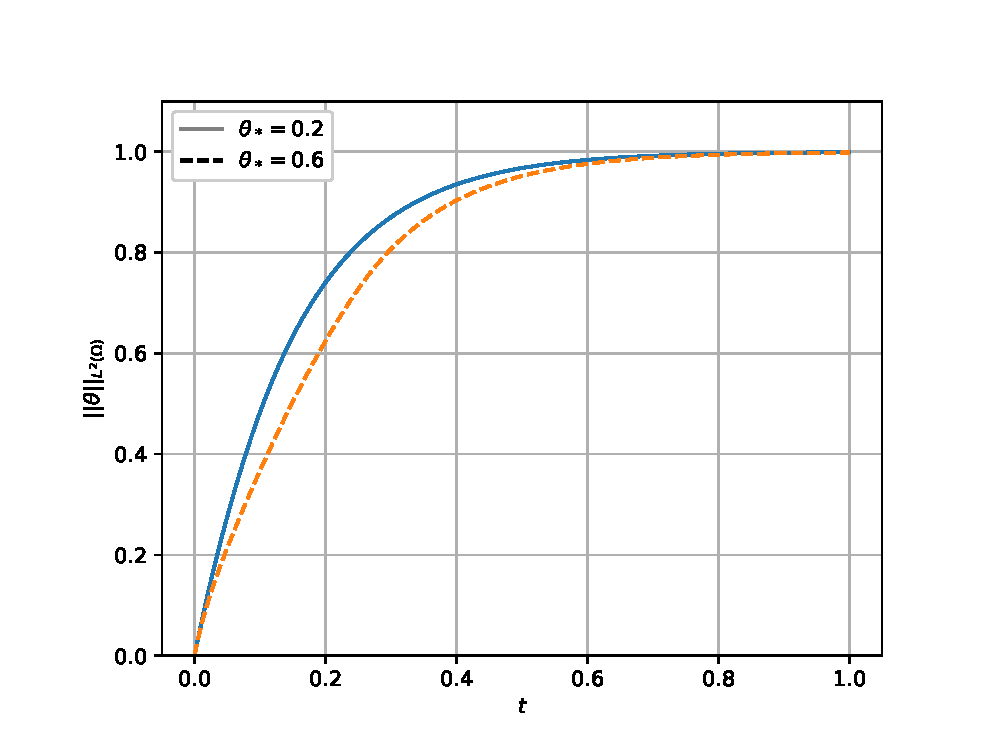
\includegraphics[width=1\linewidth]{additional/3/theta_dyn_star} \\ а) Первый эксперимент
    \end{minipage}
    \hfill
    \begin{minipage}[b][][b]{0.49\linewidth}
        \centering
        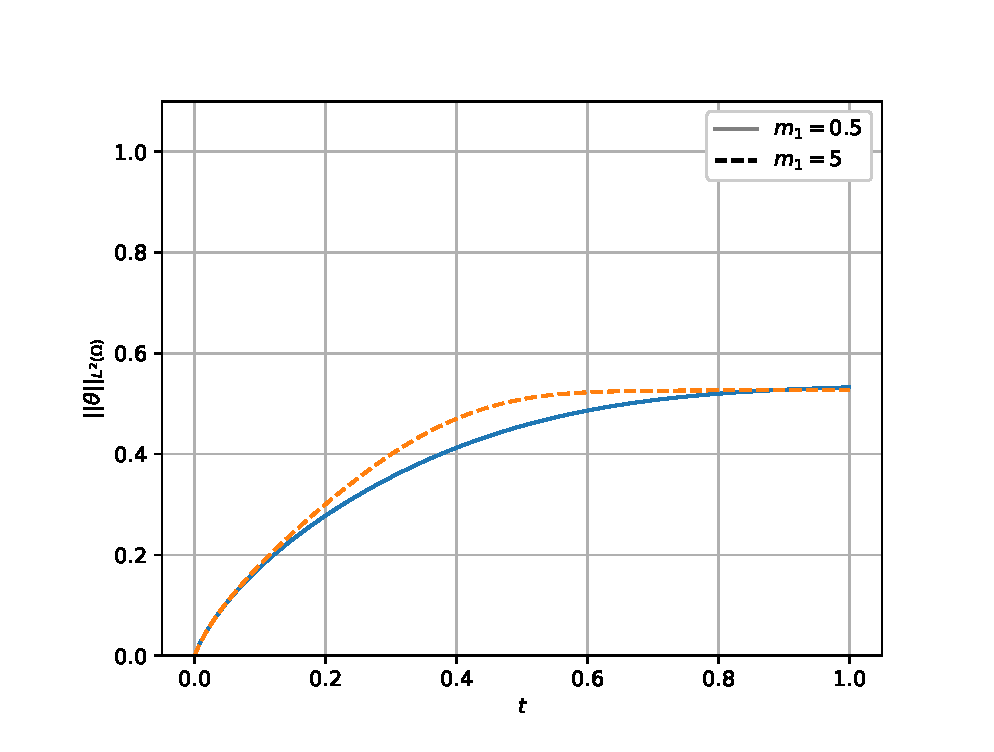
\includegraphics[width=1\linewidth]{additional/3/theta_dyn_m} \\ б) Второй эксперимент
    \end{minipage}
    \caption{$||\theta||_{L(\Omega)}$ при различных $a(\theta)$}
    \label{fig:4_3:theta_dyn_diff}
\end{figure}

Из приведённых примеров видно, что параметр $a(\theta)$ может оказывать существенное влияние
на динамику температурного поля.
Приведём изолинии $\theta(T)$, получившиеся в результате второго эксперимента.
\begin{figure}[h!t]
    \begin{minipage}[b][][b]{0.49\linewidth}
        \centering
        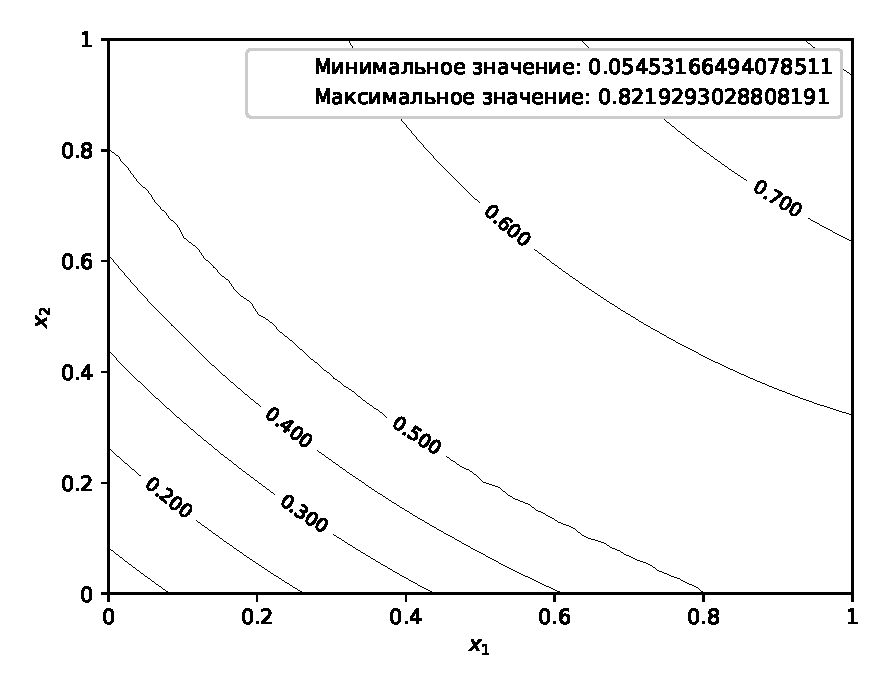
\includegraphics[width=1\linewidth]{additional/3/theta_iso_1} \\ а) $m_1 = 0.5$,
    \end{minipage}
    \hfill
    \begin{minipage}[b][][b]{0.49\linewidth}
        \centering
        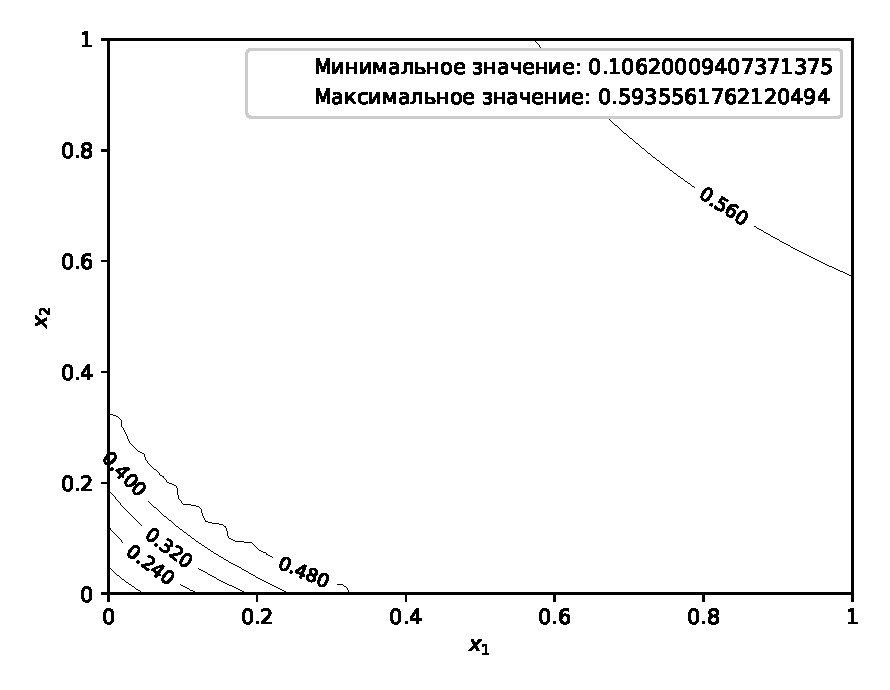
\includegraphics[width=1\linewidth]{additional/3/theta_iso_2} \\ б) $m_1 = 5$.
    \end{minipage}
    \caption{Тепмературное поле $\theta (T)$}
    \label{fig:4_3:theta_iso_2exp}
\end{figure}

В первом эксперименте температурное поле сходится к $1$ при любой функции $a$.
Полученные анимации (которые невозможно привести здесь), а также
соответствующий код экспериментов можно найти по ссылке~\cite{mesenev-github}.



%Перенос тепла и излучения будет рассматриваться в среде,
%состоящей из четырех частей, которые интерпретируются как кровь,
%стенки вены, около-венозная ткань и оптическое волокно.
%Вычислительная область в цилиндрической системе координат в случае
%угловой симметрии схематически изображена на рисунке~\ref{fig:4_3:3}
%(линейные размеры указаны в миллиметрах).
%
%\begin{figure}[h!t]
%    \centerfloat{\includegraphics[scale=0.35]{6_cheb/1}}
%    \caption{Область вычисления}
%    \label{fig:4_3:3}
%\end{figure}
%%\ref{fig:4_3:3}
%Для нахождения решения начально-краевой
%задачи~\eqref{eq:1_6:1}--\eqref{eq:1_6:3}
%мы дискретизируем временной интервал
%$(0, T), \quad 0=t_{0}<t_{1}<t_{2}<\ldots<t_{N}=T$.
%Для каждого момента времени $t=t_{l}=l \Delta t, l=1,2, \ldots, N$,
%используется итерационный алгоритм для нахождения решения соответствующей
%краевой задачи. $n$-й шаг итерационной процедуры $(n=1,2, \ldots, M)$
%записывается следующим образом:
%\begin{gather}
%    -\operatorname{div}\left(\alpha \nabla \varphi_{n}\right)
%    +\beta\left(\varphi_{n}-\theta_{n-1}^{3}
%    \left|\theta_{n-1}\right|\right)=g, \label{eq:3_1:22}\\
%    \sigma \partial \theta_{n} / \partial t
%    -\operatorname{div}\left(k\left(\theta_{n-1}\right)
%    \nabla \theta_{n}\right)
%    -b\left(\theta_{n-1}^{3}\left|\theta_{n}\right|
%    -\varphi_{n}\right)=f, \quad x \in \Omega, \label{eq:3_1:23}\\
%    k\left(\theta_{n-1}\right) \partial_{n} \theta_{n}
%    +\left.p\left(\theta_{n}-\theta_{b}\right)\right|_{\Gamma}=0,
%    \quad \alpha \partial_{n} \varphi_{n}+\left.\gamma
%    \left(\varphi_{n}-\theta_{b}^{4}\right)\right|_{\Gamma}=0,\label{eq:3_1:24}
%\end{gather}
%где производная по времени в~\eqref{eq:3_1:23}
%аппроксимируется как:
%\[
%    \frac{\partial \theta_{n}}{\partial t} \simeq
%    \frac{
%        \left.\theta_{n}\right|_{t=t_{l}}
%        -\left.\theta_{M}\right|_{t=t_{l-1}}
%    }{\Delta t},
%\]
%и функции $\theta_{n}, \theta_{n-1}, \varphi_{n}$
%в~\eqref{eq:3_1:22}--\eqref{eq:3_1:24} являются приближениями решения,
%соответствующими моменту времени $t=t_{l}$.
%Подстрочный индекс функций
%$\theta_{n}, \theta_{n-1}$ и $\varphi_{n}$ означает номер итерации.
%Для инициализации итерационной процедуры задаем начальное приближение
%температуры для каждого момента времени:
%\begin{equation}
%    \label{eq:3_1:25}
%    \left.\theta_{0}\right|_{t=t_{l}}=
%    \left.\theta_{M}\right|_{t=t_{l-1}},
%    \quad l=1,2, \ldots, N, \left.\quad
%    \theta_{M}\right|_{t=t_{0}}=\theta_{i n}.
%\end{equation}
%
%В уравнениях~\eqref{eq:3_1:22},~\eqref{eq:3_1:23}
%$g=P_{\varphi} \chi / \mathcal{M}_{\varphi},
%f=P{\theta} \chi / \mathcal{M}_{\theta}$,
%где $P{\varphi}$ --  мощность источника, расходуемая на излучение,
%$P_{\theta}$ описывает мощность источника, расходуемую на нагрев
%кончика волокна, $\chi$ -- характеристическая функция части среды,
%в которой расположен кончик волокна, деленная на объем кончика волокна,
%$\mathcal{M}_{\varphi}$ и $\mathcal{M}_{\theta}$ --  нормализующие коэффициенты
%для получения средней интенсивности излучения
%и абсолютной температуры из $\varphi$ и $\theta$.
%
%Для реализации каждого шага итерационного
%алгоритма~\eqref{eq:3_1:22}--\eqref{eq:3_1:25}
%использовался метод конечных элементов с использованием
%программного пакета FreeFEM++\cite{Hecht2012}.
%Оптические и термофизические параметры среды
%взяты из~\cite{van2014optical}.
%Параметры $\theta_{b}$ и $\theta_{i n}$ соответствуют
%температуре $37^{\circ} \text{C}$, а коэффициент $\gamma$ равен 1.
%Во всех расчетах начальное положение кончика оптического волокна
%соответствует $(r, z)=(0,5)$, и его скорость отката составляет
%$2 \text{~мм} / \text{с}$.
%Следуя~\cite{van2014optical, Some_Poluektova2014},
%мы моделируем теплоперенос потоком пузырьков,
%образующихся на горячем кончике волокна, через коэффициент теплопроводности,
%зависящий от температуры, как следующим образом: когда температура
%в определенной точке достигает $95^{\circ}\text{~C}$ и выше,
%коэффициент теплопроводности увеличивается в 200 раз.
%
%Эффективность лазерной абляции можно оценить по поведению
%температурных профилей в различных точках вычислительной области.
%Основные параметры процедуры лазерной абляции -- мощность лазера,
%длина волны излучения, скорость отката оптического волокна и
%соотношение между мощностями лазера, затрачиваемыми на
%излучение и нагрев кончика волокна.
%
%Отметим, что решение задачи~\eqref{eq:1_6:1}--\eqref{eq:1_6:3} зависит от длины
%волны неявным образом, через параметры $\alpha$ и $\beta$,
%описывающие свойства излучения среды (смотрите таблицы значений коэффициента
%поглощения и коэффициента уменьшения рассеяния, определяющие параметры
%$\alpha$ и $\beta$~\cite{van2014optical, Some_Poluektova2014}).
%Как правило, лазерная абляция осуществляется излучением с длиной волны
%от \(810\) до $1950$~нм.
%Достаточно широко используемые диапазоны скорости отката волокна и мощности
%лазерного излучения составляют $1-3\text{~мм}/\text{с}$
%и $5-15$~Вт
%соответственно~\cite{
%    Mathematical_Mordon2006,
%    van2014optical,
%    Some_Poluektova2014}.
%
%
%\begin{figure}[h!t]
%    \centerfloat{\includegraphics[scale=0.33]{6_cheb/2}}
%    \caption{Поведение температуры в точке $(1.5,10)$
%        при мощности лазера $10\text{~Вт}$ и следующих длинах волн:
%        $810\text{~нм}$ (черный), $1064\text{~нм}$ (красный),
%        $1470\text{~нм}$ (зеленый) и $1950\text{~нм}$ (синий).}
%    \label{fig:4_3:4}
%\end{figure}
%
%Рисунок~\ref{fig:4_3:4} показывает поведение температурных профилей в точке $(1.5,10)$ для
%излучения с различными длинами волн: $810 \text{~нм}, 1064 \text{~нм},
%1470 \text{~нм}$ и $1950 \text{~нм}$.
%Мощность источника устанавливается как $\left(P_{\varphi}, P_{\theta}\right)
%=(7 \text{~Вт}, 3 \text{~Вт})$ во всех случаях.
%Как видно из рисунка~\ref{fig:4_3:4}, изменение длины волны излучения оказывает
%значительное влияние на поведение температурного профиля.
%Тем не менее, возможно обеспечить достаточно близкую продолжительность
%кипения (когда температура выше $95^{\circ} \text{C}$) для температурных
%профилей, соответствующих разным длинам волн, изменив мощность
%лазера $P=P_{\varphi}+P_{\theta}$, сохраняя соотношение
%$P_{\varphi} / P_{\theta}$ равным $7 / 3$ (рисунок~\ref{fig:4_3:4}).
%Отметим, что рассчитанная температура в точках перивенозной ткани,
%$(2.5,10)$ и $(3.5,10)$, довольно безопасна (рисунок~\ref{fig:4_3:5}).
%
%Как видно из проведенных экспериментов, использование компьютерного
%моделирования является перспективным способом определения оптимальных
%параметров излучения, обеспечивающих эффективную и безопасную процедуру ВВЛА.
%
%На рисунке~\ref{fig:4_3:4} показаны температурные профили
%в точке $(1.5, 10)$ для мощности лазера
%$10 \text{~Вт}$ и для разных длин волн: $810 \text{~нм}$ (черный),
%$1064 \text{~нм}$ (красный), $1470 \text{~нм}$
%(зеленый) и $1950 \text{~нм}$ (синий).
%
%\begin{figure}[h!t]
%    \centerfloat{\includegraphics[scale=0.33]{6_cheb/3}}
%    \caption{Поведение температуры в точке $(1.5,10)$
%        для следующих длин волн и мощностей лазера:
%        $810 \text{~нм}, P=10 \text{~Вт}$ (черный);
%        $1064 \text{~нм}, P=11 \text{~W}$ (красный);
%        $1470 \text{~нм}, P=7,5 \text{~W}$ (зеленый);
%        $1950 \text{~нм}, P=6 \text{~W}$ (синий).}
%    \label{fig:4_3:5}
%\end{figure}
%На рисунке~\ref{fig:4_3:5} показаны температурные профили в точке $(1.5,10)$ для разных
%длин волн и мощности лазера: $810 \text{~нм}$, $P=10 \text{~Вт}$
%(черный); $1064 \text{~нм}, P=11 \text{~Вт}$ (красный);
%$1470 \text{~нм}, P=7.5 \text{~Вт}$ (зеленый);
%$1950 \text{~нм}, P=6 \text{~Вт}$ (синий).
%
%
%\begin{figure}[h!t]
%    \centerfloat{\includegraphics[scale=0.33]{6_cheb/4}}
%    \caption{Поведение температуры в точках $(1.5,10)$ (сплошная линия),
%        $(2.5,10)$ (пунктирной линией) и $(3,5,10)$ (пунктирной линией с точкой).
%        Длина волны равна $810 \text{~нм},\left(P_{\varphi},
%        P_{\theta}\right)=(7 \text{~W}, 3 \text{~W})$.}
%    \label{fig:4_3:6}
%\end{figure}
%На рисунке~\ref{fig:4_3:6} показаны температурные профили в точках $(1.5,10)$ (сплошной),
%$(2.5,10)$ (пунктирный) и $(3.5,10)$ (точка-тире).
%Длина волны составляет $810 \text{~нм},\left(P_{\varphi},
%P_{\theta}\right)=(7 \text{~Вт}, 3 \text{~Вт})$
%
%
%%Chebotarev_2 nd, Chebotarev_Park_Mesenev_Kovtanyuk_21
%
%\subsection{Метод штрафов для задачи с фазовыми ограничениями}
%\label{subsec:ch4/sec3/subsec5}
%Квазилинейная модель радиационного и диффузионного теплообмена в ограниченной области
%$\Omega \subset \mathbb{R}^{3}$ с границей $\Gamma=\partial \Omega$
%в разделе~\ref{sec:ch3:sec2} представлена в виде начально-краевой задачи
%следующим образом:
%\begin{equation*}
%    \begin{aligned}
%        & \sigma \partial \theta / \partial t-\operatorname{div}(k(\theta) \nabla \theta)-\beta \varphi=u_{1} \chi, \\
%        & -\operatorname{div}(\alpha \nabla \varphi)+\beta \varphi=u_{2} \chi, \quad x \in \Omega, \quad t \in(0, T), \\
%        & \theta=\left.0\right|_{\Gamma}, \quad \alpha \partial_{n}
%        \varphi+\left.2^{-1} \varphi\right|_{\Gamma}=0,\left.\quad \theta\right|_{t=0}=\theta_{0}.
%    \end{aligned}
%\end{equation*}
%Требуется найти неизвестные интенсивности $u_1,\, u_2$ и соответствующие поля $\theta, \, \varphi$
%по условию
%\[
%    J(\theta)=\int_{0}^{T}
%    \int_{G_{1}}\left(\theta-\theta_{d}\right)^{2} d x d t \rightarrow \inf,
%\]
%при ограничениях
%\[
%    u_{1,2} \geq 0, \quad u_{1}+u_{2} \leq P,\left.\quad \theta\right|_{G_{2}} \leq \theta_{*}.
%\]
%
%В разделе~\ref{subsec:ch3/sec2/penalty} показано, что задачу с ограничениями
%на температуру в области $G_2$ можно
%аппроксимировать задачей со штрафом $P_\varepsilon$.
%
%
%Рассмотрим итерационный алгоритм решения задачи оптимального управления
%$P_{\varepsilon}$ для случая, когда параметры управления
%$u_{1}$ и $u_{2}$ не зависят от времени.
%На каждой итерации алгоритма
%решается линейно-квадратичная задача оптимального управления,
%в которой требуется найти минимум функционала
%\begin{equation}
%    \label{eq:3_2:9}
%    \widehat{J}_{\varepsilon}(\theta)=\int_{0}^{T}
%    \int_{G_{1}}\left(\theta-\theta_{d}\right)^{2} dx dt
%    +\frac{1}{\varepsilon} \int_{0}^{T}
%    \int_{G_{*}}\left(\theta-\theta_{*}\right)^{2} dx dt
%    \rightarrow \inf, \quad u\in U_{ad}
%\end{equation}
%с соответствующими ограничениями
%\begin{equation}
%    \label{eq:3_2:10}
%    \begin{gathered}
%        \sigma \partial \theta / \partial t-\operatorname{div}(k(\widehat{\theta})
%        \nabla \theta)=u, \quad x \in \Omega, \quad 0<t<T, \\
%        \left.\theta\right|_{\Gamma}=0, \quad \theta(x, 0)=\theta_{0}.
%    \end{gathered}
%\end{equation}
%Здесь
%\[
%    \begin{gathered}
%        U_{a d}=\left\{u=u_{1} \chi+u_{2} \beta B^{-1} \chi: u_{1,2} \in \mathbb{R},\right.
%        \left.u_{1,2} \geq 0, u_{1}+u_{2} \leq P\right\}, \\
%        G_{*}=\left\{x \in G_{2}: \hat{\theta}(x, t)>\theta_{*}\right\}.
%    \end{gathered}
%\]
%
%Функция $\widehat{\theta}$ описывает поле температуры,
%найденное на предыдущей итерации.
%В качестве зависимости коэффициента теплопроводности от температуры используется
%гладкая аппроксимация кусочно-постоянной функции, рассмотренная
%в~\cite{van2014optical, Some_Poluektova2014, Endovenous_Malskat2014}.
%
%Как легко видеть, задача~\eqref{eq:3_2:9},~\eqref{eq:3_2:10} сводится к
%нахождению минимума квадратичной функции параметров $u_{1}$ и $u_{2}$
%\[
%    \widehat{J}_{\varepsilon}\left(u_{1} \theta_{1}+u_{2} \theta_{2}+\theta_{3}\right) \rightarrow \inf
%\]
%на треугольнике $\left\{u_{1}, u_{2} \in \mathbb{R}:
%u_{1,2} \geq 0, u_{1}+u_{2} \leq P\right\}$.
%Функции $\theta_{1}, \theta_{2}$ и $\theta_{3}$
%вычисляются заранее как решения следующих линейных
%начально-краевых задач для $x \in \Omega, t \in(0, T)$:
%\[
%    \begin{aligned}
%        &\sigma \partial \theta_{1} / \partial t-\operatorname{div}\left(k(\widehat{\theta})
%        \nabla \theta_{1}\right)=\chi, &
%        \left.\theta_{1}\right|_{\Gamma}=0, \quad \theta_{1}(x, 0)=0, \\
%        &\sigma \partial \theta_{2} / \partial t-\operatorname{div}\left(k(\widehat{\theta})
%        \nabla \theta_{2}\right)=\beta B^{-1} \chi, &
%        \left.\theta_{2}\right|_{\Gamma}=0, \quad \theta_{2}(x, 0)=0, \\
%        &\sigma \partial \theta_{3} / \partial t-\operatorname{div}\left(k(\widehat{\theta})
%        \nabla \theta_{3}\right)=0, &
%        \left.\theta_{3}\right|_{\Gamma}=0, \quad \theta_{3}(x, 0)=\theta_{0}.
%    \end{aligned}
%\]
%
%При проведении численных экспериментов использовалась область,
%аналогичная рассматриваемой в разделе~\ref{subsec:ch4/sec3/quasilinear}
%(рисунок~\ref{fig:4_3:3}).
%Толщина карбонизированного слоя равна $0,2 \text{~мм}$,
%скорость вытягивания волокна $2 \text{~мм}/\text{с}$.
%Рассматривалось излучение с длиной волны $1064 \text{~нм}$.
%Оптические и теплофизические параметры среды взяты
%из~\cite{van2014optical, Some_Poluektova2014, Endovenous_Malskat2014}.
%
%
%Для демонстрации сходимости итерационного алгоритма в качестве
%решения прямой начально-краевой задачи для $\left(u_{1}, u_{2}\right)=( 3,7)$
%(здесь и далее единицы в ваттах).
%Области $G_{1}$ и $G_{2}$ берутся как достаточно малые окрестности
%точек $(1.5,10),(3.5,10)$.
%Для реализации итерационного алгоритма мы взяли $\varepsilon=0.3$ и $\theta_{*}$,
%соответствующие $47^{\circ} \text{C}$.
%
%
%\begin{figure}[h!t]
%    \centerfloat{\includegraphics[scale=0.33]{2_cheb/2}}
%    \caption{Температурные профили: желаемая температура (черный),
%        1-е (зеленое), 2-е (синее) и 3-е (красное) приближения.}
%    \label{fig:4_3:7}
%\end{figure}
%
%
%
%Аппроксимации решения в точке $(1.5,10)$ показаны на рисунке~\ref{fig:4_3:7}.
%Аппроксимации после первого, второго и третьего шагов итерационного
%алгоритма отмечены зеленым цветом
%$\left(u_{1 }, u_{2}\right)=(2.5,4.8)$,
%синим  $\left(u_{1}, u_{2}\right)=(3.4,3.5)$
%и красным $\left(u_{1}, u_{2}\right)=(4.2,0.9)$ соответственно.
%Черная линия показывает желаемую температуру, соответствующую
%$\left(u_{1}, u_{2}\right)=(3,7)$.
%Максимальное значение температуры в точке $(3.5,10)$ равно $48,8^{\circ}\text{C}$.
%Отметим, что при $\left(u_{1}, u_{2}\right)=(3,7)$ максимальное значение
%температуры в точке $(3.5,10)$ равно $50,2^{ \circ} \text{C}$.
%
%Данный пример демонстрирует возможность снижения температуры в
%околовенозной ткани при сохранении температурного режима внутри вены.

    \section{Алгоритмы решения задач с данными Коши. Примеры.}\label{sec:ch4/sec4}

%VYC0036
\subsection{
    Решение задачи сложного теплообмена
с граничными условиями типа коши
}\label{subsec:ch4/sec4/subsec1}

%jvm-mesenev-chebotarev
\subsection{
    Задача сложного теплообмена с условиями
    Коши для температуры на части границы
}\label{subsec:ch4/sec4/subsec2}


    \chapter*{Заключение}                       % Заголовок
\addcontentsline{toc}{chapter}{Заключение}  % Добавляем его в оглавление

%% Согласно ГОСТ Р 7.0.11-2011:
%% 5.3.3 В заключении диссертации излагают итоги выполненного исследования, рекомендации, перспективы дальнейшей разработки темы.
%% 9.2.3 В заключении автореферата диссертации излагают итоги данного исследования, рекомендации и перспективы дальнейшей разработки темы.
%% Поэтому имеет смысл сделать эту часть общей и загрузить из одного файла в автореферат и в диссертацию:

%% Согласно ГОСТ Р 7.0.11-2011:
%% 5.3.3 В заключении диссертации излагают итоги выполненного исследования, рекомендации, перспективы дальнейшей разработки темы.
%% 9.2.3 В заключении автореферата диссертации излагают итоги данного исследования, рекомендации и перспективы дальнейшей разработки темы.
В диссертации доказано существование квазирешения задачи нахождения
коэффициента отражения участка границы для стационарной модели,
по дополнительной информации о температурном поле.
Экспериментально поверена устойчивость получаемых
решений методом градиентного спуска.
Таким образом, получены важные с теоретической точки зрения результаты,
которые могут быть полезны при дальнейшем использовании
стационарных моделей сложного теплообмена и анализе обратных
задач в рамках нестационарных моделей сложного теплообмена.
Развитые методы исследования начально-краевых задач могут
применяться для изучения различных моделей, описываемых нелинейными
уравнениями со сходной структурой.

Разработанный комплекс программ для постановки численных экспериментов
показал свою надёжность и может в дальнейшем быть использован как
пример для решения подобных задач.

Разработан комплекс программ для проведения вычислительных экспериментов.
Для презентации результатов расчётов, помимо самих солверов,
был разработан программный комплекс для отрисовки
полученных расчётов в трёхмерных областях.

Исследование нестационарных моделей сложного теплообмена и соответствующих им
обратных задач является крайне перспективной областью математического моделирования
и в то же время достаточно сложной для теоретического
анализа и реализации численных решений.
Более широкий класс процессов может быть покрыт задачами на оптимальное
управление многими переменными среды, что позволяет более точно находить
решения для инженерных задач.



В заключение автор выражает искреннюю благодарность научному руководителю
А.\ Ю.\ Чеботареву за его поддержку,
помощь, терпеливость и личный пример,
который сделал данную работу возможной.

Особую признательность автор хочет выразить А.\ В.\ Байдину,
Р.\ В.\ Бризицкому, И.\ Л.\ Артемьевой, чья поддержка оказалась
неоценимой в написании данной работы.
А.\ С.\ Кленину, который стал источником мотивации в написании данного труда,
и Г.\ В.\ Алексееву за помощь в первых шагах научной деятельности автора.

Автор хотел бы отдельно поблагодарить В.\ П.\ Месенева
за его вклад в становление автора
и бесконечную сопричастность к данной работе.
      % Заключение
%    \input{Dissertation/acronyms}        % Список сокращений и условных обозначений
%    \input{Dissertation/dictionary}      % Словарь терминов
    \input{Dissertation/references}      % Список литературы
    \input{Dissertation/lists}           % Списки таблиц и изображений (иллюстративный материал)

    \setcounter{totalchapter}{\value{chapter}} % Подсчёт количества глав

%%% Настройки для приложений
    \appendix
% Оформление заголовков приложений ближе к ГОСТ:
    \setlength{\midchapskip}{20pt}
    \renewcommand*{\afterchapternum}{\par\nobreak\vskip \midchapskip}
    \renewcommand\thechapter{\Asbuk{chapter}} % Чтобы приложения русскими буквами нумеровались

    \chapter{Приложения}
\label{ch:ch5}
        % Приложения

    \setcounter{totalappendix}{\value{chapter}} % Подсчёт количества приложений

\end{document}
